\documentclass[aspectratio=169,10pt]{beamer}
\usetheme{metropolis}
\usepackage{amsmath,amssymb,bm}
\usepackage{siunitx}
\usepackage{booktabs}
\usepackage[table]{xcolor}
\usepackage{tikz}
\usetikzlibrary{arrows.meta,calc,positioning,patterns}
\usepackage{pgfplots}
\pgfplotsset{compat=1.17}
\sisetup{per-mode=symbol,detect-all}
\metroset{numbering=fraction,progressbar=frametitle,block=fill}
\tikzset{capt/.style={text width=5.2cm,align=center}}
\hypersetup{colorlinks=true,urlcolor=blue!60!black,linkcolor=.}
\addtobeamertemplate{frametitle}{}{%
  \begin{tikzpicture}[remember picture,overlay]
    \node[anchor=north east,yshift=-1.5pt,xshift=-6pt] at (current page.north east) {
\includegraphics[height=0.7cm]{logos/itu_logo_beyaz.pdf}};
  \end{tikzpicture}}
\titlegraphic{\hfill
\includegraphics[height=1.6cm]{logos/itu_logo_laci.pdf}}

\title{Lecture 5: Thread Standards and Power Screws}
\subtitle{UCK 364E Design of Machine Elements}
\author{Prof.\ Dr.\ Onur Tunçer}
\institute{Department of Aeronautical Engineering, Istanbul Technical University}
\date{Fall 2026}

\begin{document}
\maketitle

\begin{frame}{Today}
\begin{enumerate}
  \item Two jobs for a helix --- and the oldest screw of all
  \item Thread geometry: pitch, lead, the three diameters, the helix angle
  \item The two standards systems, and how to read a designation
  \item The aerospace profiles: UNJ and MJ, and why they exist
  \item Tensile stress area
  \item Cut versus rolled --- and \emph{rolled after heat treatment}
  \item Heads, drives and countersinks --- and the knife edge
  \item Nuts, locking, and the preload you actually get
  \item Materials and environment --- galling, galvanic, temperature, composites
  \item Power screws: torque, self-locking, efficiency
  \item Thread bearing pressure, and why wear sets the life
  \item The stabiliser trim jackscrew
\end{enumerate}
\end{frame}

\begin{frame}{A helix does two different jobs}
\begin{columns}[T]
\begin{column}{0.47\textwidth}
\metroset{block=fill}
\begin{block}{Fastening}
Convert torque into a large \emph{clamping force}.\\[4pt]
An airliner has of the order of \textbf{a million} of them.\\[4pt]
You want high efficiency at making preload, a benign root in fatigue --- and
\textbf{no motion at all}.
\end{block}
\end{column}
\begin{column}{0.47\textwidth}
\begin{block}{Motion}
Convert rotation into \emph{translation}.\\[4pt]
Flaps, slats, landing gear, cargo doors, stabiliser trim.\\[4pt]
You want it to move under load --- and in most aircraft uses, to \textbf{stop and hold}
the moment the drive is removed.
\end{block}
\end{column}
\end{columns}
\vfill
\begin{alertblock}{The tension that organises this lecture}
A thread that slides easily is efficient but will not hold. A thread that holds wastes most of the
power you put in. There is no thread form that escapes this.
\end{alertblock}
\end{frame}

\begin{frame}{The oldest screw is a pump}
\centering
\resizebox{!}{4.9cm}{% The Archimedes screw: the same helix, carrying material instead of clamping.
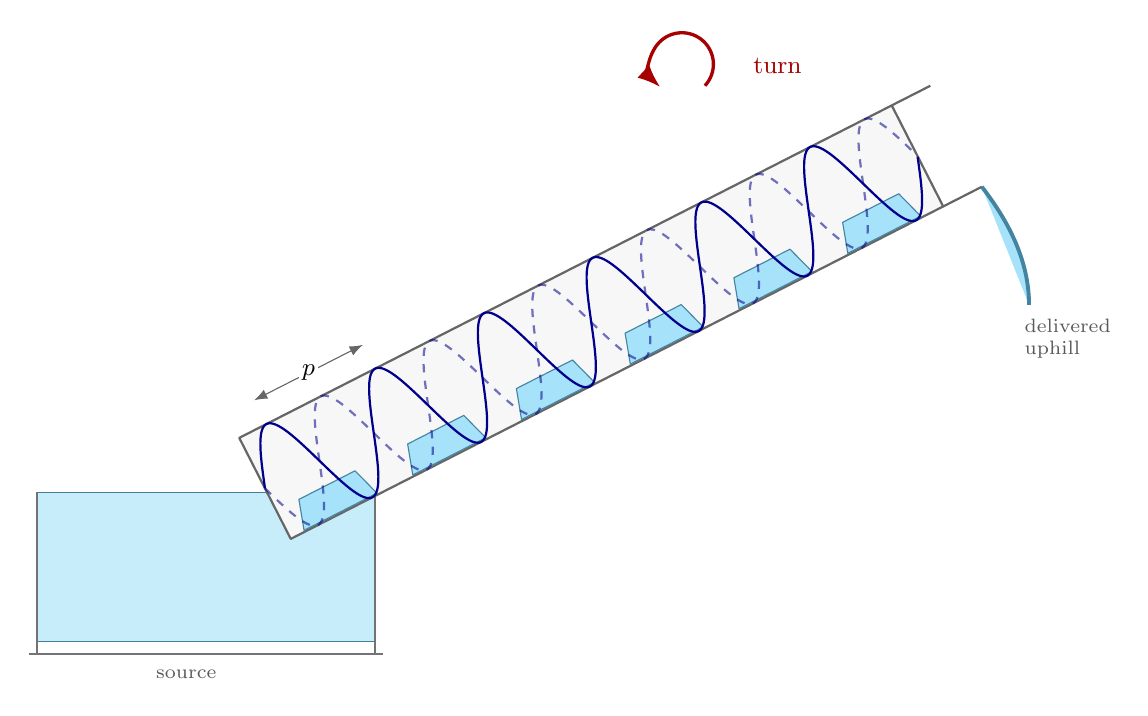
\begin{tikzpicture}[>=Latex,line join=round]
\tikzset{
  water/.style={fill=cyan!35,draw=cyan!60!black,thin},
  tube/.style={draw=black!60,thick},
  flight/.style={draw=blue!55!black,thick},
  lb/.style={font=\small},
  sm/.style={font=\scriptsize,text=black!65}
}
\def\ang{27}      % inclination
\def\r{0.72}      % tube radius
\def\p{1.55}      % pitch (projected)
\def\Lx{9.3}      % length along the axis

% ---------- lower reservoir ----------
\fill[cyan!22,draw=cyan!55!black] (-2.90,-1.95) rectangle (1.40,-0.05);
\draw[black!55,thick] (-2.90,-2.10) -- (-2.90,-0.05) (1.40,-2.10) -- (1.40,-0.05);
\draw[black!55,thick] (-3.00,-2.10) -- (1.50,-2.10);
\node[sm,anchor=north] at (-1.0,-2.18) {source};

\begin{scope}[rotate=\ang]

% ---------- tube ----------
\draw[tube,fill=black!3] (0,-\r) rectangle (\Lx,\r);

% ---------- water pockets, one per pitch, lying on the low side ----------
\foreach \i in {0,1,...,5}{
  \pgfmathsetmacro\xc{0.72+\i*\p}
  \fill[water] (\xc-0.52,-\r+0.02) -- (\xc+0.52,-\r+0.02)
     -- (\xc+0.40,-\r+0.40) -- (\xc-0.40,-\r+0.40) -- cycle;
}

% ---------- the flight: near edge solid, far edge dashed ----------
\draw[flight,domain=0:\Lx,samples=400,variable=\x]
  plot ({\x},{\r*sin(360*\x/\p)});
\draw[flight,dashed,opacity=0.55,domain=0:\Lx,samples=400,variable=\x]
  plot ({\x},{-\r*sin(360*\x/\p)});

% ---------- pitch dimension ----------
\draw[<->,gray!80!black,thin] (0.385,\r+0.34) -- (0.385+\p,\r+0.34);
\node[font=\small,fill=white,inner sep=1pt] at (0.385+\p/2,\r+0.34) {$p$};

% ---------- rotation ----------
\draw[->,red!65!black,very thick] ({\Lx-2.0},{\r+1.30}) arc (-70:200:0.40);
\node[font=\small,text=red!65!black,anchor=west] at ({\Lx-1.45},{\r+1.30}) {turn};

% ---------- outlet ----------
\draw[tube] (\Lx,\r) -- (\Lx+0.55,\r) (\Lx,-\r) -- (\Lx+0.55,-\r);
\end{scope}

% ---------- discharge ----------
\coordinate (out) at ({(\Lx+0.55)*cos(\ang)-(-\r)*sin(\ang)},{(\Lx+0.55)*sin(\ang)+(-\r)*cos(\ang)});
\draw[water,line width=1.4pt,draw=cyan!60!black] (out) .. controls +(0.35,-0.45) and +(0,0.55) .. ($(out)+(0.6,-1.5)$);
\node[sm,anchor=north west,align=left] at ($(out)+(0.42,-1.55)$) {delivered\\ uphill};

\end{tikzpicture}
}
\vfill
\raggedright
\textbf{The same helix, the other job.} The flight is open, so the \emph{water} --- not a nut ---
is what travels along the axis. Hold a nut on it instead and the nut travels: a power screw. Make
the lead so small it cannot back-drive, and it is a bolt.
\end{frame}

\begin{frame}{One geometry, three machines}
\centering\small
\begin{tabular}{@{}lll@{}}
\toprule
Hold still & Turn & What you get\\
\midrule
the nut & the screw & a \textbf{power screw} --- the nut translates\\
nothing: an open flight & the screw & an \textbf{Archimedes screw} --- the \emph{material} translates\\
the nut, tiny lead & the screw & a \textbf{bolt} --- too slow to back-drive\\
\bottomrule
\end{tabular}
\vfill
\raggedright
\begin{block}{The relations do not care which one you built}
$L=np$ \quad and \quad $\tan\lambda = L/\pi d_m$ \quad hold for all three. Only the \textbf{useful
output} differs: axial transport, axial force, or a clamping force that must never move.
\end{block}
\vfill
{\footnotesize Vitruvius specifies \textbf{eight} starts --- a multi-start thread, chosen for lead
per turn, exactly as you would choose one today.}
\end{frame}

\begin{frame}{Archimedes of Syracuse, 287--212 BC}
The earliest references to the water screw date from \textbf{250--220 BC}.
\vfill
\begin{columns}[T]
\begin{column}{0.56\textwidth}
{\footnotesize
\textbf{Moschion}, on the ship \emph{Syracusia} --- her bilge could be emptied by \alert{one man}
using ``an invention of Archimedes''. The first screw to go to sea went as a pump.
\vspace{3pt}

\textbf{Diodorus Siculus} (1st c.\ BC) --- irrigating the Nile delta, and draining the Roman silver
mines in Spain, where he calls it the ``Egyptian screw''.
\vspace{3pt}

\textbf{Vitruvius}, \emph{De architectura} X.6 (27--22 BC) --- the earliest surviving
\emph{construction} account: how to set out the spiral, how many starts, at what inclination.}
\end{column}
\begin{column}{0.40\textwidth}
\begin{alertblock}{\normalsize But is it his?}
{\footnotesize Stephanie Dalley reads an inscription of \textbf{Sennacherib} as describing bronze
water screws irrigating the gardens at Nineveh --- centuries earlier. J.\,P.\ Oleson notes that no
ancient source ever explains \emph{why} the device carries Archimedes' name.
\vspace{3pt}

Engineering history is like this more often than textbooks admit.}
\end{alertblock}
\end{column}
\end{columns}
\vfill
{\footnotesize It still works: sewage plants (indifferent to solids and to varying flow), the Dutch
polders --- and since the 1990s, run \alert{backwards} as low-head hydro turbines,
\SIrange{0.01}{14.5}{m^3/s} over heads of \SIrange{0.1}{10}{m}. A screw driven backwards by its load
is a screw that is \textbf{not self-locking} --- which is exactly what a stabiliser jackscrew must
never be.}
\end{frame}

\section{Thread geometry}

\begin{frame}{Pitch, lead and starts}
\begin{columns}[T]
\begin{column}{0.56\textwidth}
\textbf{Pitch} $p$ --- axial distance between adjacent threads.\\[6pt]
\textbf{Lead} $L$ --- axial advance per \emph{turn}.\\[6pt]
\[\boxed{L = n\,p}\qquad n = \text{number of starts}\]
\vspace{4pt}
Multiple starts buy speed and cost self-locking.\\[4pt]
Common in cheap mechanisms.\\
\textbf{Rare in flight-critical ones.}
\end{column}
\begin{column}{0.40\textwidth}
\begin{block}{The three diameters}
\small
$d$ \ major --- at the crests, the nominal size\\[3pt]
$d_3$ \ minor --- at the roots, \emph{where it breaks}\\[3pt]
$d_2$ \ pitch --- thread and groove equally wide; \emph{this is what controls fit}
\end{block}
\end{column}
\end{columns}
\end{frame}

\begin{frame}{Pitch is not lead --- and the difference costs you self-locking}
\centering
\resizebox{!}{4.6cm}{
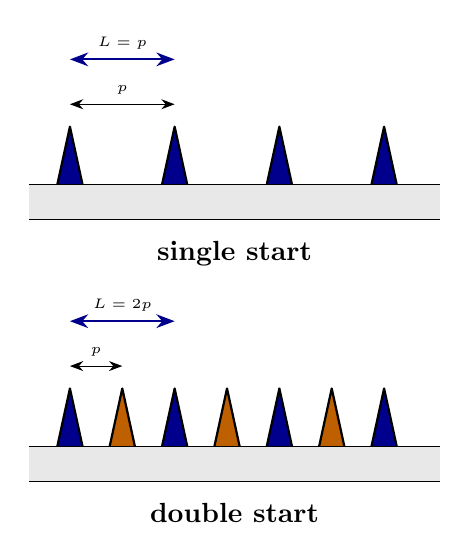
\begin{tikzpicture}[scale=0.95,>=Stealth,font=\scriptsize,line join=round]
\def\hh{0.78}
% ---------------- single start ----------------
\begin{scope}
\foreach \x in {0,1.4,2.8,4.2}{
  \fill[blue!55!black] (\x-0.17,0) -- (\x,\hh) -- (\x+0.17,0) -- cycle;
  \draw[thick] (\x-0.17,0) -- (\x,\hh) -- (\x+0.17,0);}
\draw[thick] (-0.55,0) -- (4.95,0); \draw[thick] (-0.55,-0.45) -- (4.95,-0.45);
\fill[gray!18] (-0.55,-0.45) rectangle (4.95,0);
\draw[<->] (0,\hh+0.30) -- (1.4,\hh+0.30) node[midway,above,font=\tiny]{$p$};
\draw[<->,blue!55!black,thick] (0,\hh+0.90) -- (1.4,\hh+0.90)
  node[midway,above,font=\tiny,black]{$L=p$};
\node[anchor=north,font=\bfseries] at (2.2,-0.62) {single start};
\end{scope}
% ---------------- double start ----------------
\begin{scope}[yshift=-3.5cm]
\foreach \x in {0,1.4,2.8,4.2}{
  \fill[blue!55!black] (\x-0.17,0) -- (\x,\hh) -- (\x+0.17,0) -- cycle;
  \draw[thick] (\x-0.17,0) -- (\x,\hh) -- (\x+0.17,0);}
\foreach \x in {0.7,2.1,3.5}{
  \fill[orange!75!black] (\x-0.17,0) -- (\x,\hh) -- (\x+0.17,0) -- cycle;
  \draw[thick] (\x-0.17,0) -- (\x,\hh) -- (\x+0.17,0);}
\draw[thick] (-0.55,0) -- (4.95,0); \draw[thick] (-0.55,-0.45) -- (4.95,-0.45);
\fill[gray!18] (-0.55,-0.45) rectangle (4.95,0);
\draw[<->] (0,\hh+0.30) -- (0.7,\hh+0.30) node[midway,above,font=\tiny]{$p$};
\draw[<->,blue!55!black,thick] (0,\hh+0.90) -- (1.4,\hh+0.90)
  node[midway,above,font=\tiny,black]{$L=2p$};
\node[anchor=north,font=\bfseries] at (2.2,-0.62) {double start};
\end{scope}
\end{tikzpicture}
}
\vfill
\raggedright
{\small The \emph{pitch} is a property of the thread form and does not change. The \emph{lead} is how
far the nut travels per turn. Adding a second start doubles $L$ with $p$ untouched --- so
$\tan\lambda = L/\pi d_m$ doubles, and a screw that was comfortably self-locking may stop being so.}
\end{frame}

\begin{frame}{The \SI{60}{\degree} basic profile --- ISO 68-1 and ASME B1.1}
\centering
\resizebox{0.86\textwidth}{!}{
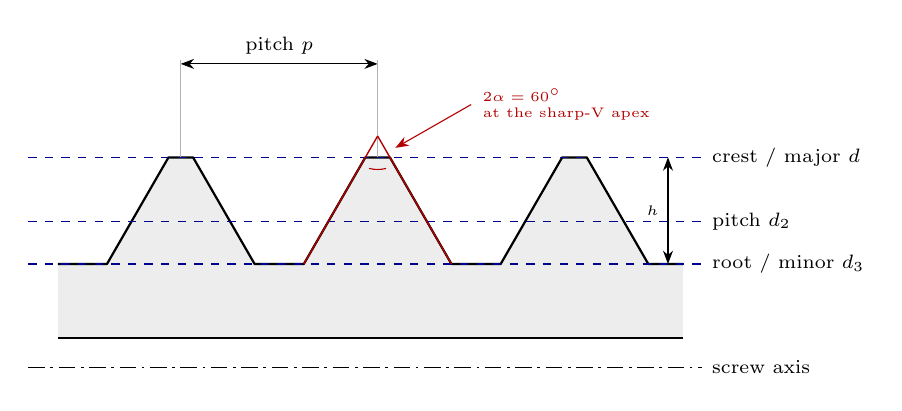
\begin{tikzpicture}[scale=1.25,>=Stealth,font=\scriptsize,line join=round]
\def\hh{1.083}
\fill[gray!14]
  (-0.25,0) -- (0.25,0) -- (0.875,\hh) -- (1.125,\hh) -- (1.75,0) -- (2.25,0)
  -- (2.875,\hh) -- (3.125,\hh) -- (3.75,0) -- (4.25,0) -- (4.875,\hh) -- (5.125,\hh)
  -- (5.75,0) -- (6.1,0) -- (6.1,-0.75) -- (-0.25,-0.75) -- cycle;
\draw[thick]
  (-0.25,0) -- (0.25,0) -- (0.875,\hh) -- (1.125,\hh) -- (1.75,0) -- (2.25,0)
  -- (2.875,\hh) -- (3.125,\hh) -- (3.75,0) -- (4.25,0) -- (4.875,\hh) -- (5.125,\hh)
  -- (5.75,0) -- (6.1,0);
\draw[thick] (-0.25,-0.75) -- (6.1,-0.75);
\draw[blue!55!black,dashed] (-0.55,\hh) -- (6.3,\hh) node[right,black]{crest / major $d$};
\draw[blue!55!black,dashed] (-0.55,0.433) -- (6.3,0.433) node[right,black]{pitch $d_2$};
\draw[blue!55!black,dashed] (-0.55,0) -- (6.3,0) node[right,black]{root / minor $d_3$};
\draw[<->] (1.0,\hh+0.95) -- (3.0,\hh+0.95) node[midway,above]{pitch $p$};
\draw[gray!60,line width=0.3pt] (1.0,\hh) -- (1.0,\hh+0.99);
\draw[gray!60,line width=0.3pt] (3.0,\hh) -- (3.0,\hh+0.99);
% included thread angle: extend the two flanks of one tooth to the sharp-V apex
\draw[red!70!black,line width=0.5pt] (2.25,0) -- (3.0,1.300);
\draw[red!70!black,line width=0.5pt] (3.75,0) -- (3.0,1.300);
\draw[red!70!black] ($(3.0,1.300)+(255.4:0.34)$) arc (255.4:284.6:0.34);
\draw[->,red!70!black,line width=0.4pt] (3.95,1.62) -- (3.18,1.18);
\node[red!70!black,anchor=west,align=left,font=\tiny] at (3.97,1.62)
  {$2\alpha=60^\circ$\\ at the sharp-V apex};
\draw[<->] (5.95,0) -- (5.95,\hh) node[midway,left,font=\tiny]{$h$};
\draw[dash pattern=on 6pt off 2pt on 1pt off 2pt] (-0.55,-1.05) -- (6.3,-1.05);
\node[anchor=west] at (6.3,-1.05) {screw axis};
\end{tikzpicture}
}
\vfill
{\small The flanks carry the load. \alert{The root is the fatigue-critical feature} --- remember this
slide in four minutes.}
\end{frame}

\begin{frame}{Unwrap one turn: the screw is an inclined plane}
\centering
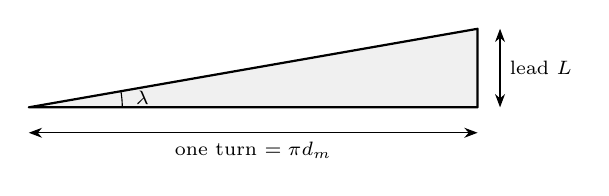
\begin{tikzpicture}[scale=0.95,>=Stealth,font=\scriptsize,line join=round]
\fill[gray!12] (0,0) -- (6.0,0) -- (6.0,1.05) -- cycle;
\draw[thick] (0,0) -- (6.0,0) -- (6.0,1.05) -- cycle;
\draw[<->] (0,-0.34) -- (6.0,-0.34) node[midway,below] {one turn $=\pi d_m$};
\draw[<->] (6.3,0) -- (6.3,1.05) node[midway,right] {lead $L$};
\draw (1.25,0) arc (0:9.9:1.25);
\node[anchor=west] at (1.3,0.13) {$\lambda$};
\end{tikzpicture}
\vfill
\[\boxed{\ \tan\lambda = \frac{L}{\pi d_m}\ }\]
\vfill
{\small A fastener thread has $\lambda \approx \SIrange{2}{4}{\degree}$ --- which is exactly why it is
superb at holding and useless at moving. This one relation governs the whole second half of the
lecture.}
\end{frame}

\section{Standards and designations}

\begin{frame}{Two systems, one basic profile}
\centering\small
\begin{tabular}{@{}lll@{}}
\toprule
 & \textbf{ISO metric} & \textbf{Unified (inch)}\\
\midrule
Basic profile & ISO 68-1 & ASME B1.1\\
Tolerances & ISO 965 & ASME B1.1\\
Size & nominal $d$ in mm & nominal $d$ in inches\\
Thread given by & pitch $p$ in mm & threads per inch $n$\\
Coarse / fine & M10$\times$1.5 \ / \ M10$\times$1.25 & UNC / UNF / UNEF\\
Designation & \texttt{M10$\times$1.5--6g} & \texttt{1/4--28 UNF--3A}\\
\bottomrule
\end{tabular}
\vfill
\begin{columns}[T]
\begin{column}{0.47\textwidth}
\footnotesize \texttt{M10$\times$1.5--6g}\\
metric $\cdot$ \SI{10}{mm} nominal $\cdot$ \SI{1.5}{mm} pitch $\cdot$ class 6g external
\end{column}
\begin{column}{0.47\textwidth}
\footnotesize \texttt{1/4--28 UNF--3A}\\
\SI{0.25}{in} nominal $\cdot$ 28 tpi $\cdot$ Fine series $\cdot$ class 3A external
\end{column}
\end{columns}
\end{frame}

\begin{frame}{Classes of fit --- and why aerospace pays for 3A}
Unified: 1A/1B $\rightarrow$ 2A/2B $\rightarrow$ 3A/3B, loose to close. A external, B internal.\\[6pt]
ISO: a pitch-diameter tolerance then a crest tolerance --- 6g, or 4h6h for close.
\vfill
\begin{alertblock}{This is a fatigue argument, not a convenience argument}
Looser class $\Rightarrow$ more pitch-diameter clearance $\Rightarrow$ the engaged threads share the
load \emph{less evenly} $\Rightarrow$ the first engaged thread takes an even larger share.\\[5pt]
That first thread is where the bolt fails.
\end{alertblock}
\end{frame}

\begin{frame}{The standards landscape --- which document governs what}
\centering\small
\begin{tabular}{@{}lll@{}}
\toprule
\textbf{What you must specify} & \textbf{ISO} & \textbf{Inch}\\
\midrule
Basic profile & ISO 68-1 & ASME B1.1\\
Tolerance class & ISO 965 & ASME B1.1\\
\alert{Aerospace profile} & \alert{ISO 5855 (MJ)} & \alert{SAE AS8879 (UNJ)}\\
Material / property class & ISO 898-1 & SAE J429, AMS specs\\
Gauging and inspection & ISO 1502 & ASME B1.2\\
The part itself & --- & AN / MS / NAS / NASM\\
\bottomrule
\end{tabular}
\vfill
\raggedright
\begin{alertblock}{A thread callout is not finished until you have said three things}
the \textbf{profile}, the \textbf{class of fit}, and the \textbf{part standard}. Leave any one out and
the shop is entitled to choose it for you.
\end{alertblock}
\end{frame}

\begin{frame}{What the metric standard actually gives you}
\centering
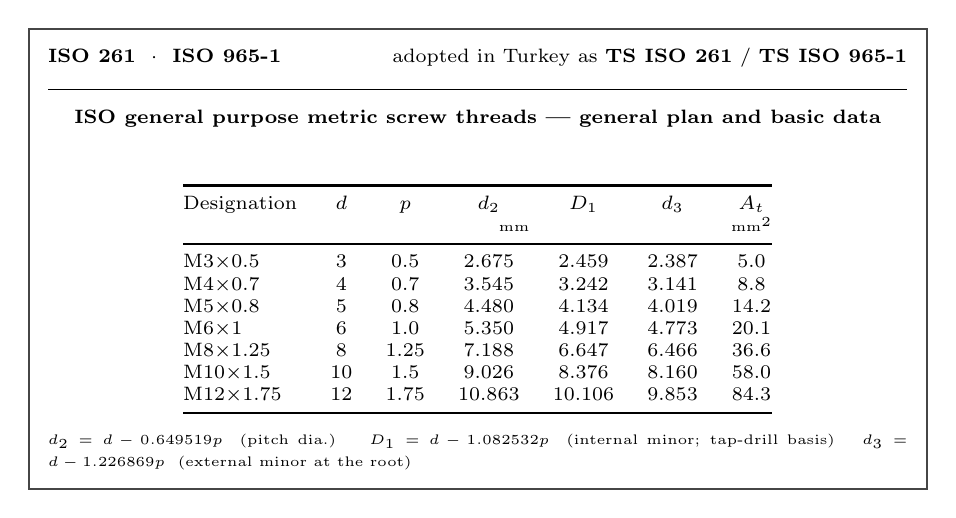
\begin{tikzpicture}
\node[draw=gray!55!black,line width=0.7pt,fill=white,inner sep=7pt,align=left]{%
\begin{minipage}{0.90\textwidth}
\scriptsize
\textbf{ISO 261} \ $\cdot$ \ \textbf{ISO 965-1} \hfill adopted in Turkey as \textbf{TS ISO 261} / \textbf{TS ISO 965-1}\\[2pt]
\rule{\linewidth}{0.6pt}\\[4pt]
\centerline{\textbf{ISO general purpose metric screw threads --- general plan and basic data}}
\vspace{5pt}
\begin{center}
\begin{tabular}{@{}lcccccc@{}}
\toprule
Designation & $d$ & $p$ & $d_2$ & $D_1$ & $d_3$ & $A_t$\\
 & \multicolumn{5}{c}{\tiny mm} & \tiny mm$^2$\\
\midrule
M3$\times$0.5 & 3 & 0.5 & 2.675 & 2.459 & 2.387 & 5.0\\
M4$\times$0.7 & 4 & 0.7 & 3.545 & 3.242 & 3.141 & 8.8\\
M5$\times$0.8 & 5 & 0.8 & 4.480 & 4.134 & 4.019 & 14.2\\
M6$\times$1 & 6 & 1.0 & 5.350 & 4.917 & 4.773 & 20.1\\
M8$\times$1.25 & 8 & 1.25 & 7.188 & 6.647 & 6.466 & 36.6\\
M10$\times$1.5 & 10 & 1.5 & 9.026 & 8.376 & 8.160 & 58.0\\
M12$\times$1.75 & 12 & 1.75 & 10.863 & 10.106 & 9.853 & 84.3\\
\bottomrule
\end{tabular}
\end{center}
\vspace{-2pt}
{\tiny $d_2 = d-0.649519p$ \ (pitch dia.) \quad $D_1 = d-1.082532p$ \ (internal minor; tap-drill basis)
\quad $d_3 = d-1.226869p$ \ (external minor at the root)}
\end{minipage}};
\end{tikzpicture}
\vfill
{\small Every number follows from $p$ and the basic profile. \alert{That is what a dimensional
standard is} --- one geometry, plus the tolerance bands that make parts from different factories fit.}
\end{frame}

\begin{frame}{And the same page in the inch system}
\centering
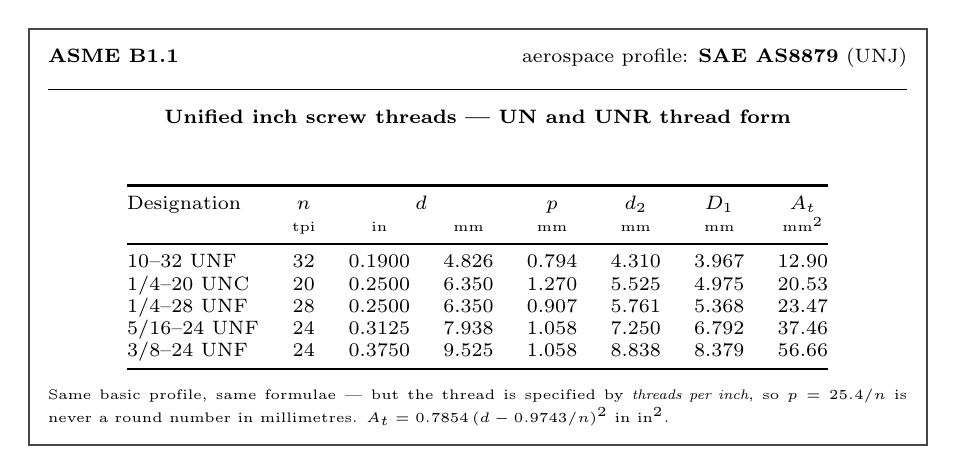
\begin{tikzpicture}
\node[draw=gray!55!black,line width=0.7pt,fill=white,inner sep=7pt,align=left]{%
\begin{minipage}{0.90\textwidth}
\scriptsize
\textbf{ASME B1.1} \hfill aerospace profile: \textbf{SAE AS8879} (UNJ)\\[2pt]
\rule{\linewidth}{0.6pt}\\[4pt]
\centerline{\textbf{Unified inch screw threads --- UN and UNR thread form}}
\vspace{5pt}
\begin{center}
\begin{tabular}{@{}lccccccc@{}}
\toprule
Designation & $n$ & \multicolumn{2}{c}{$d$} & $p$ & $d_2$ & $D_1$ & $A_t$\\
 & \tiny tpi & \tiny in & \tiny mm & \tiny mm & \tiny mm & \tiny mm & \tiny mm$^2$\\
\midrule
10--32 UNF & 32 & 0.1900 & 4.826 & 0.794 & 4.310 & 3.967 & 12.90\\
1/4--20 UNC & 20 & 0.2500 & 6.350 & 1.270 & 5.525 & 4.975 & 20.53\\
1/4--28 UNF & 28 & 0.2500 & 6.350 & 0.907 & 5.761 & 5.368 & 23.47\\
5/16--24 UNF & 24 & 0.3125 & 7.938 & 1.058 & 7.250 & 6.792 & 37.46\\
3/8--24 UNF & 24 & 0.3750 & 9.525 & 1.058 & 8.838 & 8.379 & 56.66\\
\bottomrule
\end{tabular}
\end{center}
\vspace{-2pt}
{\tiny Same basic profile, same formulae --- but the thread is specified by \emph{threads per inch},
so $p = 25.4/n$ is never a round number in millimetres.
$A_t = 0.7854\,(d-0.9743/n)^2$ in \si{in^2}.}
\end{minipage}};
\end{tikzpicture}
\vfill
{\small The geometry is identical --- only the \emph{unit the thread is indexed by} differs, and that
is enough to make the two systems silently incompatible.}
\end{frame}

\begin{frame}{Where this bites: the look-alikes}
\centering\small
\begin{tabular}{@{}llcc@{}}
\toprule
\textbf{Inch} & \textbf{Metric} & $\Delta d$ (\si{mm}) & $\Delta p$ (\si{mm})\\
\midrule
\rowcolor{red!10} 5/16--24 UNF & M8$\times$1 & \alert{\textbf{0.062}} & \alert{\textbf{0.058}}\\
\rowcolor{red!6} 10--32 UNF & M5$\times$0.8 & 0.174 & \alert{\textbf{0.006}}\\
1/4--28 UNF & M6$\times$1 & 0.350 & 0.093\\
3/8--24 UNF & M10$\times$1.25 & 0.475 & 0.192\\
\bottomrule
\end{tabular}
\vfill
\raggedright
A 5/16--24 bolt and an M8$\times$1 hole differ by \SI{62}{\micro\metre} on diameter and
\SI{58}{\micro\metre} on pitch. \alert{It will start. It will feel right. It will take torque.} Then
it will strip, or hold at a fraction of its rated preload.
\vfill
\begin{alertblock}{Why this is a Turkish aerospace problem specifically}
Design and manufacture here run in \textbf{metric} to TS\,/\,EN\,ISO, while much of the airframe
hardware on US-origin aircraft is \textbf{inch} to AN\,/\,MS\,/\,NAS. Both are in the same hangar.\\[4pt]
Segregate the stock, mark the drawings, and never judge a thread by feel.
\end{alertblock}
\end{frame}

\begin{frame}{Property classes --- reading 8.8, 10.9, 12.9}
ISO 898-1 encodes two strengths in one pair of numbers:
\[
\text{first}\times 100 = R_m\ [\si{MPa}],
\qquad
\text{first}\times\text{second}\times 10 = R_e\ [\si{MPa}]
\]
\vfill
\centering\small
\begin{tabular}{@{}lccl@{}}
\toprule
Class & $R_m$ (\si{MPa}) & $R_e$ (\si{MPa}) & \\
\midrule
8.8 & 800 & 640 & general structural\\
10.9 & 1000 & 900 & high-strength\\
12.9 & 1200 & 1080 & highest standard class\\
\bottomrule
\end{tabular}
\vfill
\raggedright
\begin{alertblock}{The strength you cannot simply order more of}
Steels heat-treated much above \SI{1000}{MPa} become susceptible to \textbf{hydrogen embrittlement}
and stress-corrosion cracking. They must be baked after plating to drive the hydrogen out, and the
bake is a process requirement that does not show up on the finished part.\\[4pt]
\alert{Specifying a stronger bolt is not a free upgrade.}
\end{alertblock}
\end{frame}

\begin{frame}{Coarse or fine?}
\centering\small
\begin{tabular}{@{}p{5.1cm}p{5.1cm}@{}}
\toprule
\textbf{Fine} (UNF / UNJF) & \textbf{Coarse} (UNC / metric coarse)\\
\midrule
about \SI{10}{\percent} larger $A_t$ for the same nominal size
  & deeper thread, so more strip area in a soft nut material\\[3pt]
smaller lead angle $\lambda$ --- resists loosening better
  & far more tolerant of damage, corrosion and plating build-up\\[3pt]
finer adjustment per turn
  & faster to assemble, less prone to cross-threading\\[3pt]
shallower thread, easier to damage & coarser adjustment\\
\bottomrule
\end{tabular}
\vfill
\raggedright
\begin{alertblock}{Aerospace practice}
\textbf{Fine} threads in steel and titanium --- which is most airframe hardware, and why you meet UNJF
far more often than UNJC.\\[4pt]
\textbf{Coarse} threads, or a threaded insert, into aluminium and magnesium --- because there the
\emph{internal} thread is the weak member and you need the strip area.
\end{alertblock}
\end{frame}

\begin{frame}{Why the first thread takes so much}
\centering
\resizebox{!}{5.0cm}{
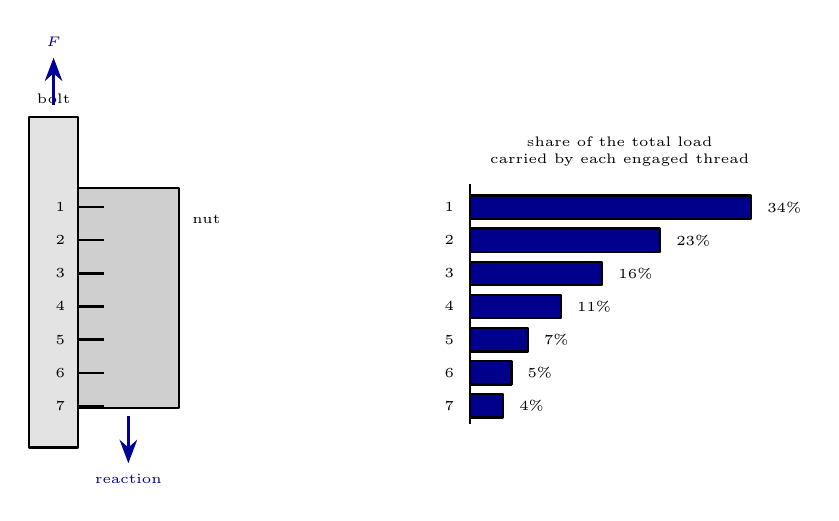
\begin{tikzpicture}[scale=1.0,>=Stealth,font=\scriptsize,line join=round]
% ---------------- left: why ----------------
\begin{scope}
\fill[gray!22] (0,0) rectangle (0.62,4.2);
\draw[thick] (0,0) rectangle (0.62,4.2);
\node[anchor=south,font=\tiny] at (0.31,4.25) {bolt};
\fill[gray!38] (0.62,0.5) rectangle (1.9,3.3);
\draw[thick] (0.62,0.5) rectangle (1.9,3.3);
\node[anchor=west,font=\tiny] at (1.95,2.9) {nut};
\foreach \y/\n in {3.05/1,2.63/2,2.21/3,1.79/4,1.37/5,0.95/6,0.53/7}{
  \draw[thick] (0.62,\y) -- (0.95,\y);
  \node[anchor=east,font=\tiny] at (0.58,\y) {\n};}
\draw[->,blue!60!black,very thick] (0.31,4.35) -- (0.31,4.95);
\node[blue!60!black,anchor=south,font=\tiny] at (0.31,4.97) {$F$};
\draw[->,blue!60!black,very thick] (1.26,0.40) -- (1.26,-0.20);
\node[blue!60!black,anchor=north,font=\tiny,align=center] at (1.26,-0.22) {reaction};
\end{scope}
% ---------------- right: how much ----------------
\begin{scope}[xshift=5.6cm]
\foreach \n/\v in {1/34,2/23,3/16,4/11,5/7,6/5,7/4}{
  \pgfmathsetmacro\yy{3.05-(\n-1)*0.42}
  \pgfmathsetmacro\ww{\v*0.105}
  \fill[blue!55!black] (0,\yy-0.15) rectangle (\ww,\yy+0.15);
  \draw[thick] (0,\yy-0.15) rectangle (\ww,\yy+0.15);
  \node[anchor=west,font=\tiny] at (\ww+0.08,\yy) {\v\%};
  \node[anchor=east,font=\tiny] at (-0.08,\yy) {\n};}
\draw[thick] (0,0.3) -- (0,3.35);
\node[anchor=south,font=\tiny,align=center] at (1.9,3.45)
  {share of the total load\\ carried by each engaged thread};
\end{scope}
\end{tikzpicture}
}
\vfill
\raggedright
{\small This is a \emph{compatibility} result, not a strength result: the bolt and the nut deform in
opposite senses, so the relative displacement that the threads must absorb is concentrated at the
entry. It is why the first thread cracks, why a close class of fit matters, and why a long nut is not
a fix.}
\end{frame}

\section{The aerospace profiles}

\begin{frame}{Start from Lecture 2: the root is a notch}
\[ K_f = 1 + q\,(K_t - 1) \]
\vfill
$K_t$ rises sharply as the root radius falls.
\vfill
A standard UN or ISO metric thread specifies a \emph{maximum} root radius --- or none at all.
\vfill
\begin{alertblock}{So a perfectly sharp root is within specification}
For a part that will see $10^7$ cycles, that is an invitation.
\end{alertblock}
\end{frame}

\begin{frame}{UNJ (AS8879) and MJ (ISO 5855): specify the root}
\centering
\resizebox{0.82\textwidth}{!}{
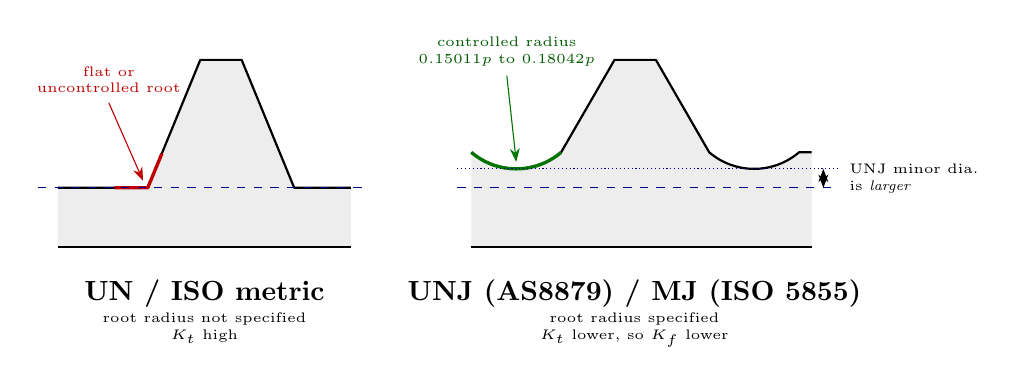
\begin{tikzpicture}[scale=1.5,>=Stealth,font=\scriptsize,line join=round]
\def\hh{1.083}
% ---------------- UN: flat / uncontrolled root ----------------
\begin{scope}
\fill[gray!14] (0.12,0) -- (0.88,0) -- (1.325,\hh) -- (1.675,\hh) -- (2.12,0) -- (2.6,0)
  -- (2.6,-0.5) -- (0.12,-0.5) -- cycle;
\draw[thick] (0.12,0) -- (0.88,0) -- (1.325,\hh) -- (1.675,\hh) -- (2.12,0) -- (2.6,0);
\draw[thick] (0.12,-0.5) -- (2.6,-0.5);
\draw[red!75!black,line width=1.2pt] (0.60,0) -- (0.88,0) -- (1.00,0.29);
\draw[->,red!75!black] (0.55,0.72) -- (0.84,0.06);
\node[red!75!black,anchor=south,align=center,font=\tiny] at (0.55,0.72) {flat or\\ uncontrolled root};
\draw[blue!55!black,dashed] (-0.05,0) -- (2.75,0);
\node[anchor=north,font=\bfseries] at (1.36,-0.70) {UN / ISO metric};
\node[anchor=north,align=center,font=\tiny] at (1.36,-0.98) {root radius not specified\\ $K_t$ high};
\end{scope}
% ---------------- UNJ: controlled root radius ----------------
\begin{scope}[xshift=3.5cm]
\fill[gray!14] (0.12,0.30) arc (229.6:310.4:0.586) -- (1.332,\hh) -- (1.682,\hh)
  -- (2.134,0.30) arc (229.6:310.4:0.586) -- (3.0,0.30) -- (3.0,-0.5) -- (0.12,-0.5) -- cycle;
\draw[thick] (0.12,0.30) arc (229.6:310.4:0.586) -- (1.332,\hh) -- (1.682,\hh)
  -- (2.134,0.30) arc (229.6:310.4:0.586) -- (3.0,0.30);
\draw[thick] (0.12,-0.5) -- (3.0,-0.5);
\draw[green!45!black,line width=1.2pt] (0.12,0.30) arc (229.6:310.4:0.586);
\draw[->,green!45!black] (0.42,0.95) -- (0.50,0.22);
\node[green!35!black,anchor=south,align=center,font=\tiny] at (0.42,0.95)
  {controlled radius\\ $0.15011p$ to $0.18042p$};
\draw[blue!55!black,dashed] (0.0,0) -- (3.22,0);
\draw[blue!55!black,densely dotted] (0.0,0.16) -- (3.22,0.16);
\draw[<->] (3.10,0) -- (3.10,0.16);
\node[anchor=west,font=\tiny,align=left] at (3.24,0.08) {UNJ minor dia.\\ is \emph{larger}};
\node[anchor=north,font=\bfseries] at (1.5,-0.70) {UNJ (AS8879) / MJ (ISO 5855)};
\node[anchor=north,align=center,font=\tiny] at (1.5,-0.98) {root radius specified\\ $K_t$ lower, so $K_f$ lower};
\end{scope}
\end{tikzpicture}
}
\vfill
\[\boxed{\ 0.15011\,p \ \le\ r_{\text{root}} \ \le\ 0.18042\,p\ }\]
\vfill
{\small Minor diameter becomes $d-0.9743p$, not $d-1.0825p$ --- so
\alert{a UNJ bolt and a UN nut are not freely interchangeable}.}
\end{frame}

\begin{frame}{``Why not just specify a good surface finish?''}
A finish callout controls \textbf{roughness} --- a statistical property of the texture.\\[6pt]
$K_t$ depends on \textbf{geometry}.\\[6pt]
Two threads can have identical $R_a$ and differ by a factor of two in root radius.
\vfill
\begin{alertblock}{A caution on the argument you will be tempted to make}
Increasing $r$ lowers $K_t$ --- but it also \emph{raises} $q$ towards 1, which works against you.\\[5pt]
The net effect is still a lower $K_f$, because $K_t$ falls faster than $q$ rises. But the gain is
smaller than a $K_t$ comparison alone suggests.\\[5pt]
\textbf{Quote $K_f$, never $K_t$, when the argument is about fatigue.}
\end{alertblock}
\end{frame}

\begin{frame}{Tensile stress area}
A threaded rod fails on neither the major nor the minor area, but on an empirical area between them.
\begin{columns}[T]
\begin{column}{0.5\textwidth}
\textbf{Unified}
\[ A_t = 0.7854\left(d - \frac{0.9743}{n}\right)^{2} \]
\textbf{ISO metric} (ISO 898-1)
\[ A_t = \frac{\pi}{4}\left(\frac{d_2+d_3}{2}\right)^{2} \]
{\footnotesize $d_2 = d-0.649519p$, \ $d_3 = d-1.226869p$}
\end{column}
\begin{column}{0.46\textwidth}
\centering\small
\begin{tabular}{@{}lS[table-format=2.1]@{}}
\toprule
 & {$A_t$ (\si{mm^2})}\\
\midrule
M6$\times$1 & 20.1\\
M8$\times$1.25 & 36.6\\
M10$\times$1.5 & 58.0\\
1/4--28 UNJF & 23.5\\
5/16--24 UNJF & 37.5\\
\bottomrule
\end{tabular}
\end{column}
\end{columns}
\vfill
{\small Use $A_t$ for tension and preload. For fatigue, use it \emph{and} apply $K_f$ to the
alternating part --- the stress area contains an average allowance for the form, not a notch factor.}
\end{frame}

\begin{frame}{Why $A_t$, and not the root area?}
\centering
\resizebox{!}{3.6cm}{
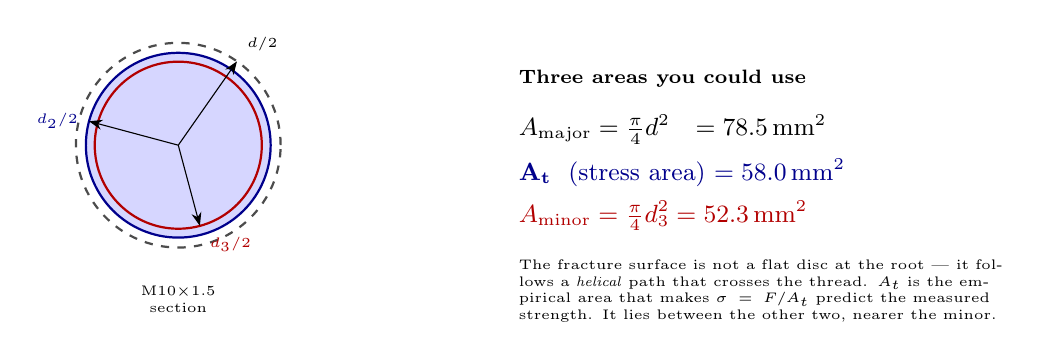
\begin{tikzpicture}[scale=1.0,>=Stealth,font=\scriptsize,line join=round]
% M10 x 1.5 : d=10, d2=9.026, d3=8.160  (radii scaled x0.26)
\def\sc{0.26}
\begin{scope}
\fill[blue!16] (0,0) circle (\sc*4.513);
\draw[thick,dashed,gray!60!black] (0,0) circle (\sc*5.0);
\draw[thick,blue!55!black] (0,0) circle (\sc*4.513);
\draw[thick,red!70!black] (0,0) circle (\sc*4.080);
\draw[->] (0,0) -- (55:\sc*5.0); \node[anchor=south west,font=\tiny] at (55:\sc*5.05) {$d/2$};
\draw[->] (0,0) -- (165:\sc*4.513); \node[anchor=east,font=\tiny,blue!55!black] at (165:\sc*4.6) {$d_2/2$};
\draw[->] (0,0) -- (285:\sc*4.080); \node[anchor=north west,font=\tiny,red!70!black] at (285:\sc*4.15) {$d_3/2$};
\node[anchor=north,align=center,font=\tiny] at (0,-\sc*6.4) {M10$\times$1.5\\ section};
\end{scope}
\begin{scope}[xshift=4.2cm,yshift=-0.1cm]
\node[anchor=west,align=left] at (0,0.95)
 {\textbf{Three areas you could use}};
\node[anchor=west,align=left,font=\small] at (0,0.3)
 {$A_{\text{major}}=\frac{\pi}{4}d^2$ \ \ $=\SI{78.5}{mm^2}$};
\node[anchor=west,align=left,font=\small,blue!55!black] at (0,-0.25)
 {$\mathbf{A_t}$ \ (stress area) $=\SI{58.0}{mm^2}$};
\node[anchor=west,align=left,font=\small,red!70!black] at (0,-0.80)
 {$A_{\text{minor}}=\frac{\pi}{4}d_3^2=\SI{52.3}{mm^2}$};
\node[anchor=west,align=left,font=\tiny,text width=6.4cm] at (0,-1.75)
 {The fracture surface is not a flat disc at the root --- it follows a
  \emph{helical} path that crosses the thread. $A_t$ is the empirical area that
  makes $\sigma = F/A_t$ predict the measured strength. It lies between the
  other two, nearer the minor.};
\end{scope}
\end{tikzpicture}
}
\vfill
\raggedright
{\small Using $A_{\text{minor}}$ is conservative by about \SI{10}{\percent} and using
$A_{\text{major}}$ is dangerously unconservative by about \SI{35}{\percent}. $A_t$ is not a derivation
--- it is a curve fit to test data, and that is exactly why you must use it only for what it was
fitted to: \textbf{static tension and preload}.}
\end{frame}

\begin{frame}{How much thread engagement do you need?}
A threaded joint can fail two ways. \alert{Design so that the bolt breaks in tension, never so that
the threads strip.}
\vfill
\begin{columns}[T]
\begin{column}{0.46\textwidth}
\begin{block}{Why}
A bolt that breaks in tension fails in a way you characterised in Lectures 2--4, at a load you can
compute, in the \emph{replaceable} part.\\[5pt]
A stripped thread is progressive, gives no warning, and destroys the \emph{expensive} part.
\end{block}
\end{column}
\begin{column}{0.50\textwidth}
\begin{block}{Engagement length $L_e$}
\begin{center}\small
\begin{tabular}{@{}ll@{}}
\toprule
Nut material & $L_e$\\
\midrule
steel into steel & $\approx 1.0\,d$\\
into aluminium & $1.5$--$2.0\,d$\\
into magnesium & $2.0$--$2.5\,d$\\
\bottomrule
\end{tabular}
\end{center}
{\footnotesize A standard hex nut is about $0.8\,d$ tall --- sized to make the \emph{bolt} the weak
member.}
\end{block}
\end{column}
\end{columns}
\vfill
{\small Beyond about ten engaged threads the extra ones carry almost nothing --- long enough to be
strip-proof, not so long that you fool yourself.}
\end{frame}

\section{Making the thread}

\begin{frame}{Cut or rolled --- same geometry, different part}
Rolling leaves \textbf{compressive residual stress} at the root, \textbf{work-hardens} the surface, and
leaves the grain flow following the contour instead of cut through it.
\vfill
\centering\small
\begin{tabular}{@{}lcc@{}}
\toprule
$K_f$ for threaded elements & \textbf{Rolled} & \textbf{Cut}\\
\midrule
SAE grade 0--2, metric 3.6--5.8 & 2.2 & 2.8\\
SAE grade 4--8, metric 6.6--10.9 & 3.0 & 3.8\\
\bottomrule
\end{tabular}
\vfill
\raggedright
{\small Source: Shigley, fatigue stress-concentration factors for threaded elements.}
\end{frame}

\begin{frame}{Rolled \emph{after} heat treatment}
\begin{alertblock}{The order matters as much as the process}
Roll, then heat treat $\Rightarrow$ the heat treatment relaxes the compressive residual stress and
\textbf{most of the benefit is lost}.\\[6pt]
Aerospace specifications therefore call for threads \textbf{rolled after heat treatment} --- RAHT.
\end{alertblock}
\vfill
One line on a drawing. Costs almost nothing. Changes the fatigue life by a large factor.
\vfill
\alert{And it is invisible on inspection of the finished part.}
\vfill
{\small Which makes it exactly the requirement that quietly disappears when a part is re-sourced to a
cheaper supplier --- and produces a service failure five years later.}
\end{frame}

\begin{frame}{What the thread form is worth --- Example 5.3}
$1/4$--28 UNJF, $A_t = \SI{23.47}{mm^2}$, $S_e = \SI{160}{MPa}$. \ Allowable alternating stress at the
root is $\sigma_a = S_e/K_f$.
\vfill
\centering
\begin{tabular}{@{}lcc@{}}
\toprule
 & $\sigma_{a,\text{allow}}$ (\si{MPa}) & $F_{a,\text{allow}}$ (\si{N})\\
\midrule
Rolled, $K_f=3.0$ & 53.3 & \textbf{1252}\\
Cut, $K_f=3.8$ & 42.1 & 988\\
\bottomrule
\end{tabular}
\vfill
\raggedright
\textbf{\SI{27}{\percent} more alternating load} for no weight, no material change, essentially no cost.
\vfill
{\small Through the S--N curve, \SI{27}{\percent} on stress is a factor of several on \emph{life}.
Caution: this holds $S_e$ and $A_t$ fixed and changes only $K_f$. It is the size of the prize from the
thread form alone --- not a prediction for a real joint. That is Lecture 6.}
\end{frame}

\begin{frame}{Where the tightening torque goes}
\centering
\resizebox{0.92\textwidth}{!}{
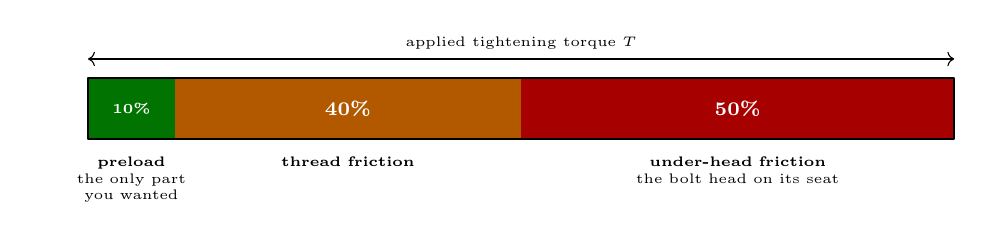
\begin{tikzpicture}[scale=1.0,font=\scriptsize,line join=round]
\def\W{11.0}
\fill[green!45!black] (0,0) rectangle (0.10*\W,0.78);
\fill[orange!70!black] (0.10*\W,0) rectangle (0.50*\W,0.78);
\fill[red!65!black] (0.50*\W,0) rectangle (\W,0.78);
\draw[thick] (0,0) rectangle (\W,0.78);
\node[white,font=\bfseries\tiny] at (0.05*\W,0.39) {10\%};
\node[white,font=\bfseries\scriptsize] at (0.30*\W,0.39) {40\%};
\node[white,font=\bfseries\scriptsize] at (0.75*\W,0.39) {50\%};
\node[anchor=north,align=center,font=\tiny,text width=2.4cm] at (0.05*\W,-0.10)
  {\textbf{preload}\\ the only part you wanted};
\node[anchor=north,align=center,font=\tiny,text width=3.0cm] at (0.30*\W,-0.10)
  {\textbf{thread friction}};
\node[anchor=north,align=center,font=\tiny,text width=3.2cm] at (0.75*\W,-0.10)
  {\textbf{under-head friction}\\ the bolt head on its seat};
\draw[<->] (0,1.02) -- (\W,1.02) node[midway,above,font=\tiny] {applied tightening torque $T$};
\end{tikzpicture}
}
\vfill
\raggedright
You have seen this split before. It is the \textbf{same} split as the power screw's thread and collar
--- and for the same reason: you are turning a screw against friction in two places at once.
\vfill
\begin{alertblock}{The consequence}
About \SI{90}{\percent} of what your torque wrench measures is friction. \alert{Change the friction
and you change the preload, with the torque reading unchanged.}
\end{alertblock}
\end{frame}

\begin{frame}{Stress, strain and stiffness: the joint is two springs}
\begin{columns}[T]
\begin{column}{0.45\textwidth}
Nothing here is new --- it is Hooke's law twice:
\[ \sigma=\frac{F}{A},\quad \varepsilon=\frac{\sigma}{E}=\frac{\delta}{L},
   \quad \delta=\frac{FL}{AE},\quad k=\frac{AE}{L} \]
\vspace{-4pt}
\textbf{The bolt} stretches in \emph{tension} over the grip length. Shank and threaded part act in
series:
\[ \frac{1}{k_b}=\frac{L_s}{A_d E}+\frac{L_t}{A_t E} \]
\textbf{The members} squash in \emph{compression}, over a cone spreading from the head.
\end{column}
\begin{column}{0.52\textwidth}
\begin{block}{M10$\times$1.5 through \SI{30}{mm} of steel}
\small
$A_d = \SI{78.5}{mm^2}$, \ $A_t = \SI{58.0}{mm^2}$, \ $E = \SI{207}{GPa}$
\[ k_b = \SI{485}{kN/mm} \qquad k_m = \SI{1936}{kN/mm} \]
\[ \frac{k_m}{k_b} = 4.0
   \qquad\Rightarrow\qquad
   \boxed{\,C=\frac{k_b}{k_b+k_m}=0.20\,} \]
\end{block}
\centering
\alert{The bolt takes only \SI{20}{\percent} of any external load.}\\
The members shed the other \SI{80}{\percent}.
\end{column}
\end{columns}
\end{frame}

\begin{frame}{The stress cone --- where the clamp actually goes}
\centering
\resizebox{!}{3.4cm}{
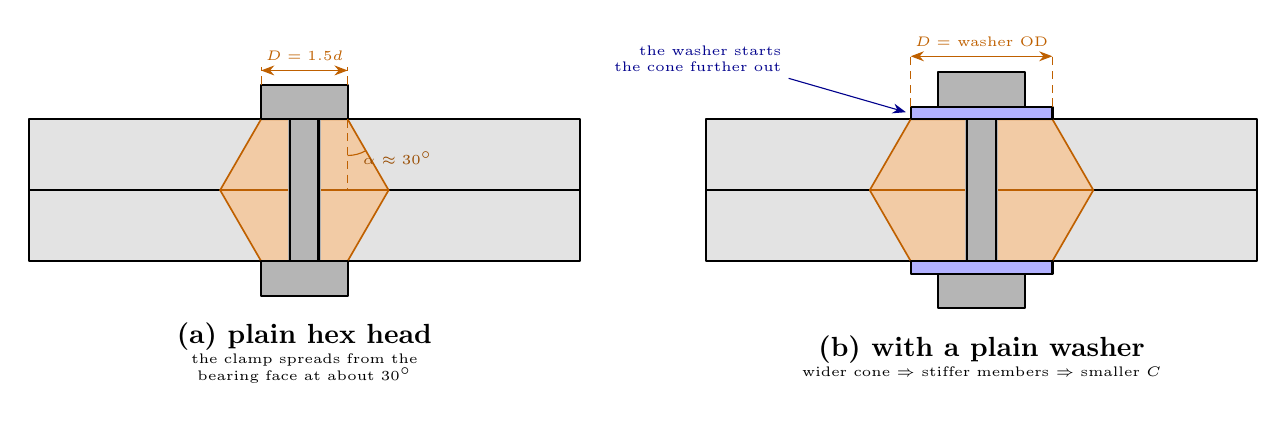
\begin{tikzpicture}[scale=1.0,>=Stealth,font=\scriptsize,line join=round]
\tikzset{pl/.style={thick,fill=gray!22},bl/.style={thick,fill=gray!58},
         wsh/.style={thick,fill=blue!30},
         cone/.style={fill=orange!55,fill opacity=0.55,draw=orange!75!black,line width=0.6pt}}
%============ (a) bare head ============
\begin{scope}
\draw[pl] (0,0) rectangle (7,0.90);
\draw[pl] (0,-0.90) rectangle (7,0);
\fill[cone] (2.95,0.90) -- (2.43,0) -- (4.57,0) -- (4.05,0.90) -- cycle;
\fill[cone] (2.95,-0.90) -- (2.43,0) -- (4.57,0) -- (4.05,-0.90) -- cycle;
\fill[white] (3.30,-0.90) rectangle (3.70,0.90);
\draw[gray!60] (3.30,-0.90) -- (3.30,0.90); \draw[gray!60] (3.70,-0.90) -- (3.70,0.90);
\draw[bl] (3.32,-1.34) rectangle (3.68,1.34);
\draw[bl] (2.95,0.90) rectangle (4.05,1.34);
\draw[bl] (2.95,-1.34) rectangle (4.05,-0.90);
\draw[<->,orange!75!black] (2.95,1.52) -- (4.05,1.52) node[midway,above,font=\tiny]{$D=1.5d$};
\draw[orange!75!black,densely dashed] (2.95,1.34) -- (2.95,1.56);
\draw[orange!75!black,densely dashed] (4.05,1.34) -- (4.05,1.56);
\draw[orange!75!black,densely dashed] (4.05,0.90) -- (4.05,0.02);
\draw[orange!75!black] (4.05,0.44) arc (270:300:0.46);
\node[orange!60!black,anchor=west,font=\tiny] at (4.12,0.40) {$\alpha\approx\SI{30}{\degree}$};
\node[anchor=north,font=\bfseries] at (3.5,-1.56) {(a) plain hex head};
\node[anchor=north,align=center,font=\tiny,text width=4.2cm] at (3.5,-1.96)
  {the clamp spreads from the bearing face at about \SI{30}{\degree}};
\end{scope}
%============ (b) with a washer ============
\begin{scope}[xshift=8.6cm]
\draw[pl] (0,0) rectangle (7,0.90);
\draw[pl] (0,-0.90) rectangle (7,0);
\fill[cone] (2.60,0.90) -- (2.08,0) -- (4.92,0) -- (4.40,0.90) -- cycle;
\fill[cone] (2.60,-0.90) -- (2.08,0) -- (4.92,0) -- (4.40,-0.90) -- cycle;
\fill[white] (3.30,-0.90) rectangle (3.70,0.90);
\draw[gray!60] (3.30,-0.90) -- (3.30,0.90); \draw[gray!60] (3.70,-0.90) -- (3.70,0.90);
\draw[bl] (3.32,-1.50) rectangle (3.68,1.50);
\draw[wsh] (2.60,0.90) rectangle (4.40,1.06);
\draw[wsh] (2.60,-1.06) rectangle (4.40,-0.90);
\draw[bl] (2.95,1.06) rectangle (4.05,1.50);
\draw[bl] (2.95,-1.50) rectangle (4.05,-1.06);
\draw[<->,orange!75!black] (2.60,1.70) -- (4.40,1.70) node[midway,above,font=\tiny]{$D=$ washer OD};
\draw[orange!75!black,densely dashed] (2.60,1.06) -- (2.60,1.74);
\draw[orange!75!black,densely dashed] (4.40,1.06) -- (4.40,1.74);
\draw[->,blue!55!black] (1.05,1.42) -- (2.54,0.99);
\node[blue!55!black,anchor=south east,align=right,font=\tiny,text width=2.2cm] at (1.08,1.38)
  {the washer starts the cone further out};
\node[anchor=north,font=\bfseries] at (3.5,-1.72) {(b) with a plain washer};
\node[anchor=north,align=center,font=\tiny,text width=4.8cm] at (3.5,-2.12)
  {wider cone $\Rightarrow$ stiffer members $\Rightarrow$ smaller $C$};
\end{scope}
\end{tikzpicture}
}
\vfill
\raggedright
The members are \emph{not} uniformly compressed. The clamp spreads out from the bearing face into a
cone --- the R\"otscher cone --- with a half-angle of about \SI{30}{\degree}. \alert{$k_m$ is simply
the stiffness of two truncated cones in series}, which is why its formula looks so unlike $AE/L$.
\end{frame}

\begin{frame}{Three things the cone decides for you}
\begin{enumerate}
  \item \textbf{What is actually clamped.} Only the material inside the cone is held together.
        Outside it the joint is not clamped at all --- which is what sets the \emph{maximum bolt
        spacing} in a pressure joint or a flange.
  \item \textbf{Whether the cone fits in the part.} Too little edge distance, or too thin a boss, and
        the cone runs out of the side of the material. The clamped volume collapses, $k_m$ falls, and
        $C$ rises --- the bolt starts taking the external load it was meant to be shielded from.
  \item \textbf{Where the cone starts.} The cone begins at the \emph{bearing face} diameter. Change
        that diameter and you change $k_m$.
\end{enumerate}
\vfill
\begin{alertblock}{And item 3 is a washer}
That is the structural job of a plain washer --- not packing, not protection. \alert{It is a
stiffness device.}
\end{alertblock}
\end{frame}

\begin{frame}{What a washer is worth --- the same M10 joint}
\centering\small
\begin{tabular}{@{}lcccc@{}}
\toprule
Bearing face & $k_m$ (\si{kN/mm}) & $C=\frac{k_b}{k_b+k_m}$ & $\sigma_a$ rel. & under-head $\sigma_b$\\
\midrule
bare hex head, $D=1.5d$ & 1936 & 0.200 & 1.00 & \SI{401}{MPa}\\
plain washer, OD $2.0d$ & 3417 & \alert{\textbf{0.124}} & \alert{\textbf{0.62}} & \alert{\SI{159}{MPa}}\\
large washer, OD $2.4d$ & 4771 & 0.092 & 0.46 & \SI{99}{MPa}\\
\bottomrule
\end{tabular}
\vfill
\raggedright
\begin{columns}[T]
\begin{column}{0.47\textwidth}
\begin{block}{\small As a stiffness device}
\footnotesize A plain washer cuts the bolt's share of the external load from \SI{20}{\percent} to
\SI{12}{\percent} --- a \SI{38}{\percent} reduction in alternating stress, for the price of a washer.
\end{block}
\end{column}
\begin{column}{0.47\textwidth}
\begin{block}{\small As a bearing pad}
\footnotesize \SI{401}{MPa} under a bare head at \SI{36}{kN} preload will \emph{embed} into an
aluminium member. Embedment is local yielding at the interface --- and it shows up later as
\alert{lost preload}.
\end{block}
\end{column}
\end{columns}
\end{frame}

\begin{frame}{Washers are not all one thing}
\centering
\resizebox{0.99\textwidth}{!}{
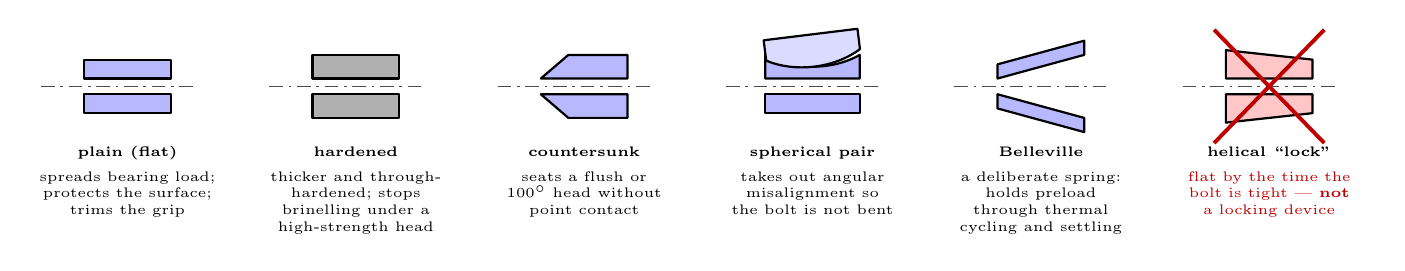
\begin{tikzpicture}[scale=1.0,>=Stealth,font=\scriptsize,line join=round]
\tikzset{w/.style={thick,fill=blue!28},ax/.style={dash pattern=on 5pt off 2pt on 1pt off 2pt,gray!60!black,line width=0.3pt}}
\def\panel#1#2{\node[anchor=north,font=\bfseries\tiny] at (#1,-0.64) {#2};}
% 1 plain
\begin{scope}
\draw[ax] (-0.1,0) -- (1.9,0);
\draw[w] (0.45,0.10) rectangle (1.55,0.34);
\draw[w] (0.45,-0.34) rectangle (1.55,-0.10);
\panel{1.0}{plain (flat)}
\node[anchor=north,align=center,font=\tiny,text width=2.3cm] at (1.0,-0.96)
  {spreads bearing load; protects the surface; trims the grip};
\end{scope}
% 2 hardened / structural
\begin{scope}[xshift=2.9cm]
\draw[ax] (-0.1,0) -- (1.9,0);
\draw[thick,fill=gray!62] (0.45,0.10) rectangle (1.55,0.40);
\draw[thick,fill=gray!62] (0.45,-0.40) rectangle (1.55,-0.10);
\panel{1.0}{hardened}
\node[anchor=north,align=center,font=\tiny,text width=2.3cm] at (1.0,-0.96)
  {thicker and through-hardened; stops brinelling under a high-strength head};
\end{scope}
% 3 countersunk
\begin{scope}[xshift=5.8cm]
\draw[ax] (-0.1,0) -- (1.9,0);
\draw[w] (0.45,0.10) -- (1.55,0.10) -- (1.55,0.40) -- (0.80,0.40) -- cycle;
\draw[w] (0.45,-0.10) -- (1.55,-0.10) -- (1.55,-0.40) -- (0.80,-0.40) -- cycle;
\panel{1.0}{countersunk}
\node[anchor=north,align=center,font=\tiny,text width=2.3cm] at (1.0,-0.96)
  {seats a flush or \SI{100}{\degree} head without point contact};
\end{scope}
% 4 spherical pair
\begin{scope}[xshift=8.7cm]
\draw[ax] (-0.1,0) -- (1.9,0);
% lower washer: flat base, concave spherical seat on top
\draw[w] (0.40,0.10) -- (1.60,0.10) -- (1.60,0.40)
  .. controls (1.25,0.20) and (0.75,0.20) .. (0.40,0.40) -- cycle;
% upper washer: convex spherical underside, tilted to show it self-aligns
\draw[thick,fill=blue!14,rotate around={7:(1.0,0.46)}]
  (0.40,0.40) .. controls (0.75,0.20) and (1.25,0.20) .. (1.60,0.40)
  -- (1.60,0.66) -- (0.40,0.66) -- cycle;
\draw[w] (0.40,-0.10) rectangle (1.60,-0.34);
\panel{1.0}{spherical pair}
\node[anchor=north,align=center,font=\tiny,text width=2.4cm] at (1.0,-0.96)
  {takes out angular misalignment so the bolt is not bent};
\end{scope}
% 5 Belleville
\begin{scope}[xshift=11.6cm]
\draw[ax] (-0.1,0) -- (1.9,0);
\draw[w] (0.45,0.10) -- (1.55,0.40) -- (1.55,0.58) -- (0.45,0.28) -- cycle;
\draw[w] (0.45,-0.28) -- (1.55,-0.58) -- (1.55,-0.40) -- (0.45,-0.10) -- cycle;
\panel{1.0}{Belleville}
\node[anchor=north,align=center,font=\tiny,text width=2.4cm] at (1.0,-0.96)
  {a deliberate spring: holds preload through thermal cycling and settling};
\end{scope}
% 6 helical spring "lock" washer
\begin{scope}[xshift=14.5cm]
\draw[ax] (-0.1,0) -- (1.9,0);
\draw[thick,fill=red!22] (0.45,0.10) -- (1.55,0.10) -- (1.55,0.34) -- (0.45,0.46) -- cycle;
\draw[thick,fill=red!22] (0.45,-0.46) -- (1.55,-0.34) -- (1.55,-0.10) -- (0.45,-0.10) -- cycle;
\draw[red!75!black,line width=1.4pt] (0.30,0.72) -- (1.70,-0.72);
\draw[red!75!black,line width=1.4pt] (1.70,0.72) -- (0.30,-0.72);
\panel{1.0}{helical ``lock''}
\node[anchor=north,align=center,font=\tiny,text width=2.5cm,red!75!black] at (1.0,-0.96)
  {flat by the time the bolt is tight --- \textbf{not} a locking device};
\end{scope}
\end{tikzpicture}
}
\vfill
\raggedright
\begin{alertblock}{On the last one --- NASA's fastener design manual, RP-1228}
``The lockwasher serves as a spring while the bolt is being tightened. However, the washer is normally
flat by the time the bolt is fully torqued. \alert{In summary, a lockwasher of this type is useless
for locking.}''
\end{alertblock}
\vfill
{\small In aerospace, locking is \textbf{positive}: safety wire, a cotter pin through a castellated
nut, or a self-locking nut with a specified run-on torque. Never a spring washer, and never friction
alone.}
\end{frame}

\begin{frame}{Choosing the preload}
\centering
\resizebox{!}{3.3cm}{
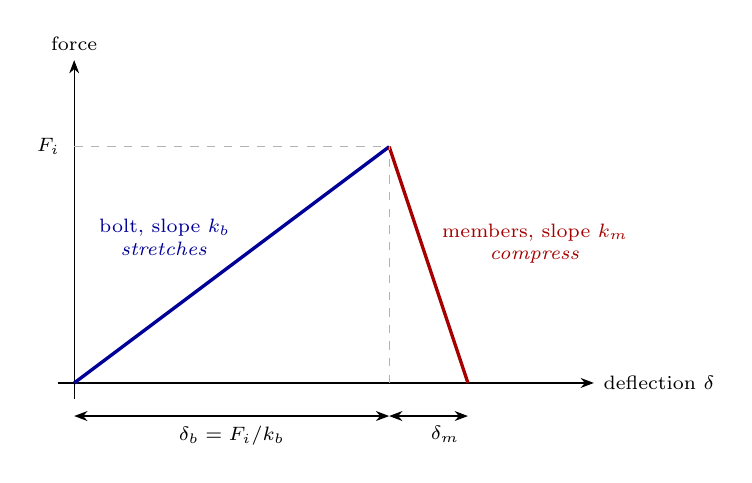
\begin{tikzpicture}[scale=1.0,>=Stealth,font=\scriptsize,line join=round]
\draw[->] (-0.2,0) -- (6.6,0) node[right] {deflection $\delta$};
\draw[->] (0,-0.2) -- (0,4.1) node[above] {force};
% bolt line (shallow, slope k_b) and member line (steep, slope k_m)
\draw[very thick,blue!60!black] (0,0) -- (4,3);
\draw[very thick,red!65!black] (5,0) -- (4,3);
\draw[gray!60,dashed] (0,3) -- (4,3);
\draw[gray!60,dashed] (4,0) -- (4,3);
\node[anchor=east] at (-0.06,3) {$F_i$};
\node[blue!60!black,anchor=south east,align=center] at (2.1,1.5)
  {bolt, slope $k_b$\\ \emph{stretches}};
\node[red!65!black,anchor=south west,align=center] at (4.55,1.4)
  {members, slope $k_m$\\ \emph{compress}};
\draw[<->] (0,-0.42) -- (4,-0.42) node[midway,below] {$\delta_b = F_i/k_b$};
\draw[<->] (4,-0.42) -- (5,-0.42) node[midway,below,xshift=6pt] {$\delta_m$};
\end{tikzpicture}
}
\vfill
\raggedright
\begin{columns}[T]
\begin{column}{0.44\textwidth}
\begin{block}{The rule}
\small
\[ F_p = A_t S_p, \qquad
   F_i = \begin{cases} 0.75\,F_p & \text{reused} \\ 0.90\,F_p & \text{permanent}\end{cases} \]
\vspace{-6pt}
{\footnotesize $S_p$ is the \emph{proof stress}: \SI{830}{MPa} for class 10.9.}
\end{block}
\end{column}
\begin{column}{0.52\textwidth}
\begin{block}{M10$\times$1.5, class 10.9}
\small
$F_p = 58.0\times830 = \SI{48.1}{kN}$\\[3pt]
$F_i = 0.75\times48.1 = \mathbf{\SI{36.1}{kN}}$
\end{block}
\end{column}
\end{columns}
\end{frame}

\begin{frame}{What that preload buys you}
Take the same joint, $C=0.20$, and apply an external load cycling from 0 to \SI{10}{kN}.
\vfill
\centering\small
\begin{tabular}{@{}lcc@{}}
\toprule
 & bolt load range & $\sigma_a$ at the thread root\\
\midrule
No preload --- bolt takes all of $P$ & \SIrange{0}{10}{kN} & \SI{86.2}{MPa}\\
Preloaded --- bolt takes $C\,P$ & $36.1 \to \SI{38.1}{kN}$ & \alert{\textbf{\SI{17.3}{MPa}}}\\
\bottomrule
\end{tabular}
\vfill
\raggedright
A factor of \textbf{five} on the alternating stress --- and through the S--N curve, far more than a
factor of five on life.
\vfill
\begin{alertblock}{This is the whole reason a bolt is tightened}
Not to stop it falling out. \alert{Preload exists to keep the external load off the bolt}, by holding
the joint closed so the stiff members absorb most of it. A loose bolt in a cyclically loaded joint is
not a slightly worse joint --- it is a fatigue failure with a date on it.
\end{alertblock}
\vfill
{\small The full external-load analysis, and what happens when the joint separates, is Lecture 6.}
\end{frame}

\begin{frame}{From preload to tightening torque}
You cannot measure \SI{36.1}{kN} with a spanner. You measure torque, through the nut factor:
\[ \boxed{\;T = K\,d\,F_i\;} \]
\vfill
\centering\small
\begin{tabular}{@{}lcc@{}}
\toprule
M10$\times$1.5, class 10.9, $F_i=\SI{36.1}{kN}$ & $K$ & $T$\\
\midrule
dry, as-received & 0.20 & \SI{72.2}{N.m}\\
lubricated & 0.15 & \SI{54.1}{N.m}\\
\bottomrule
\end{tabular}
\vfill
\raggedright
\begin{alertblock}{Now take the dry value and lubricate the bolt}
Same wrench, same \SI{72.2}{N.m}, but $K$ has fallen to 0.15:
\[ F_i = \frac{T}{K d} = \frac{72.2}{0.15\times0.010} = \SI{48.1}{kN}
   = \mathbf{100\%\ \text{of the proof load}} \]
\alert{A squirt of oil has taken the bolt from \SI{75}{\percent} of proof to its proof load, with the
torque unchanged and nothing to see.}
\end{alertblock}
\end{frame}

\begin{frame}{Why torque is a poor way to set preload}
The nut factor $K$ lumps all of that friction into one number:
\[
\boxed{\;T = K\,d\,F_i\;}\qquad K \approx 0.20 \ \text{dry}, \qquad K \approx 0.15 \ \text{lubricated}
\]
\vfill
Torque control delivers the intended preload to about \alert{$\pm\SI{25}{\percent}$ to
$\pm\SI{35}{\percent}$}. That scatter is not poor workmanship --- it is the method.
\vfill
\begin{columns}[T]
\begin{column}{0.46\textwidth}
\textbf{Better, in increasing accuracy}
\begin{itemize}\footnotesize
  \item turn-of-nut
  \item measured bolt elongation
  \item ultrasonic length measurement
  \item load-indicating washers
\end{itemize}
\end{column}
\begin{column}{0.50\textwidth}
\begin{alertblock}{\small Why aerospace torque values read the way they do}
\footnotesize The \emph{run-on} torque of a self-locking nut must be measured and \textbf{added} to
the specified value; a re-used nut has a different one; and a lubricant changes $K$ outright. That is
why a torque is always quoted with its exact lubrication and locking condition.
\end{alertblock}
\end{column}
\end{columns}
\end{frame}

\section{Heads, drives and countersinks}

\begin{frame}{The head is not a handle}
Three jobs, and a drawing has to settle all three.
\vfill
\begin{columns}[T]
\begin{column}{0.32\textwidth}
\begin{block}{1. Spread the preload}
Enough bearing area that the member does not \textbf{embed}.
\end{block}
\end{column}
\begin{column}{0.32\textwidth}
\begin{block}{2. Take the tool}
A drive that will not round out at the torque you specified.
\end{block}
\end{column}
\begin{column}{0.32\textwidth}
\begin{block}{3. Be the surface}
On a flush fastener the head \emph{is} outer mould line.
\end{block}
\end{column}
\end{columns}
\vfill
\begin{alertblock}{And under the head, a fillet}
It carries the \textbf{whole} bolt tension across a change of section --- the second place a
tension bolt cracks, after the first engaged thread.
\begin{itemize}
\item Never machine it off. If the head will not seat, the \textbf{hole} is wrong.
\item The hole chamfer must \textbf{clear} it, or the head bears on a line.
\item A washer goes \textbf{chamfered face towards the head} --- upside down its sharp corner bears into the fillet, and nobody can see it afterwards.
\end{itemize}
\end{alertblock}
\end{frame}

\begin{frame}{Protruding heads}
\centering
\resizebox{!}{3.4cm}{% Head types in elevation. Common shank diameter d = 1.
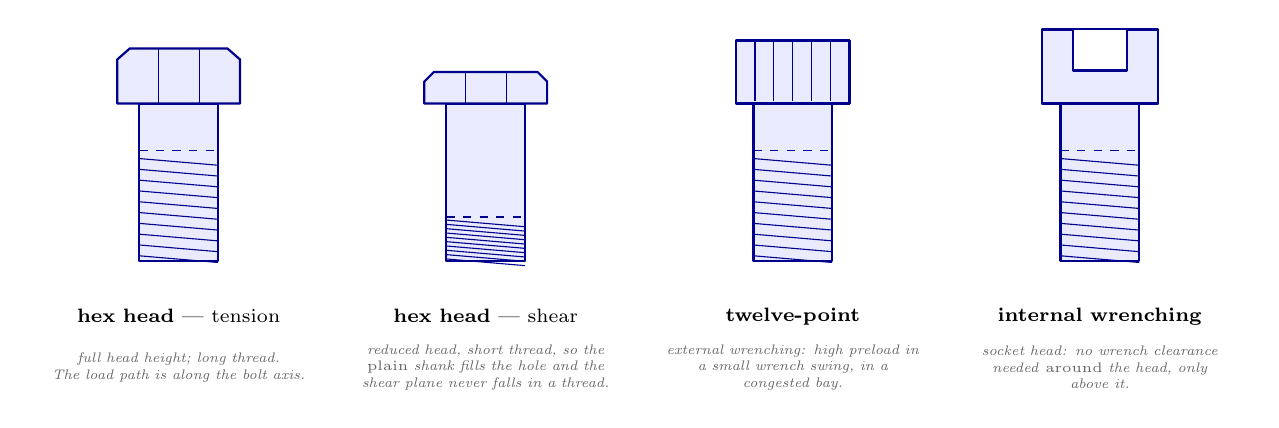
\begin{tikzpicture}[>=Latex,line join=round]
\tikzset{
  steel/.style={fill=blue!8,draw=blue!55!black,thick},
  lbl/.style={font=\scriptsize,align=center,text width=3.6cm},
  sub/.style={font=\tiny\itshape,align=center,text width=3.6cm,text=black!60},
  dimn/.style={<->,gray!80!black,thin},
  note/.style={font=\tiny,text=red!65!black,align=center,text width=2.9cm}
}

% \shank{x centre}{total length}{fraction of length that is plain shank}
\newcommand{\shank}[3]{%
  \draw[steel] (#1-0.5,0) rectangle (#1+0.5,-#2);
  \foreach \k in {0,1,...,9}{%
    \pgfmathsetmacro\yy{-#2*(#3+(1-#3)*(0.07+0.098*\k))}
    \ifdim\yy pt>-#2 pt
      \draw[blue!55!black,thin] (#1-0.5,\yy) -- (#1+0.5,\yy-0.085);
    \fi}
  \draw[blue!55!black,thin,dashed] (#1-0.5,-#2*#3) -- (#1+0.5,-#2*#3);
}

%==================== ROW 1 : protruding heads ====================
\begin{scope}

% --- 1. hex head, tension ---
\def\x{0}
\shank{\x}{2.00}{0.30}
\fill[blue!8,draw=blue!55!black,thick]
  (\x-0.78,0) -- (\x+0.78,0) -- (\x+0.78,0.56) -- (\x+0.62,0.70)
  -- (\x-0.62,0.70) -- (\x-0.78,0.56) -- cycle;
\draw[blue!55!black] (\x-0.26,0) -- (\x-0.26,0.70);
\draw[blue!55!black] (\x+0.26,0) -- (\x+0.26,0.70);
\node[lbl] at (\x,-2.70) {\textbf{hex head} --- tension};
\node[sub] at (\x,-3.35) {full head height; long thread.\\ The load path is along the bolt axis.};

% --- 2. hex head, shear ---
\def\x{3.9}
\shank{\x}{2.00}{0.72}
\fill[blue!8,draw=blue!55!black,thick]
  (\x-0.78,0) -- (\x+0.78,0) -- (\x+0.78,0.28) -- (\x+0.66,0.40)
  -- (\x-0.66,0.40) -- (\x-0.78,0.28) -- cycle;
\draw[blue!55!black] (\x-0.26,0) -- (\x-0.26,0.40);
\draw[blue!55!black] (\x+0.26,0) -- (\x+0.26,0.40);
\node[lbl] at (\x,-2.70) {\textbf{hex head} --- shear};
\node[sub] at (\x,-3.35) {reduced head, short thread, so the\\ \emph{plain} shank fills the hole and the\\ shear plane never falls in a thread.};

% --- 3. twelve-point external wrenching ---
\def\x{7.8}
\shank{\x}{2.00}{0.30}
\fill[blue!8,draw=blue!55!black,thick]
  (\x-0.72,0) -- (\x+0.72,0) -- (\x+0.72,0.80) -- (\x-0.72,0.80) -- cycle;
\foreach \k in {-0.48,-0.24,0,0.24,0.48}{
  \draw[blue!55!black,thin] (\x+\k,0.03) -- (\x+\k,0.80);}
\node[lbl] at (\x,-2.70) {\textbf{twelve-point}};
\node[sub] at (\x,-3.35) {external wrenching: high preload in\\ a small wrench swing, in a\\ congested bay.};

% --- 4. internal wrenching / socket cap ---
\def\x{11.7}
\shank{\x}{2.00}{0.30}
\fill[blue!8,draw=blue!55!black,thick]
  (\x-0.74,0) -- (\x+0.74,0) -- (\x+0.74,0.94) -- (\x-0.74,0.94) -- cycle;
\fill[white,draw=blue!55!black,thick]
  (\x-0.34,0.95) -- (\x-0.34,0.42) -- (\x+0.34,0.42) -- (\x+0.34,0.95) -- cycle;
\node[lbl] at (\x,-2.70) {\textbf{internal wrenching}};
\node[sub] at (\x,-3.35) {socket head: no wrench clearance\\ needed \emph{around} the head, only\\ above it.};

\end{scope}

\end{tikzpicture}
}
\vfill
\raggedright\footnotesize
\begin{tabular}{@{}lll@{}}
\toprule
Head & Standard & What it is for\\
\midrule
Hexagon & ISO 4014 / 4017 & general-purpose; needs swing room \emph{around} the head\\
Hexagon socket cap & ISO 4762 & no room beside the head, only above it\\
Hexagon socket countersunk & ISO 10642 ($90^\circ$) & flush, in machinery\\
Button / dome & ISO 7380 & low head, light duty --- not structural\\
Twelve-point external & NAS624--644 & high preload in a small wrench swing\\
Flanged & ISO 4162 & integral bearing flange, replaces a washer\\
\bottomrule
\end{tabular}
\end{frame}

\begin{frame}{The bolt tells you what it is}
\begin{columns}[T]
\begin{column}{0.46\textwidth}
\textbf{Aerospace families}
\vspace{2pt}
{\footnotesize
\begin{tabular}{@{}ll@{}}
\toprule
AN3--AN20 & hex head, structural\\
AN21--AN36 & clevis --- \alert{shear only}\\
AN42--AN49 & eyebolt --- external tension\\
AN73--AN81 & drilled head, for lockwire\\
NAS144--158 & internal wrenching, tension\\
NAS624--644 & twelve-point external\\
NAS333--340 & $100^\circ$ countersunk, close tol.\\
\bottomrule
\end{tabular}}
\end{column}
\begin{column}{0.50\textwidth}
\textbf{Head markings} {\scriptsize(FAA AC 43.13-1B \S7-36)}
\vspace{2pt}
{\footnotesize
\begin{tabular}{@{}ll@{}}
\toprule
raised dash / asterisk & AN standard steel\\
single dash & corrosion-resistant steel\\
two raised dashes & aluminium alloy\\
triangle & close-tolerance NAS\\
\alert{nothing at all} & \alert{low-strength commercial}\\
\bottomrule
\end{tabular}}

\vspace{4pt}

{\scriptsize An unmarked bolt in a structure is a \textbf{finding}, not a puzzle. Reading heads is
the cheapest inspection there is --- it needs no equipment.}
\end{column}
\end{columns}
\end{frame}

\begin{frame}{Shear head or tension head?}
Same diameter, same alloy, same heat treatment --- and \alert{not interchangeable}.
\vfill
\centering\small
\begin{tabular}{@{}lll@{}}
\toprule
 & \textbf{Tension bolt} & \textbf{Shear bolt}\\
\midrule
Head height & full & reduced\\
Thread length & long & short\\
What fills the hole & thread may reach it & the \textbf{plain shank}\\
Carries & axial tension & transverse shear\\
Example & NAS6203 & NAS6603\\
\bottomrule
\end{tabular}
\vfill
\raggedright
\begin{alertblock}{Why the short thread matters}
If a \textbf{thread} lies in the shear plane, the resisting area is $A_t$, not $\pi d^2/4$ --- and the
thread root is a notch sitting exactly where the bearing stress peaks.
\vspace{2pt}
So \textbf{grip length is a design dimension}: long enough that the run-out clears the shear plane,
short enough that the head still seats on the member.
\end{alertblock}
\end{frame}

\begin{frame}{Flush, and the angle that goes with it}
A protruding head stands in the boundary layer. One is nothing; a few hundred thousand over the
wetted area are not --- and on a military aircraft each one is a radar return.
\vfill
\centering\small
\begin{tabular}{@{}llc@{}}
\toprule
Included angle & Where & Standard\\
\midrule
\textbf{$100^\circ$} & \textbf{aerospace} --- bolts, screws, solid rivets & AN/MS/NAS\\
$90^\circ$ & metric general engineering & ISO 10642\\
$82^\circ$ & inch commercial (US) & ASME B18.3\\
\bottomrule
\end{tabular}
\vfill
\raggedright
\begin{alertblock}{The head angle and the countersink angle must be the same number}
$82^\circ$ head in a $100^\circ$ hole: touches at the \textbf{rim} only.
$100^\circ$ head in an $82^\circ$ hole: touches at the \textbf{bottom edge} only.
\vspace{2pt}
Either way the annular bearing area becomes a line --- and neither is visible once the fastener is
driven. This is the strongest argument there is against mixing inch and metric hardware.
\end{alertblock}
\end{frame}

\begin{frame}{How deep may the countersink go?}
\centering
\resizebox{!}{3.5cm}{% Head types in elevation. Common shank diameter d = 1.
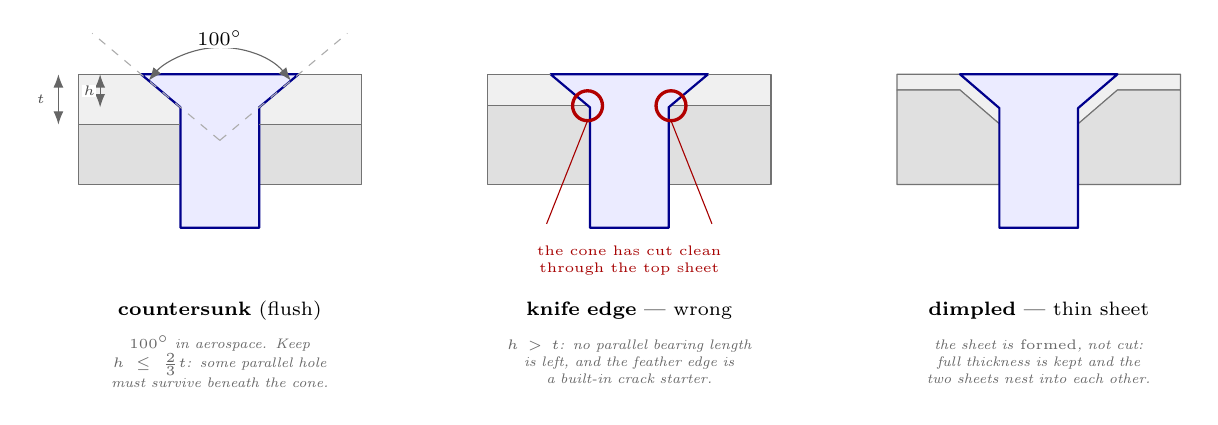
\begin{tikzpicture}[>=Latex,line join=round]
\tikzset{
  steel/.style={fill=blue!8,draw=blue!55!black,thick},
  lbl/.style={font=\scriptsize,align=center,text width=3.6cm},
  sub/.style={font=\tiny\itshape,align=center,text width=3.6cm,text=black!60},
  dimn/.style={<->,gray!80!black,thin},
  note/.style={font=\tiny,text=red!65!black,align=center,text width=2.9cm}
}

% \shank{x centre}{total length}{fraction of length that is plain shank}
\newcommand{\shank}[3]{%
  \draw[steel] (#1-0.5,0) rectangle (#1+0.5,-#2);
  \foreach \k in {0,1,...,9}{%
    \pgfmathsetmacro\yy{-#2*(#3+(1-#3)*(0.07+0.098*\k))}
    \ifdim\yy pt>-#2 pt
      \draw[blue!55!black,thin] (#1-0.5,\yy) -- (#1+0.5,\yy-0.085);
    \fi}
  \draw[blue!55!black,thin,dashed] (#1-0.5,-#2*#3) -- (#1+0.5,-#2*#3);
}

%==================== ROW 2 : flush heads and the countersink ====================
\begin{scope}

% --- 5. 100 deg countersunk, correct ---
\def\x{0}
\fill[black!6,draw=black!55] (\x-1.80,0) rectangle (\x+1.80,-0.64);
\fill[black!12,draw=black!55] (\x-1.80,-0.64) rectangle (\x+1.80,-1.40);
\fill[white] (\x-1.00,0.01) -- (\x-0.5,-0.42) -- (\x-0.5,-1.41) -- (\x+0.5,-1.41)
   -- (\x+0.5,-0.42) -- (\x+1.00,0.01) -- cycle;
\fill[blue!8,draw=blue!55!black,thick]
  (\x-1.00,0) -- (\x+1.00,0) -- (\x+0.5,-0.42) -- (\x+0.5,-1.95)
  -- (\x-0.5,-1.95) -- (\x-0.5,-0.42) -- cycle;
\draw[black!55] (\x-1.80,0) -- (\x-1.00,0);  \draw[black!55] (\x+1.00,0) -- (\x+1.80,0);
\draw[black!55] (\x-1.80,-0.64) -- (\x-0.5,-0.64); \draw[black!55] (\x+0.5,-0.64) -- (\x+1.80,-0.64);
% included angle, measured at the cone apex (x,-0.84)
\draw[gray!65,thin,dashed] (\x,-0.84) -- (\x-1.62,0.52);
\draw[gray!65,thin,dashed] (\x,-0.84) -- (\x+1.62,0.52);
\draw[dimn] ([shift=(40:1.18)]\x,-0.84) arc (40:140:1.18);
\node[font=\scriptsize,fill=white,inner sep=1pt] at (\x,0.46) {$100^\circ$};
% csk depth vs sheet thickness, on the left
\draw[dimn] (\x-1.52,0) -- (\x-1.52,-0.42);
\draw[dimn] (\x-2.05,0) -- (\x-2.05,-0.64);
\node[font=\tiny,anchor=east,text=gray!60!black] at (\x-2.10,-0.32) {$t$};
\node[font=\tiny,anchor=east,text=gray!60!black,fill=white,inner sep=0.5pt] at (\x-1.56,-0.21) {$h$};
\node[lbl] at (\x,-3.00) {\textbf{countersunk} (flush)};
\node[sub] at (\x,-3.65) {$100^\circ$ in aerospace. Keep\\ $h\le\tfrac23 t$: some parallel hole\\ must survive beneath the cone.};

% --- 6. knife edge, wrong ---
\def\x{5.2}
\fill[black!6,draw=black!55] (\x-1.80,0) rectangle (\x+1.80,-0.40);
\fill[black!12,draw=black!55] (\x-1.80,-0.40) rectangle (\x+1.80,-1.40);
\fill[white] (\x-1.00,0.01) -- (\x-0.5,-0.42) -- (\x-0.5,-1.41) -- (\x+0.5,-1.41)
   -- (\x+0.5,-0.42) -- (\x+1.00,0.01) -- cycle;
\fill[blue!8,draw=blue!55!black,thick]
  (\x-1.00,0) -- (\x+1.00,0) -- (\x+0.5,-0.42) -- (\x+0.5,-1.95)
  -- (\x-0.5,-1.95) -- (\x-0.5,-0.42) -- cycle;
\draw[black!55] (\x-1.80,0) -- (\x-1.00,0);  \draw[black!55] (\x+1.00,0) -- (\x+1.80,0);
\draw[black!55] (\x-1.80,-0.40) -- (\x-0.976,-0.40);
\draw[black!55] (\x+0.976,-0.40) -- (\x+1.80,-0.40);
\draw[red!70!black,very thick] (\x-0.53,-0.40) circle (0.19);
\draw[red!70!black,very thick] (\x+0.53,-0.40) circle (0.19);
\draw[red!65!black,thin] (\x-0.53,-0.59) -- (\x-1.05,-1.90);
\draw[red!65!black,thin] (\x+0.53,-0.59) -- (\x+1.05,-1.90);
\node[note,anchor=north] at (\x,-2.06) {the cone has cut clean\\ through the top sheet};
\node[lbl] at (\x,-3.00) {\textbf{knife edge} --- wrong};
\node[sub] at (\x,-3.65) {$h>t$: no parallel bearing length\\ is left, and the feather edge is\\ a built-in crack starter.};

% --- 7. dimpled thin sheet ---
\def\x{10.4}
\draw[black!55,fill=black!6]
  (\x-1.80,0) -- (\x-1.00,0) -- (\x-0.5,-0.43) -- (\x+0.5,-0.43) -- (\x+1.00,0)
  -- (\x+1.80,0) -- (\x+1.80,-0.20) -- (\x+1.00,-0.20) -- (\x+0.5,-0.63)
  -- (\x-0.5,-0.63) -- (\x-1.00,-0.20) -- (\x-1.80,-0.20) -- cycle;
\fill[black!12,draw=black!55]
  (\x-1.80,-0.20) -- (\x-1.00,-0.20) -- (\x-0.5,-0.63) -- (\x-0.5,-1.40)
  -- (\x+0.5,-1.40) -- (\x+0.5,-0.63) -- (\x+1.00,-0.20) -- (\x+1.80,-0.20)
  -- (\x+1.80,-1.40) -- (\x-1.80,-1.40) -- cycle;
\fill[blue!8,draw=blue!55!black,thick]
  (\x-1.00,0) -- (\x+1.00,0) -- (\x+0.5,-0.43) -- (\x+0.5,-1.95)
  -- (\x-0.5,-1.95) -- (\x-0.5,-0.43) -- cycle;
\node[lbl] at (\x,-3.00) {\textbf{dimpled} --- thin sheet};
\node[sub] at (\x,-3.65) {the sheet is \emph{formed}, not cut:\\ full thickness is kept and the\\ two sheets nest into each other.};

\end{scope}

\end{tikzpicture}
}
\vfill
\raggedright
\begin{columns}[T]
\begin{column}{0.46\textwidth}
\begin{block}{The depth rule}
\[ h \ \le\ \tfrac{2}{3}\,t \]
with a parallel land of order \SI{0.5}{mm} (\SI{0.020}{in}) left \emph{beneath} the cone, whichever
is the greater requirement.
\end{block}
\end{column}
\begin{column}{0.50\textwidth}
\begin{alertblock}{Too thin? Then do not cut it}
\textbf{Dimple} the sheet: form the recess instead of machining it. Full thickness is kept, the two
sheets nest, and in thin gauge the joint is both stronger and more fatigue tolerant in thin gauge.
\end{alertblock}
\end{column}
\end{columns}
\end{frame}

\begin{frame}{Why the countersunk hole is \emph{the} fatigue detail}
In a pressurised lap joint the hoop stress and the bearing load from load transfer peak at the
\textbf{same place} --- the fastener hole --- and the countersink removes material from exactly there.
The cone also makes the hole asymmetric through the thickness, so load transfer is eccentric and the
sheet bends locally.
\vfill
\begin{alertblock}{NASA / Boeing full-scale lap-splice fatigue testing}
``\emph{Countersink cracks initiate at the inboard corner of the rivet hole}'' --- at the knife-edge
end of the cone, \textbf{not} at the surface --- and the hole cracks link up until
``\emph{a single long crack formed along the upper rivet row.}''
\end{alertblock}
\vfill
This is the mechanism behind the multiple-site damage of Lecture 4. The crack does not start in the
material. It starts in the \textbf{geometry you specified}, at a corner a machinist created in half a
second --- and it starts at a hundred holes at once.
\end{frame}

\begin{frame}{Drives: how the torque gets in}
\centering
\resizebox{0.98\textwidth}{!}{% Drive recesses, plan view.
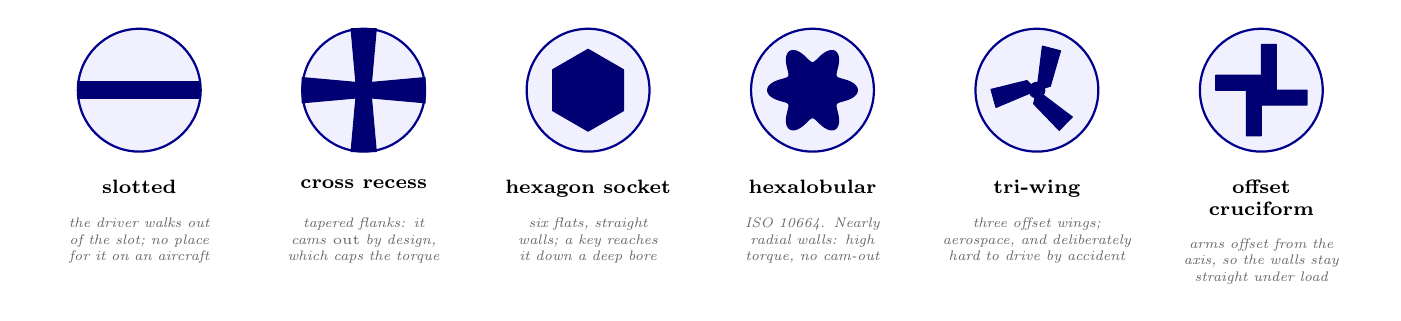
\begin{tikzpicture}[>=Latex,line join=round,line cap=round]
\tikzset{
  headc/.style={fill=blue!6,draw=blue!55!black,thick},
  rec/.style={fill=blue!45!black,draw=blue!45!black},
  lbl/.style={font=\scriptsize\bfseries,align=center,text width=2.6cm,anchor=north},
  sub/.style={font=\tiny\itshape,align=center,text width=2.6cm,text=black!60,anchor=north}
}
\def\R{0.78}

% ---------- 1. slotted ----------
\begin{scope}[xshift=0cm]
\draw[headc] (0,0) circle (\R);
\fill[rec] (-\R,-0.11) rectangle (\R,0.11);
\node[lbl] at (0,-1.02) {slotted};
\node[sub] at (0,-1.50) {the driver walks out of the slot; no place for it on an aircraft};
\end{scope}

% ---------- 2. cross recess (Phillips) ----------
\begin{scope}[xshift=2.85cm]
\draw[headc] (0,0) circle (\R);
\foreach \a in {0,90,180,270}{
  \fill[rec,rotate=\a] (-0.09,0) -- (-0.16,\R) -- (0.16,\R) -- (0.09,0) -- cycle;}
\fill[rec] (0,0) circle (0.11);
\node[lbl] at (0,-1.02) {cross recess};
\node[sub] at (0,-1.50) {tapered flanks: it cams \emph{out} by design, which caps the torque};
\end{scope}

% ---------- 3. hexagon socket ----------
\begin{scope}[xshift=5.70cm]
\draw[headc] (0,0) circle (\R);
\fill[rec] (30:0.52) \foreach \a in {90,150,...,330}{ -- (\a:0.52)} -- cycle;
\node[lbl] at (0,-1.02) {hexagon socket};
\node[sub] at (0,-1.50) {six flats, straight walls; a key reaches it down a deep bore};
\end{scope}

% ---------- 4. hexalobular (ISO 10664) ----------
\begin{scope}[xshift=8.55cm]
\draw[headc] (0,0) circle (\R);
\fill[rec,domain=0:360,samples=240,smooth cycle,variable=\t]
  plot ({(0.46+0.11*cos(6*\t))*cos(\t)},{(0.46+0.11*cos(6*\t))*sin(\t)});
\node[lbl] at (0,-1.02) {hexalobular};
\node[sub] at (0,-1.50) {ISO 10664. Nearly radial walls: high torque, no cam-out};
\end{scope}

% ---------- 5. tri-wing ----------
\begin{scope}[xshift=11.40cm]
\draw[headc] (0,0) circle (\R);
\foreach \a in {0,120,240}{
  \fill[rec,rotate=\a] (0.00,0.00) -- (0.07,0.56) -- (0.30,0.50) -- (0.17,0.05) -- cycle;}
\fill[rec] (0,0) circle (0.10);
\node[lbl] at (0,-1.02) {tri-wing};
\node[sub] at (0,-1.50) {three offset wings; aerospace, and deliberately hard to drive by accident};
\end{scope}

% ---------- 6. offset cruciform (Torq-Set) ----------
\begin{scope}[xshift=14.25cm]
\draw[headc] (0,0) circle (\R);
\foreach \a in {0,90,180,270}{
  \fill[rec,rotate=\a] (0.00,0.06) -- (0.00,0.58) -- (0.19,0.58) -- (0.19,-0.06) -- cycle;}
\fill[rec] (0,0) circle (0.10);
\node[lbl] at (0,-1.02) {offset\\ cruciform};
\node[sub] at (0,-1.76) {arms offset from the axis, so the walls stay straight under load};
\end{scope}

\end{tikzpicture}
}
\vfill
\raggedright
The drive decides the torque you can apply, so it decides the \textbf{preload you can achieve}. The
distinction that matters is \alert{cam-out}.
\vfill
\begin{columns}[T]
\begin{column}{0.48\textwidth}
{\footnotesize
\textbf{Cams out} --- torque-limited by its own shape\\
\emph{slot}: no centring at all; no place on an aircraft\\
\emph{cross recess}: tapered flanks push the driver \emph{out} --- by design. A torque cap is the
last thing you want when preload is the point.}
\end{column}
\begin{column}{0.48\textwidth}
{\footnotesize
\textbf{Does not cam out} --- nearly radial walls\\
\emph{hex socket} (ISO 4762), \emph{hexalobular} (ISO 10664)\\
\emph{tri-wing}, \emph{offset cruciform}: aerospace, and deliberately not driveable by anyone who
happens to own a screwdriver.}
\end{column}
\end{columns}
\end{frame}

\begin{frame}{What has to be on the drawing}
\begin{alertblock}{For every threaded fastener in a structural joint}
\begin{columns}[T]
\begin{column}{0.48\textwidth}
\vspace{4pt}
\begin{itemize}
\item thread designation \textbf{and class}
\item head type --- and if flush, the \textbf{included angle}
\item drive type \textbf{and standard}
\item grip length
\end{itemize}
\end{column}
\begin{column}{0.48\textwidth}
\vspace{4pt}
\begin{itemize}
\item under-head fillet and the matching hole chamfer
\item washer --- \textbf{and which way up}
\item preload or tightening torque, \textbf{and the method}
\item locking method
\end{itemize}
\end{column}
\end{columns}
\end{alertblock}
\vfill
\centering
\large Leave any one of these to the shop floor, and you have delegated a structural decision to
someone who was never told it was one.
\end{frame}

\section{Calling out the fastener}


\section{Nuts, locking and preload}

\begin{frame}{The nut is a designed component}
\centering
\resizebox{0.99\textwidth}{!}{% Nut types and how each one is locked.
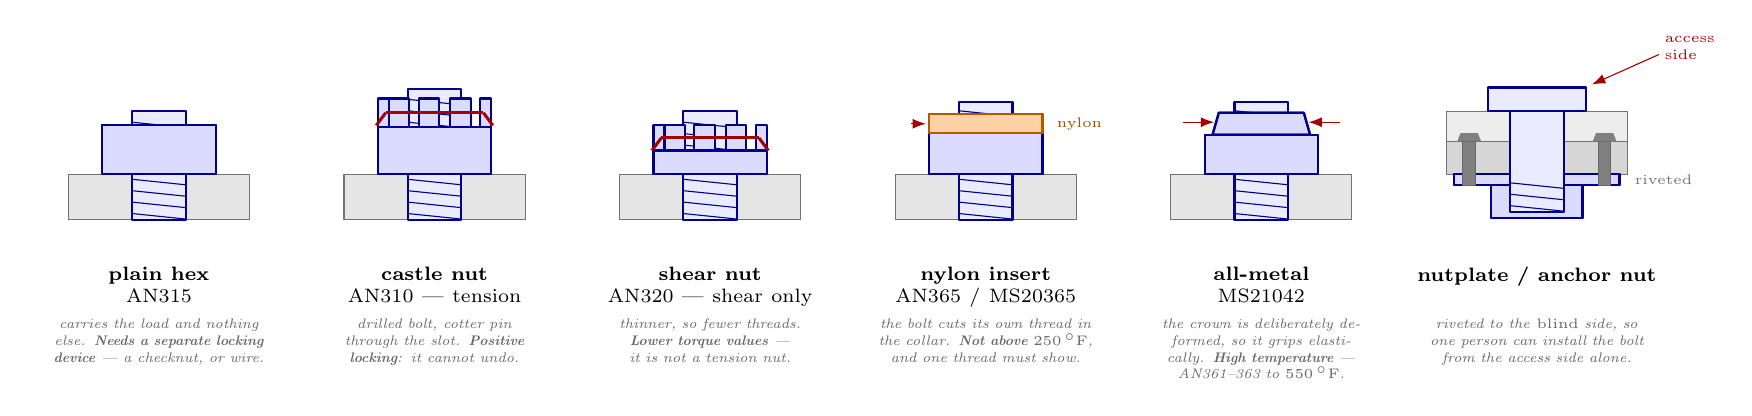
\begin{tikzpicture}[>=Latex,line join=round]
\tikzset{
  steel/.style={fill=blue!8,draw=blue!55!black,thick},
  nutf/.style={fill=blue!14,draw=blue!55!black,thick},
  nylon/.style={fill=orange!35,draw=orange!70!black,thick},
  plate/.style={fill=black!10,draw=black!55},
  pin/.style={draw=red!65!black,line width=1.1pt},
  lbl/.style={font=\scriptsize\bfseries,align=center,text width=3.1cm,anchor=north},
  sub/.style={font=\tiny\itshape,align=center,text width=3.1cm,text=black!60,anchor=north},
  ar/.style={->,red!65!black,thin}
}
% \bolt{x}{top y}
\newcommand{\bolt}[2]{%
  \draw[steel] (#1-0.34,-0.58) rectangle (#1+0.34,#2);
  \foreach \k in {0,1,...,11}{%
    \pgfmathsetmacro\yy{-0.50+0.145*\k}
    \ifdim\yy pt<#2 pt \draw[blue!55!black,thin] (#1-0.34,\yy) -- (#1+0.34,\yy-0.07);\fi}
}
\newcommand{\plat}[1]{\fill[plate] (#1-1.15,-0.58) rectangle (#1+1.15,0);
  \draw[black!55] (#1-1.15,-0.58) -- (#1-0.34,-0.58) (#1+0.34,-0.58) -- (#1+1.15,-0.58);
  \draw[black!55] (#1-1.15,0) -- (#1-0.34,0) (#1+0.34,0) -- (#1+1.15,0);}
% castellations on top of a nut: {x}{base y}{top y}
\newcommand{\castle}[3]{%
  \foreach \c in {-0.58,-0.20,0.20}{
    \fill[nutf] (#1+\c,#2) rectangle (#1+\c+0.26,#3);}
  \fill[nutf] (#1+0.58,#2) rectangle (#1+0.72,#3);
  \fill[nutf] (#1-0.72,#2) rectangle (#1-0.58,#3);}

%============ 1. plain hex ============
\def\x{0}
\plat{\x}\bolt{\x}{0.80}
\fill[nutf] (\x-0.72,0) rectangle (\x+0.72,0.62);
\draw[blue!55!black,thick] (\x-0.72,0) rectangle (\x+0.72,0.62);
\node[lbl] at (\x,-1.05) {plain hex\\ \mdseries AN315};
\node[sub] at (\x,-1.72) {carries the load and nothing else. \textbf{Needs a separate locking device} --- a checknut, or wire.};

%============ 2. castle nut + cotter pin ============
\def\x{3.5}
\plat{\x}\bolt{\x}{1.08}
\fill[nutf] (\x-0.72,0) rectangle (\x+0.72,0.60);
\draw[blue!55!black,thick] (\x-0.72,0) rectangle (\x+0.72,0.60);
\castle{\x}{0.60}{0.96}
\draw[blue!55!black,thick] (\x-0.72,0.60) -- (\x+0.72,0.60);
\draw[pin] (\x-0.62,0.78) -- (\x+0.62,0.78);
\draw[pin] (\x+0.62,0.78) -- (\x+0.74,0.62);
\draw[pin] (\x-0.62,0.78) -- (\x-0.74,0.62);
\node[lbl] at (\x,-1.05) {castle nut\\ \mdseries AN310 --- tension};
\node[sub] at (\x,-1.72) {drilled bolt, cotter pin through the slot. \textbf{Positive locking}: it cannot undo.};

%============ 3. castellated shear nut ============
\def\x{7.0}
\plat{\x}\bolt{\x}{0.80}
\fill[nutf] (\x-0.72,0) rectangle (\x+0.72,0.30);
\draw[blue!55!black,thick] (\x-0.72,0) rectangle (\x+0.72,0.30);
\castle{\x}{0.30}{0.62}
\draw[blue!55!black,thick] (\x-0.72,0.30) -- (\x+0.72,0.30);
\draw[pin] (\x-0.62,0.46) -- (\x+0.62,0.46);
\draw[pin] (\x+0.62,0.46) -- (\x+0.74,0.30);
\draw[pin] (\x-0.62,0.46) -- (\x-0.74,0.30);
\node[lbl] at (\x,-1.05) {shear nut\\ \mdseries AN320 --- shear only};
\node[sub] at (\x,-1.72) {thinner, so fewer threads. \textbf{Lower torque values} --- it is not a tension nut.};

%============ 4. fibre / nylon insert ============
\def\x{10.5}
\plat{\x}\bolt{\x}{0.92}
\fill[nutf] (\x-0.72,0) rectangle (\x+0.72,0.52);
\draw[blue!55!black,thick] (\x-0.72,0) rectangle (\x+0.72,0.52);
\fill[nylon] (\x-0.72,0.52) rectangle (\x+0.72,0.76);
\draw[orange!70!black,thick] (\x-0.72,0.52) rectangle (\x+0.72,0.76);
\node[font=\tiny,text=orange!60!black,anchor=west] at (\x+0.78,0.64) {nylon};
\draw[ar] (\x-0.95,0.64) -- (\x-0.76,0.64);
\node[lbl] at (\x,-1.05) {nylon insert\\ \mdseries AN365 / MS20365};
\node[sub] at (\x,-1.72) {the bolt cuts its own thread in the collar. \textbf{Not above \SI{250}{\degree F}}, and one thread must show.};

%============ 5. all-metal self-locking ============
\def\x{14.0}
\plat{\x}\bolt{\x}{0.92}
\fill[nutf] (\x-0.72,0) rectangle (\x+0.72,0.50);
\draw[blue!55!black,thick] (\x-0.72,0) rectangle (\x+0.72,0.50);
\fill[nutf] (\x-0.62,0.50) -- (\x+0.62,0.50) -- (\x+0.54,0.78) -- (\x-0.54,0.78) -- cycle;
\draw[blue!55!black,thick] (\x-0.62,0.50) -- (\x+0.62,0.50) (\x-0.62,0.50) -- (\x-0.54,0.78)
  -- (\x+0.54,0.78) -- (\x+0.62,0.50);
\draw[ar] (\x-1.00,0.66) -- (\x-0.60,0.66);
\draw[ar] (\x+1.00,0.66) -- (\x+0.60,0.66);
\node[lbl] at (\x,-1.05) {all-metal\\ \mdseries MS21042};
\node[sub] at (\x,-1.72) {the crown is deliberately deformed, so it grips elastically. \textbf{High temperature} ---\\ AN361--363 to \SI{550}{\degree F}.};

%============ 6. nutplate / anchor nut ============
\def\x{17.5}
% the part being attached (light), on the structure (darker)
\fill[black!7,draw=black!55] (\x-1.15,0.42) rectangle (\x+1.15,0.80);
\fill[black!16,draw=black!55] (\x-1.15,0.00) rectangle (\x+1.15,0.42);
% nutplate: body hanging below, flange pressed to the blind face
\fill[nutf] (\x-0.58,-0.56) rectangle (\x+0.58,-0.14);
\draw[blue!55!black,thick] (\x-0.58,-0.56) rectangle (\x+0.58,-0.14);
\fill[nutf] (\x-1.05,-0.14) rectangle (\x+1.05,0.00);
\draw[blue!55!black,thick] (\x-1.05,-0.14) rectangle (\x+1.05,0.00);
% rivets through flange and structure
\foreach \r in {-0.86,0.86}{
  \fill[black!50,draw=black!60] (\x+\r-0.08,-0.14) rectangle (\x+\r+0.08,0.42);
  \fill[black!50] (\x+\r-0.15,0.42) -- (\x+\r+0.15,0.42) -- (\x+\r+0.11,0.52) -- (\x+\r-0.11,0.52) -- cycle;}
% the bolt, installed from the access side
\draw[steel] (\x-0.34,0.80) rectangle (\x+0.34,-0.48);
\foreach \k in {0,1,2}{\draw[blue!55!black,thin] (\x-0.34,-0.40+0.145*\k) -- (\x+0.34,-0.47+0.145*\k);}
\fill[blue!8,draw=blue!55!black,thick] (\x-0.62,0.80) rectangle (\x+0.62,1.10);
% access-side arrow
\draw[ar] (\x+1.55,1.52) -- (\x+0.70,1.14);
\node[font=\tiny,text=red!65!black,anchor=west,align=left] at (\x+1.50,1.60) {access\\ side};
\node[font=\tiny,text=black!55,anchor=west] at (\x+1.12,-0.07) {riveted};
\node[lbl] at (\x,-1.05) {nutplate / anchor nut};
\node[sub] at (\x,-1.72) {riveted to the \emph{blind} side, so one person can install the bolt from the access side alone.};

\end{tikzpicture}
}
\vfill
\raggedright
Only the middle two lock \textbf{positively}. The next two lock by \textbf{friction}. The first does
not lock at all --- and nor, whatever it looks like, does a spring washer.
\end{frame}

\begin{frame}{A shear nut is not a small tension nut}
The castle nut (AN310) and the castellated shear nut (AN320) look alike and thread onto the same
bolt. The FAA torque tables list them \alert{separately}.
\vfill
\begin{columns}[T]
\begin{column}{0.46\textwidth}
\begin{block}{Why}
The shear nut is thinner and has \textbf{fewer engaged threads}. AN320 is ``designed for use with
hardware subjected to shear stress only''.
\end{block}
\end{column}
\begin{column}{0.50\textwidth}
\begin{alertblock}{What goes wrong}
Thread engagement decides whether the \textbf{bolt breaks} or the \textbf{thread strips}.
\vspace{2pt}
Put a shear nut on a bolt in tension and you have moved the weak link from the bolt --- where you
designed it to be --- to the thread, where you did not.
\end{alertblock}
\end{column}
\end{columns}
\end{frame}

\begin{frame}{Locking is positive, or it is not locking}
Three things, and only three, are accepted.
\vfill
\begin{columns}[T]
\begin{column}{0.32\textwidth}
\begin{block}{1. Cotter pin}
through a castellated nut. The nut physically \textbf{cannot} rotate.
\vspace{2pt}
{\scriptsize Costs a drilled bolt, and the slot must align \emph{inside} the torque band. If it
will not: change the washer or the nut --- never the torque.}
\end{block}
\end{column}
\begin{column}{0.32\textwidth}
\begin{block}{2. Safety wire}
A tension member --- and tension has a \textbf{sign}.
\vspace{2pt}
{\scriptsize The one most often installed backwards. See the next slide.}
\end{block}
\end{column}
\begin{column}{0.32\textwidth}
\begin{block}{3. Self-locking nut}
with a \textbf{specified prevailing torque}.
\vspace{2pt}
{\scriptsize Friction --- accepted only because the friction is a measured, specified quantity.}
\end{block}
\end{column}
\end{columns}
\vfill
\centering
Neither cotter pins nor safety wire are ever reused.
\end{frame}

\begin{frame}{The safety-wire direction rule}
\centering
\resizebox{!}{3.6cm}{% Safety wire: the direction rule. Bolt heads in plan, right-hand threads.
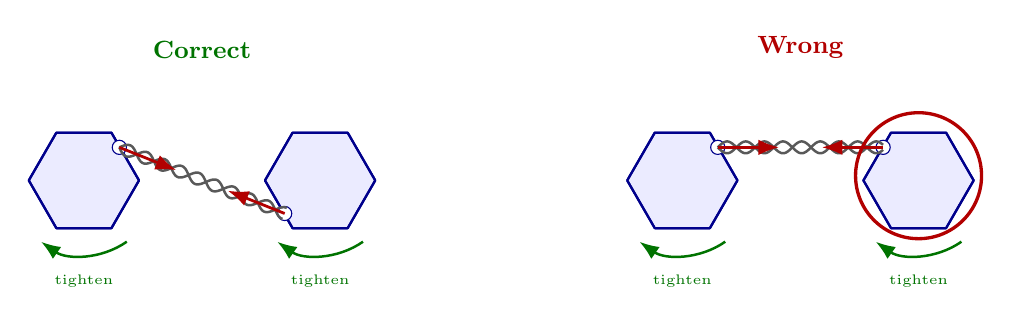
\begin{tikzpicture}[>=Latex,line join=round]
\tikzset{
  hd/.style={fill=blue!8,draw=blue!55!black,thick},
  hole/.style={fill=white,draw=blue!55!black,thin},
  wire/.style={draw=black!65,line width=0.9pt},
  tens/.style={->,red!70!black,line width=1.0pt},
  spin/.style={->,green!45!black,line width=0.9pt},
  ok/.style={font=\small\bfseries,text=green!45!black},
  no/.style={font=\small\bfseries,text=red!70!black},
  cp/.style={font=\scriptsize,align=center,text width=6.4cm,anchor=north}
}
% hex head in plan at (#1,#2)
\newcommand{\head}[2]{%
  \fill[hd] (#1,#2) +(0:0.70) \foreach \a in {60,120,...,300}{ -- +(\a:0.70)} -- cycle;
  \draw[blue!55!black,thick] (#1,#2) +(0:0.70) \foreach \a in {60,120,...,300}{ -- +(\a:0.70)} -- cycle;
  \draw[spin] ([shift=(305:0.95)]#1,#2) arc (305:235:0.95);
  \node[font=\tiny,text=green!45!black,anchor=north] at (#1,#2-1.08) {tighten};}
% twisted wire from (#1,#2) to (#3,#4)
\newcommand{\twist}[4]{%
  \pgfmathsetmacro\dxx{#3-#1}\pgfmathsetmacro\dyy{#4-#2}
  \pgfmathsetmacro\len{sqrt(\dxx*\dxx+\dyy*\dyy)}
  \pgfmathsetmacro\rot{atan2(\dyy,\dxx)}
  \begin{scope}[shift={(#1,#2)},rotate=\rot]
    \draw[wire,domain=0:\len,samples=160,variable=\t] plot ({\t},{ 0.075*sin(760*\t)});
    \draw[wire,domain=0:\len,samples=160,variable=\t] plot ({\t},{-0.075*sin(760*\t)});
  \end{scope}}

%=================== (a) correct ===================
\begin{scope}
\head{0}{0}\head{3.0}{0}
\fill[hole] (0.45,0.42) circle (0.09);
\fill[hole] (2.55,-0.42) circle (0.09);
\twist{0.45}{0.42}{2.55}{-0.42}
% tension at each hole, in the tightening sense
\draw[tens] (0.45,0.42) -- ++(-21.8:0.78);
\draw[tens] (2.55,-0.42) -- ++(158.2:0.78);
\node[ok,anchor=south] at (1.5,1.42) {Correct};
\end{scope}

%=================== (b) wrong ===================
\begin{scope}[xshift=7.6cm]
\head{0}{0}\head{3.0}{0}
\fill[hole] (0.45,0.42) circle (0.09);
\fill[hole] (2.55,0.42) circle (0.09);
\twist{0.45}{0.42}{2.55}{0.42}
\draw[tens] (0.45,0.42) -- ++(0:0.78);
\draw[tens] (2.55,0.42) -- ++(180:0.78);
\draw[red!70!black,very thick] (3.0,0.06) circle (0.80);
\node[no,anchor=south] at (1.5,1.42) {Wrong};
\end{scope}

\end{tikzpicture}
}
\vfill
\raggedright
AC 43.13-1B \S7-127: ``\emph{wire should always be applied so that tension is in the tightening
direction}''.
\vfill
{\footnotesize \SI{0.032}{in} minimum wire for holes over \SI{0.045}{in} \ $\cdot$ \ pulled taut
when twisting, but left under \emph{light} tension --- ``safety wire will break under vibrations if
twisted too tightly'' \ $\cdot$ \ four to six turns after the loop \ $\cdot$ \ ends bent under and
inward.}
\end{frame}

\begin{frame}{A rule everyone quotes that is not in the regulation}
\begin{alertblock}{You will hear this}
``No more than \textbf{three} fasteners wired in a group, and never more than \textbf{24 inches}
of wire.''
\end{alertblock}
\vfill
It is not in AC 43.13-1B. What \S7-124a actually says is that closely grouped parts may be wired in
series, and that
\vfill
\begin{block}{}
\centering\large
``\emph{the number of bolts, nuts, screws, etc., that may be wired together depends on the
application.}''
\end{block}
\vfill
\centering
A number repeated confidently in a hangar, in a forum, and in a set of lecture notes is still not a
requirement. \alert{When it matters, read the document.}
\end{frame}

\begin{frame}{Prevailing torque is a specification, not a feeling}
\textbf{Run-on torque} is the torque to turn the nut \emph{before it seats} --- before any preload
exists. It has a minimum \alert{and} a maximum.
\vfill
\begin{columns}[T]
\begin{column}{0.48\textwidth}
\begin{block}{Too low}
The nut is not locking. ``DO NOT reuse a fiber or nylon locknut if the nut cannot meet the minimum
prevailing torque values'' --- which are tabulated.
\end{block}
\end{column}
\begin{column}{0.48\textwidth}
\begin{block}{Too high}
It eats the torque budget: the wrench reading now contains a term that never becomes preload.
\vspace{2pt}
Specify \textbf{torque $+$ measured run-on drag}.
\end{block}
\end{column}
\end{columns}
\vfill
\begin{alertblock}{And what it may not do --- AC 43.13-1B \S7-64, Table 7-13}
{\footnotesize
\textbf{``DO NOT use self-locking nuts on parts subject to rotation.''} \ $\cdot$ \ nylon not above
\SI{250}{\degree F}; all-metal AN361--363 to \SI{550}{\degree F} \ $\cdot$ \ not where a loose item
could reach a turbine intake \ $\cdot$ \ not on panels routinely removed \ $\cdot$ \ \textbf{at
least one thread must show past the nut}.}
\end{alertblock}
\end{frame}

\begin{frame}{So what do you use instead of a torque wrench?}
\centering
\resizebox{!}{4.5cm}{% What preload you actually get, by method. Data: IFI, via NASA RP-1228 Table VII.
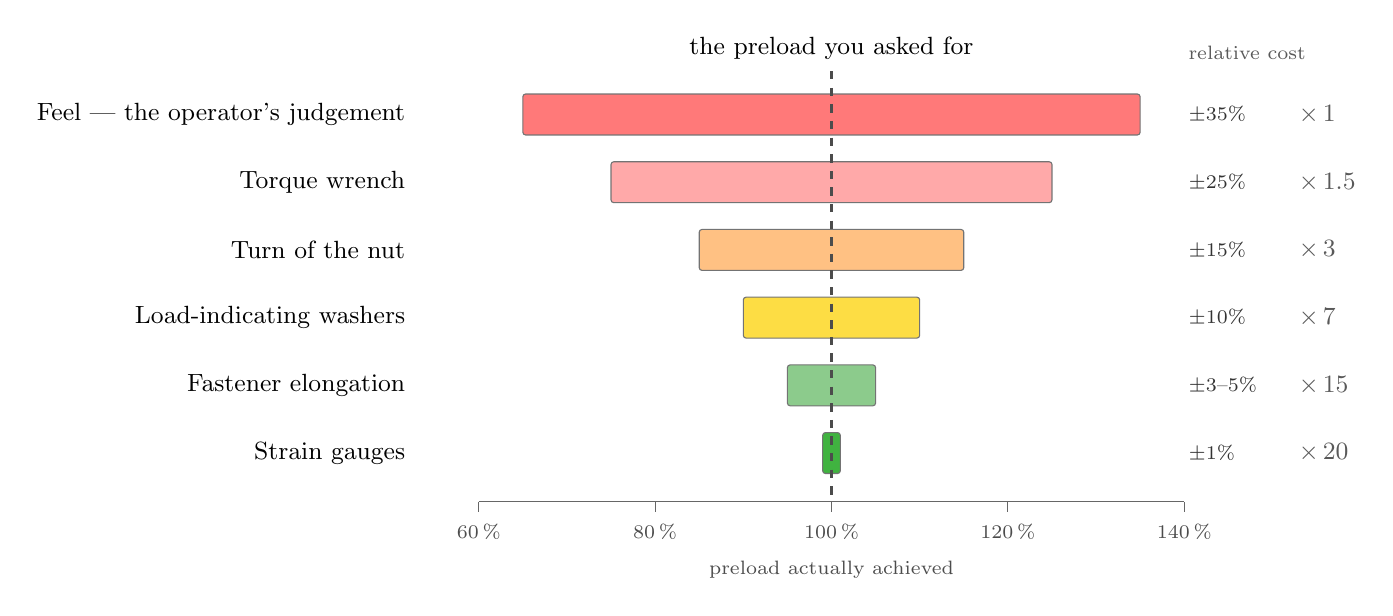
\begin{tikzpicture}[>=Latex]
\tikzset{
  nm/.style={font=\small,anchor=east},
  ct/.style={font=\small,anchor=west,text=black!65},
  ax/.style={font=\scriptsize,text=black!70}
}
\def\X#1{(#1-55)*0.112}          % percent -> cm
\def\dy{0.86}

% ---- band for each method ----
% {row}{name}{tolerance}{cost}{colour}
\foreach \i/\nmm/\tol/\cost/\col in {
  0/{Feel --- the operator's judgement}/35/1/{red!70},
  1/{Torque wrench}/25/{1.5}/{red!45},
  2/{Turn of the nut}/15/3/{orange!65},
  3/{Load-indicating washers}/10/7/{yellow!70!orange},
  4/{Fastener elongation}/5/15/{green!55!black!60},
  5/{Strain gauges}/1/20/{green!60!black}}
{
  \pgfmathsetmacro\y{-\i*\dy}
  \fill[\col,opacity=0.75,rounded corners=1pt]
    ({\X{100-\tol}},\y-0.26) rectangle ({\X{100+\tol}},\y+0.26);
  \draw[black!55,thin,rounded corners=1pt]
    ({\X{100-\tol}},\y-0.26) rectangle ({\X{100+\tol}},\y+0.26);
  \node[nm] at (-0.25,\y) {\nmm};
  \node[ct] at (10.85,\y) {$\times\,\cost$};
}
% explicit tolerance labels (elongation is a range)
\foreach \i/\txt in {0/{$\pm35\%$},1/{$\pm25\%$},2/{$\pm15\%$},3/{$\pm10\%$},
                     4/{$\pm3$--$5\%$},5/{$\pm1\%$}}{
  \pgfmathsetmacro\y{-\i*\dy}
  \node[font=\scriptsize,anchor=west,text=black!80] at (9.45,\y) {\txt};
}

% ---- target line and axis ----
\draw[black!70,thick,dashed] ({\X{100}},0.55) -- ({\X{100}},-5*\dy-0.55);
\node[font=\small,anchor=south] at ({\X{100}},0.58) {the preload you asked for};

\draw[black!60] ({\X{60}},-5*\dy-0.62) -- ({\X{140}},-5*\dy-0.62);
\foreach \p in {60,80,100,120,140}{
  \draw[black!60] ({\X{\p}},-5*\dy-0.62) -- ({\X{\p}},-5*\dy-0.75);
  \node[ax,anchor=north] at ({\X{\p}},-5*\dy-0.78) {\p\,\%};}
\node[ax,anchor=north] at ({\X{100}},-5*\dy-1.25) {preload actually achieved};
\node[font=\scriptsize,anchor=south west,text=black!65] at (9.45,0.58) {relative cost};

\end{tikzpicture}
}
\vfill
\raggedright
{\footnotesize Industrial Fasteners Institute, via NASA RP-1228.} Accuracy costs money in a fixed
ratio. The question is never ``which is best'' but ``\emph{how much scatter can this joint
absorb}''.
\end{frame}

\begin{frame}{Turn of the nut --- and why it is a long-bolt method}
Turning the nut by $\theta$ advances it $(\theta/360)p$ along the thread, and that take-up is shared
between bolt stretch and member squash. \alert{No friction appears anywhere in it.}
\[
\frac{\theta}{360}\,p = F_i\!\left(\frac{1}{k_b}+\frac{1}{k_m}\right)
\qquad\Longrightarrow\qquad
\theta = \frac{360\,F_i}{p}\left(\frac{1}{k_b}+\frac{1}{k_m}\right)
\]
\vfill
\begin{columns}[T]
\begin{column}{0.48\textwidth}
\begin{block}{The M10 joint, \SI{30}{mm} grip}
$\theta = \SI{22.3}{\degree}$ --- a sixteenth of a turn.
\vspace{2pt}
$\pm\SI{5}{\degree}$, which is nothing by hand, is \alert{$\pm\SI{22}{\percent}$ preload} --- no
better than the wrench we just rejected.
\end{block}
\end{column}
\begin{column}{0.48\textwidth}
\begin{block}{Same bolt, \SI{100}{mm} grip}
$\theta = \SI{74.5}{\degree}$.
\vspace{2pt}
The same $\pm\SI{5}{\degree}$ is now $\pm\SI{7}{\percent}$.
\end{block}
\end{column}
\end{columns}
\vfill
\centering
Which is why structural steelwork specifies thirds of a turn, and aerospace usually does not.
\end{frame}

\begin{frame}{Two things no method will do for you}
\begin{alertblock}{Elastic interaction}
Tightening one bolt \textbf{relaxes its neighbours} --- the member compression it creates locally
unloads the bolts already done.
\vspace{2pt}
So: cross pattern, several passes, first pass deliberately low. One perfect pass, bolt by bolt,
gives a ring of unequal preloads.
\end{alertblock}
\vfill
\begin{alertblock}{Embedment and relaxation}
Asperities under the head, under the nut and at every interface yield in the first hours and
\textbf{lose preload} --- a few per cent, more with soft members, coatings or many interfaces.
\vspace{2pt}
Hence the re-torque interval --- and the washer earns its place twice: once for stiffness, once for
bearing.
\end{alertblock}
\end{frame}

\begin{frame}{A preload is not specified until the drawing says}
\begin{columns}[T]
\begin{column}{0.48\textwidth}
\begin{block}{1 --- the number}
the target preload, or the torque \textbf{and the $K$ it was derived from}
\end{block}
\begin{block}{2 --- the method}
and its tolerance
\end{block}
\end{column}
\begin{column}{0.48\textwidth}
\begin{block}{3 --- the condition}
the lubrication and plating the number assumes
\end{block}
\begin{block}{4 --- the lock}
including prevailing-torque limits, if it is a self-locking nut
\end{block}
\end{column}
\end{columns}
\vfill
\centering
\large A torque figure on its own is a number without a meaning.
\end{frame}

\begin{frame}{Calling out a fastener}
\centering\small
\begin{tabular}{@{}ll@{}}
\toprule
\textbf{AN} & Air Force--Navy; oldest family, still common in general aviation\\
\textbf{MS} & Military Standard; largely superseded by NASM\\
\textbf{NAS} & National Aerospace Standard; higher strength, close tolerance\\
\textbf{NASM} & NAS + MS merged; current designation for many former MS items\\
\textbf{EN / LN} & European and German equivalents\\
\bottomrule
\end{tabular}
\vfill
\raggedright
Two habits that will keep you out of trouble:
\begin{itemize}
  \item never substitute a part number you have not looked up;
  \item never assume a dash number means the same thing in two families.
\end{itemize}
\vfill
\begin{alertblock}{Grip length}
The \textbf{grip} is the unthreaded shank. Specify it so the thread run-out is clear of the shear
plane --- otherwise the joint bears on \emph{threads}: a reduced, notched section. The bolt looks
right and torques up correctly. More in Lecture 6.
\end{alertblock}
\end{frame}

\begin{frame}{Decoding a part number --- and its limits}
\centering
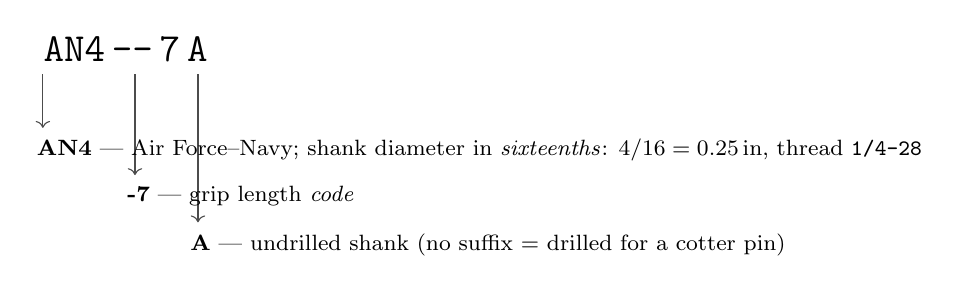
\begin{tikzpicture}[font=\small]
\node (p) at (0,0) {\Large\texttt{AN4\,--\,7\,A}};
\draw[->,gray!60!black] (-1.05,-0.32) -- (-1.05,-1.0);
\draw[->,gray!60!black] (0.12,-0.32) -- (0.12,-1.6);
\draw[->,gray!60!black] (0.92,-0.32) -- (0.92,-2.2);
\node[anchor=north west,align=left,font=\footnotesize] at (-1.25,-1.02)
  {\textbf{AN4} --- Air Force--Navy; shank diameter in \emph{sixteenths}: $4/16=\SI{0.25}{in}$,
   thread \texttt{1/4-28}};
\node[anchor=north west,align=left,font=\footnotesize] at (-0.1,-1.62)
  {\textbf{-7} --- grip length \emph{code}};
\node[anchor=north west,align=left,font=\footnotesize] at (0.7,-2.22)
  {\textbf{A} --- undrilled shank (no suffix $=$ drilled for a cotter pin)};
\end{tikzpicture}
\vfill
\raggedright
\begin{alertblock}{The part you must not infer}
The dash-to-grip conversion is \emph{not} the same across series. Read it from the controlling
standard's table --- never from the pattern you think you spotted in another family.\\[4pt]
\alert{A part number is a lookup, not a language you can speak fluently.}
\end{alertblock}
\end{frame}

\begin{frame}{Construction: thread run-out and relief}
\centering
\resizebox{0.95\textwidth}{!}{
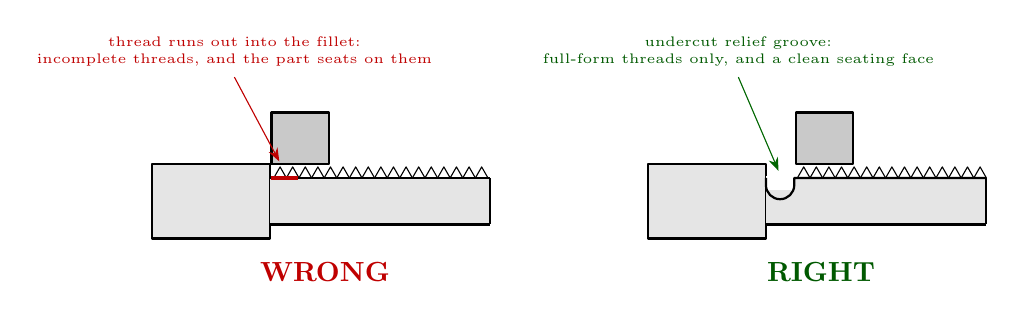
\begin{tikzpicture}[scale=1.0,>=Stealth,font=\scriptsize,line join=round]
\tikzset{bod/.style={thick,fill=gray!20},prt/.style={thick,fill=gray!42}}
\def\thr#1#2#3{\foreach \i in {0,...,#3}{\draw[line width=0.4pt] (#1+\i*0.16,#2) -- (#1+\i*0.16+0.08,#2+0.14) -- (#1+\i*0.16+0.16,#2);}}
% ---------------- WRONG ----------------
\begin{scope}
\fill[gray!20] (0,0) rectangle (1.5,0.95); \draw[thick] (0,0) rectangle (1.5,0.95);
\fill[gray!20] (1.5,0.18) rectangle (4.3,0.77); \draw[thick] (1.5,0.18) -- (4.3,0.18);
\draw[thick] (1.5,0.77) -- (4.3,0.77); \draw[thick] (4.3,0.18) -- (4.3,0.77);
\thr{1.55}{0.77}{16}
\draw[red!75!black,line width=1.2pt] (1.50,0.18) arc (270:360:0.0);
\draw[red!75!black,line width=1.3pt] (1.52,0.77) -- (1.52+0.34,0.77);
\draw[prt] (1.52,0.95) rectangle (2.25,1.60);
\draw[->,red!75!black] (1.05,2.05) -- (1.62,0.98);
\node[red!75!black,anchor=south,align=center,font=\tiny] at (1.05,2.07)
  {thread runs out into the fillet:\\ incomplete threads, and the part
   seats on them};
\node[anchor=north,font=\bfseries,red!75!black] at (2.2,-0.18) {WRONG};
\end{scope}
% ---------------- RIGHT ----------------
\begin{scope}[xshift=6.3cm]
\fill[gray!20] (0,0) rectangle (1.5,0.95); \draw[thick] (0,0) rectangle (1.5,0.95);
\fill[gray!20] (1.5,0.18) rectangle (4.3,0.77);
\draw[thick] (1.5,0.18) -- (4.3,0.18);
\draw[thick] (4.3,0.18) -- (4.3,0.77);
% undercut relief groove
\fill[white] (1.50,0.62) rectangle (1.86,0.80);
\draw[thick] (1.50,0.77) -- (1.50,0.68) arc (180:360:0.18) -- (1.86,0.77) -- (4.3,0.77);
\thr{1.90}{0.77}{14}
\draw[->,green!40!black] (1.15,2.05) -- (1.66,0.86);
\node[green!35!black,anchor=south,align=center,font=\tiny] at (1.15,2.07)
  {undercut relief groove:\\ full-form threads only, and a
   clean seating face};
\draw[prt] (1.88,0.95) rectangle (2.61,1.60);
\node[anchor=north,font=\bfseries,green!35!black] at (2.2,-0.18) {RIGHT};
\end{scope}
\end{tikzpicture}
}
\vfill
\raggedright
The last turn or two of any cut or rolled thread is \textbf{incomplete} --- it cannot carry full load
and it cannot seat a part squarely. Run it into a fillet and you have put a stress concentration and a
bad seating face in the same place.
\vfill
{\small The relief groove costs one operation and a little section. It buys a full-form thread
everywhere it is used, and a face the mating part can sit on.}
\end{frame}

\begin{frame}{Construction: get the grip length right}
\centering
\resizebox{0.95\textwidth}{!}{
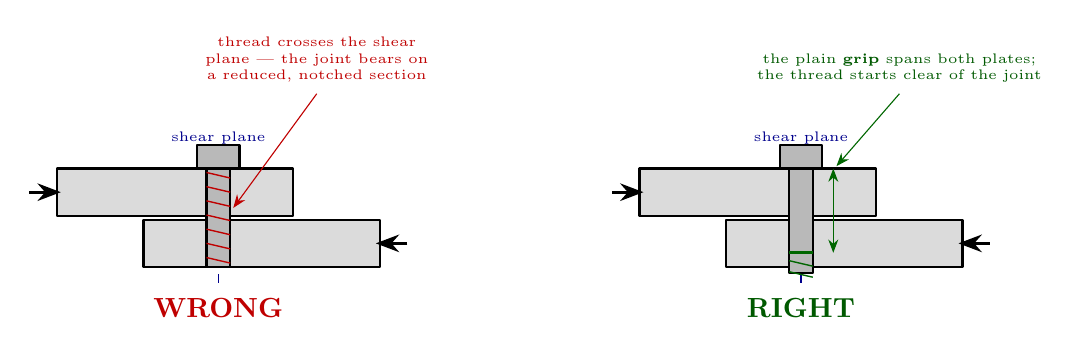
\begin{tikzpicture}[scale=1.0,>=Stealth,font=\scriptsize,line join=round]
\tikzset{pl/.style={thick,fill=gray!28},bl/.style={thick,fill=gray!55}}
% ---------------- WRONG ----------------
\begin{scope}
\draw[pl] (0,1.15) rectangle (3.0,1.75);
\draw[pl] (1.1,0.50) rectangle (4.1,1.10);
\draw[->,very thick] (-0.35,1.45) -- (0.05,1.45);
\draw[->,very thick] (4.45,0.80) -- (4.05,0.80);
\draw[blue!55!black,dashed] (2.05,0.30) -- (2.05,1.92);
\node[blue!55!black,anchor=south,font=\tiny] at (2.05,1.93) {shear plane};
\draw[bl] (1.78,1.75) rectangle (2.32,2.05);
\draw[bl] (1.90,0.50) rectangle (2.20,1.75);
\foreach \y in {0.62,0.80,0.98,1.16,1.34,1.52,1.70}{
  \draw[red!75!black,line width=0.5pt] (1.90,\y) -- (2.20,\y-0.07);}
\draw[->,red!75!black] (3.30,2.70) -- (2.24,1.25);
\node[red!75!black,anchor=south,align=center,font=\tiny,text width=3.6cm] at (3.30,2.72)
  {thread crosses the shear plane --- the joint bears on a reduced, notched section};
\node[anchor=north,font=\bfseries,red!75!black] at (2.05,0.22) {WRONG};
\end{scope}
% ---------------- RIGHT ----------------
\begin{scope}[xshift=7.4cm]
\draw[pl] (0,1.15) rectangle (3.0,1.75);
\draw[pl] (1.1,0.50) rectangle (4.1,1.10);
\draw[->,very thick] (-0.35,1.45) -- (0.05,1.45);
\draw[->,very thick] (4.45,0.80) -- (4.05,0.80);
\draw[blue!55!black,dashed] (2.05,0.30) -- (2.05,1.92);
\node[blue!55!black,anchor=south,font=\tiny] at (2.05,1.93) {shear plane};
\draw[bl] (1.78,1.75) rectangle (2.32,2.05);
\draw[bl] (1.90,0.42) rectangle (2.20,1.75);
\foreach \y in {0.44,0.58}{
  \draw[green!40!black,line width=0.5pt] (1.90,\y) -- (2.20,\y-0.07);}
\draw[green!40!black,line width=1.1pt] (1.90,0.68) -- (2.20,0.68);
\draw[<->,green!40!black] (2.46,0.68) -- (2.46,1.75);

\draw[->,green!40!black] (3.30,2.70) -- (2.50,1.78);
\node[green!35!black,anchor=south,align=center,font=\tiny,text width=3.8cm] at (3.30,2.72)
  {the plain \textbf{grip} spans both plates; the thread starts clear of the joint};
\node[anchor=north,font=\bfseries,green!35!black] at (2.05,0.22) {RIGHT};
\end{scope}
\end{tikzpicture}
}
\vfill
\raggedright
This is the error that hides best: right diameter, right material, right part number, torques up
correctly, looks finished.
\vfill
\begin{alertblock}{And it is bearing on threads}
A reduced diameter, a notched surface and uneven contact --- in \emph{shear}, where a thread is at
its worst. Specify the grip so the run-out clears the joint, and take up the difference with a
washer, not with the thread.
\end{alertblock}
\end{frame}

\begin{frame}{Construction: blind holes, engagement and lead-in}
\centering
\resizebox{0.92\textwidth}{!}{
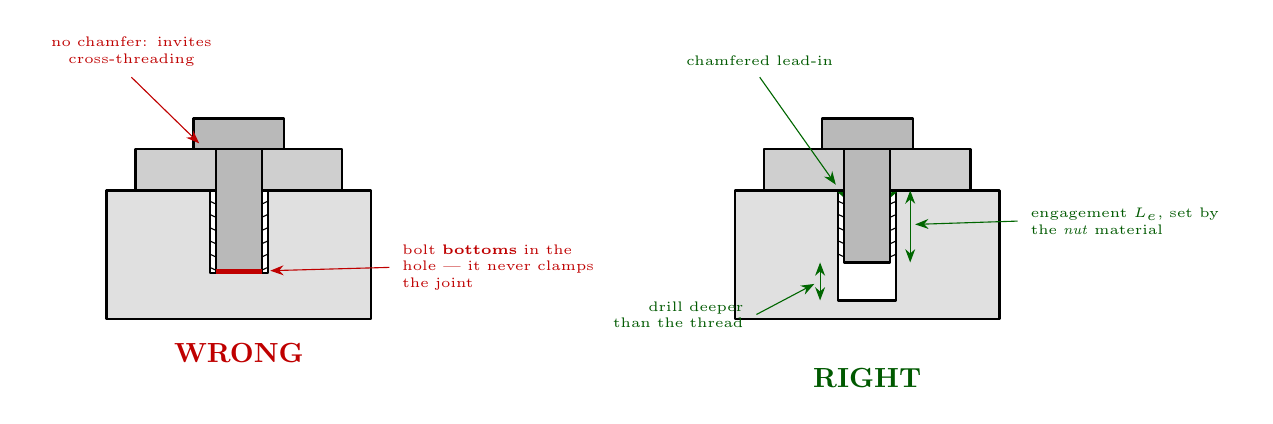
\begin{tikzpicture}[scale=1.05,>=Stealth,font=\scriptsize,line join=round]
\tikzset{bl/.style={thick,fill=gray!55},pl/.style={thick,fill=gray!38}}
% ---------------- WRONG ----------------
\begin{scope}
\fill[gray!24] (0,0) rectangle (3.2,1.55); \draw[thick] (0,0) rectangle (3.2,1.55);
\fill[white] (1.25,0.55) rectangle (1.95,1.55);
\draw[thick] (1.25,1.55) -- (1.25,0.55) -- (1.95,0.55) -- (1.95,1.55);
\foreach \y in {0.62,0.78,0.94,1.10,1.26,1.42}{
  \draw[line width=0.4pt] (1.25,\y) -- (1.40,\y-0.07);
  \draw[line width=0.4pt] (1.95,\y) -- (1.80,\y-0.07);}
\draw[pl] (0.35,1.55) rectangle (2.85,2.05);
\draw[bl] (1.32,0.57) rectangle (1.88,2.05);
\draw[bl] (1.05,2.05) rectangle (2.15,2.42);
\draw[red!75!black,line width=1.5pt] (1.32,0.57) -- (1.88,0.57);
\draw[->,red!75!black] (3.42,0.62) -- (1.98,0.58);
\node[red!75!black,anchor=west,align=left,font=\tiny,text width=2.5cm] at (3.46,0.62)
  {bolt \textbf{bottoms} in the hole --- it never clamps the joint};
\draw[->,red!75!black] (0.30,2.92) -- (1.12,2.12);
\node[red!75!black,anchor=south,align=center,font=\tiny,text width=2.4cm] at (0.30,2.94)
  {no chamfer: invites cross-threading};
\node[anchor=north,font=\bfseries,red!75!black] at (1.6,-0.18) {WRONG};
\end{scope}
% ---------------- RIGHT ----------------
\begin{scope}[xshift=7.6cm]
\fill[gray!24] (0,0) rectangle (3.2,1.55); \draw[thick] (0,0) rectangle (3.2,1.55);
\fill[white] (1.25,0.22) rectangle (1.95,1.55);
\draw[thick] (1.25,1.55) -- (1.25,0.22) -- (1.95,0.22) -- (1.95,1.55);
\foreach \y in {0.78,0.94,1.10,1.26,1.42}{
  \draw[line width=0.4pt] (1.25,\y) -- (1.40,\y-0.07);
  \draw[line width=0.4pt] (1.95,\y) -- (1.80,\y-0.07);}
\draw[green!40!black,line width=1.2pt] (1.25,1.55) -- (1.40,1.42);
\draw[green!40!black,line width=1.2pt] (1.95,1.55) -- (1.80,1.42);
\draw[pl] (0.35,1.55) rectangle (2.85,2.05);
\draw[bl] (1.32,0.68) rectangle (1.88,2.05);
\draw[bl] (1.05,2.05) rectangle (2.15,2.42);
\draw[<->,green!40!black] (2.12,0.68) -- (2.12,1.55);
\draw[->,green!40!black] (3.42,1.18) -- (2.18,1.14);
\node[green!35!black,anchor=west,align=left,font=\tiny,text width=2.6cm] at (3.46,1.18)
  {engagement $L_e$, set by the \emph{nut} material};
\draw[<->,green!40!black] (1.03,0.22) -- (1.03,0.68);
\draw[->,green!40!black] (0.26,0.05) -- (0.96,0.42);
\node[green!35!black,anchor=east,align=right,font=\tiny,text width=2.1cm] at (0.22,0.05)
  {drill deeper than the thread};
\draw[->,green!40!black] (0.30,2.92) -- (1.22,1.62);
\node[green!35!black,anchor=south,align=center,font=\tiny] at (0.30,2.94) {chamfered lead-in};
\node[anchor=north,font=\bfseries,green!35!black] at (1.6,-0.48) {RIGHT};
\end{scope}
\node[anchor=north,font=\bfseries,red!75!black] at (1.6,-0.48) {};
\end{tikzpicture}
}
\vfill
\raggedright
\begin{itemize}
  \item Drill \emph{deeper} than the thread. A bolt that bottoms generates torque without generating
        preload --- the joint reads as tight and is carrying nothing.
  \item Set $L_e$ by the \textbf{nut} material, not by the bolt.
  \item Chamfer the hole mouth. The lead-in is what stops cross-threading, and cross-threading in a
        casting is usually unrecoverable.
\end{itemize}
\end{frame}

\begin{frame}{A bolt circle --- what actually sizes the bolts?}
\begin{center}\small
$D_s=\SI{250}{mm}$ \quad $p=\SI{0.60}{MPa}$ \quad $D_{bc}=\SI{300}{mm}$ \quad grip $l=\SI{20}{mm}$
\end{center}
\vspace{-4pt}
\begin{columns}[T]
\begin{column}{0.47\textwidth}
\begin{block}{\small (a) separating load}
\small
\[ F = p\,\frac{\pi D_s^2}{4} = \SI{29.5}{kN} \]
\end{block}
\begin{block}{\small (b) number of bolts --- from \emph{spacing}}
\small
A sealed flange must stay closed \emph{between} bolts: $s\le 5d$.\\[2pt]
M8: $N \ge \pi(300)/40 = 23.6$\\[2pt]
\centering $\Rightarrow\ \mathbf{N=24}, \ s=\SI{39.3}{mm}=4.9\,d$
\end{block}
\end{column}
\begin{column}{0.49\textwidth}
\begin{block}{\small (c)--(f) the rest falls out}
\small
load per bolt \ $P = 29.5/24 = \SI{1.23}{kN}$\\[3pt]
M8 class 10.9: $F_p=\SI{30.4}{kN}$, $F_i=0.75F_p=\mathbf{\SI{22.8}{kN}}$\\[3pt]
with a washer $C=0.131$, so the bolt rises by\\
$CP=\SI{161}{N}$: \ $22.78 \to \SI{22.94}{kN}$\\[3pt]
$T = K d F_i = \SI{36.5}{N.m}$ dry
\end{block}
\end{column}
\end{columns}
\vspace{2pt}
\centering\alert{\small The separating load adds \SI{161}{N} to a bolt preloaded to \SI{22.8}{kN}.}
\end{frame}

\begin{frame}{Now check the stress cones}
\centering
\resizebox{!}{3.2cm}{
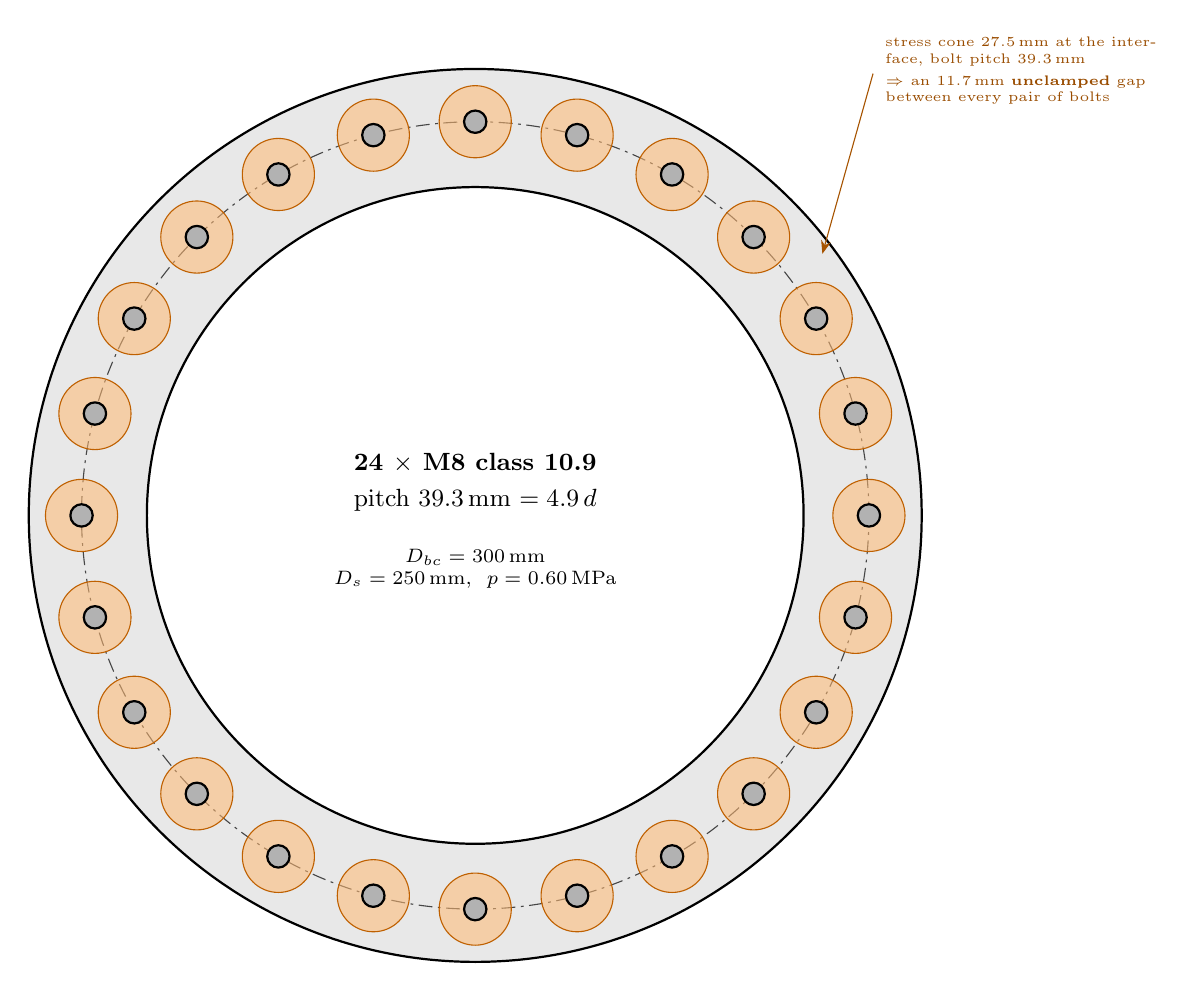
\begin{tikzpicture}[scale=1.0,>=Stealth,font=\scriptsize,line join=round]
% 1 unit = 30 mm.  OD 340, bolt circle 300, bore 250, cone 27.5, hole 8.5
\def\Ro{5.67}\def\Rb{5.00}\def\Ri{4.17}\def\Rc{0.458}\def\Rh{0.142}
\fill[gray!18] (0,0) circle (\Ro);
\fill[white] (0,0) circle (\Ri);
\draw[thick] (0,0) circle (\Ro);
\draw[thick] (0,0) circle (\Ri);
\draw[gray!55!black,dash pattern=on 5pt off 2pt on 1pt off 2pt] (0,0) circle (\Rb);
\foreach \k in {0,...,23}{
  \fill[orange!55,fill opacity=0.55] (\k*15:\Rb) circle (\Rc);
  \draw[orange!75!black,line width=0.4pt] (\k*15:\Rb) circle (\Rc);}
\foreach \k in {0,...,23}{\draw[thick,fill=gray!60] (\k*15:\Rb) circle (\Rh);}
% labels placed in the empty bore
\node[align=center,font=\small] at (0,0.42)
  {\textbf{24 $\times$ M8 class 10.9}\\[2pt] pitch \SI{39.3}{mm} $=4.9\,d$};
\node[anchor=north,align=center,font=\scriptsize] at (0,-0.30)
  {$D_{bc}=\SI{300}{mm}$\\ $D_s=\SI{250}{mm}$, \ $p=\SI{0.60}{MPa}$};
% cone callout
\draw[->,orange!65!black] (48:7.55) -- (37:5.52);
\node[orange!60!black,anchor=west,align=left,font=\tiny,text width=3.5cm] at (48:7.6)
  {stress cone \SI{27.5}{mm} at the interface, bolt pitch \SI{39.3}{mm}\\[2pt]
   $\Rightarrow$ an \SI{11.7}{mm} \textbf{unclamped} gap between every pair of bolts};
\end{tikzpicture}
}
\vfill
\raggedright
{\small At the interface each cone has grown to $16+11.5=\SI{27.5}{mm}$, against a pitch of
\SI{39.3}{mm}. \alert{The cones do not meet.}}
\vspace{3pt}
\begin{alertblock}{Three honest options}
Add bolts (35 at this grip) $\cdot$ thicken the flange so the cones spread further ($l=\SI{40}{mm}$
closes it) $\cdot$ or accept the gap and make the \textbf{flange stiff in bending}.\\[3pt]
Real flanges are thick for exactly this reason: \alert{the driver is flange bending, not bolt
strength.}
\end{alertblock}
\end{frame}

\section{Power screws}

\begin{frame}{Thread forms for power transmission}
\centering
\resizebox{0.98\textwidth}{!}{
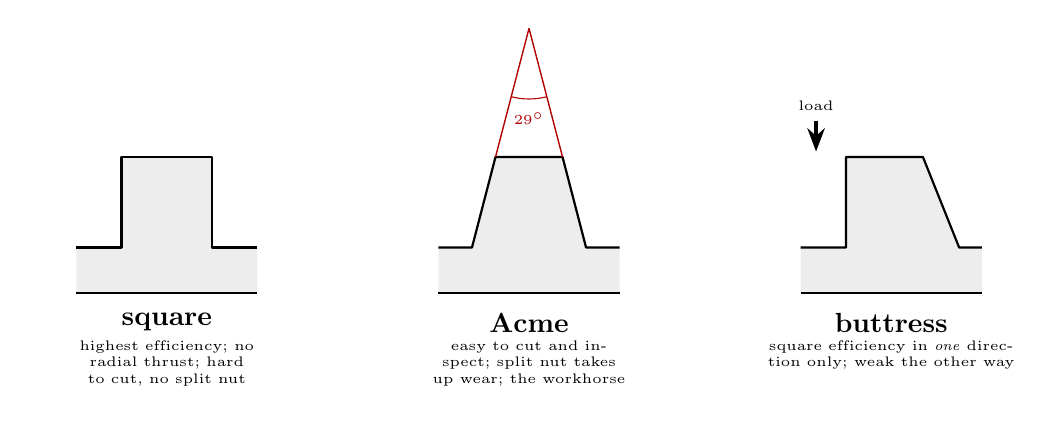
\begin{tikzpicture}[scale=1.15,>=Stealth,font=\scriptsize,line join=round]
\begin{scope}
\fill[gray!14] (0,0) -- (0.5,0) -- (0.5,1.0) -- (1.5,1.0) -- (1.5,0) -- (2.0,0)
 -- (2.0,-0.5) -- (0,-0.5) -- cycle;
\draw[thick] (0,0) -- (0.5,0) -- (0.5,1.0) -- (1.5,1.0) -- (1.5,0) -- (2.0,0);
\draw[thick] (0,-0.5) -- (2.0,-0.5);
\node[anchor=north,font=\bfseries] at (1.0,-0.62) {square};
\node[anchor=north,align=center,text width=3.3cm,font=\tiny] at (1.0,-0.92)
 {highest efficiency; no radial thrust; hard to cut, no split nut};
\end{scope}
\begin{scope}[xshift=4.0cm]
\fill[gray!14] (0,0) -- (0.37,0) -- (0.63,1.0) -- (1.37,1.0) -- (1.63,0) -- (2.0,0)
 -- (2.0,-0.5) -- (0,-0.5) -- cycle;
\draw[thick] (0,0) -- (0.37,0) -- (0.63,1.0) -- (1.37,1.0) -- (1.63,0) -- (2.0,0);
\draw[thick] (0,-0.5) -- (2.0,-0.5);
\draw[red!70!black,line width=0.5pt] (0.63,1.0) -- (1.0,2.42);
\draw[red!70!black,line width=0.5pt] (1.37,1.0) -- (1.0,2.42);
\draw[red!70!black] ($(1.0,2.42)+(255.4:0.78)$) arc (255.4:284.6:0.78);
\node[red!70!black,anchor=north,font=\tiny] at (1.0,1.60) {$29^\circ$};
\node[anchor=north,font=\bfseries] at (1.0,-0.62) {Acme};
\node[anchor=north,align=center,text width=3.3cm,font=\tiny] at (1.0,-0.92)
 {easy to cut and inspect; split nut takes up wear; the workhorse};
\end{scope}
\begin{scope}[xshift=8.0cm]
\fill[gray!14] (0,0) -- (0.5,0) -- (0.5,1.0) -- (1.35,1.0) -- (1.75,0) -- (2.0,0)
 -- (2.0,-0.5) -- (0,-0.5) -- cycle;
\draw[thick] (0,0) -- (0.5,0) -- (0.5,1.0) -- (1.35,1.0) -- (1.75,0) -- (2.0,0);
\draw[thick] (0,-0.5) -- (2.0,-0.5);
\draw[->,very thick] (0.17,1.40) -- (0.17,1.06);
\node[anchor=south,font=\tiny] at (0.17,1.41) {load};
\node[anchor=north,font=\bfseries] at (1.0,-0.62) {buttress};
\node[anchor=north,align=center,text width=3.3cm,font=\tiny] at (1.0,-0.92)
 {square efficiency in \emph{one} direction only; weak the other way};
\end{scope}
\end{tikzpicture}
}
\vfill
{\small A \SI{60}{\degree} fastener thread is a poor power screw: the steep flank generates a large
radial bursting force on the nut and wastes power in friction.}
\end{frame}

\begin{frame}{The free bodies}
\centering
\resizebox{0.86\textwidth}{!}{
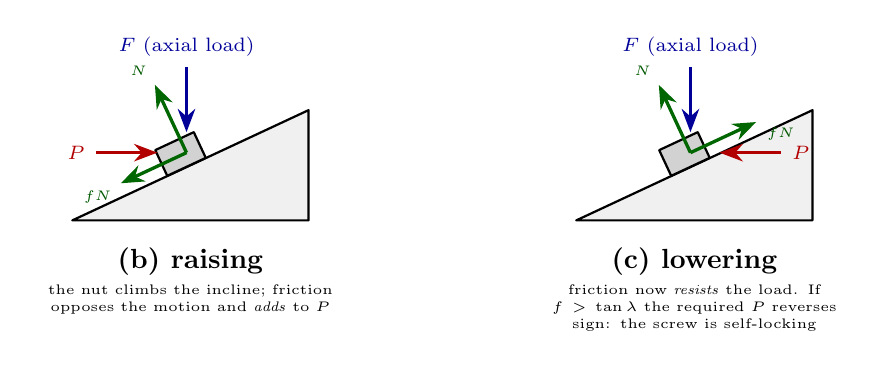
\begin{tikzpicture}[scale=1.0,>=Stealth,font=\scriptsize,line join=round]
\tikzset{frc/.style={->,very thick}}
% ---------------- (b) raising ----------------
\begin{scope}[]
\fill[gray!12] (0,0) -- (3.0,0) -- (3.0,1.40) -- cycle;
\draw[thick] (0,0) -- (3.0,0) -- (3.0,1.40) -- cycle;
\draw[thick,fill=gray!35,rotate around={25:(1.45,0.68)}] (1.18,0.68) rectangle (1.72,1.04);
\draw[frc,blue!60!black] (1.45,1.95) -- (1.45,1.12);
\node[blue!60!black,anchor=south] at (1.45,1.96) {$F$ (axial load)};
\draw[frc,red!70!black] (0.30,0.86) -- (1.08,0.86);
\node[red!70!black,anchor=east] at (0.28,0.86) {$P$};
\draw[frc,green!40!black] (1.45,0.86) -- ++(115:0.95);
\node[green!35!black,anchor=south east,font=\tiny] at (1.07,1.72) {$N$};
\draw[frc,green!40!black] (1.45,0.86) -- ++(205:0.92);
\node[green!35!black,anchor=north east,font=\tiny] at (0.62,0.50) {$fN$};
\node[anchor=north,font=\bfseries] at (1.5,-0.22) {(b) raising};
\node[anchor=north,align=center,text width=3.9cm,font=\tiny] at (1.5,-0.70)
 {the nut climbs the incline; friction opposes the motion and \emph{adds} to $P$};
\end{scope}
% ---------------- (c) lowering ----------------
\begin{scope}[xshift=6.4cm]
\fill[gray!12] (0,0) -- (3.0,0) -- (3.0,1.40) -- cycle;
\draw[thick] (0,0) -- (3.0,0) -- (3.0,1.40) -- cycle;
\draw[thick,fill=gray!35,rotate around={25:(1.45,0.68)}] (1.18,0.68) rectangle (1.72,1.04);
\draw[frc,blue!60!black] (1.45,1.95) -- (1.45,1.12);
\node[blue!60!black,anchor=south] at (1.45,1.96) {$F$ (axial load)};
\draw[frc,red!70!black] (2.60,0.86) -- (1.82,0.86);
\node[red!70!black,anchor=west] at (2.62,0.86) {$P$};
\draw[frc,green!40!black] (1.45,0.86) -- ++(115:0.95);
\node[green!35!black,anchor=south east,font=\tiny] at (1.07,1.72) {$N$};
\draw[frc,green!40!black] (1.45,0.86) -- ++(25:0.92);
\node[green!35!black,anchor=north west,font=\tiny] at (2.30,1.30) {$fN$};
\node[anchor=north,font=\bfseries] at (1.5,-0.22) {(c) lowering};
\node[anchor=north,align=center,text width=4.1cm,font=\tiny] at (1.5,-0.70)
 {friction now \emph{resists} the load. If $f>\tan\lambda$ the required $P$ reverses sign: the screw is self-locking};
\end{scope}
\end{tikzpicture}
}
\vfill
{\small Raising and lowering differ \emph{only} in the direction of the friction force. That one sign
change is the whole of self-locking.}
\end{frame}

\begin{frame}{Where $T_R$ comes from --- three steps}
Take the raising free body. Horizontal $x$, vertical $y$; incline angle $\lambda$.
\vfill
\textbf{1. Resolve.}
\[
\sum F_x:\ P - N\sin\lambda - fN\cos\lambda = 0,
\qquad
\sum F_y:\ -F + N\cos\lambda - fN\sin\lambda = 0
\]
\textbf{2. Eliminate $N$} using the $y$ equation, $N = F/(\cos\lambda - f\sin\lambda)$:
\[
P = F\,\frac{\sin\lambda + f\cos\lambda}{\cos\lambda - f\sin\lambda}
\;\;\xrightarrow[\ \div\cos\lambda\ ]{}\;\;
P = F\,\frac{\tan\lambda + f}{1 - f\tan\lambda}
\]
\textbf{3. Substitute $\tan\lambda = L/\pi d_m$ and take $T=P\,d_m/2$:}
\[
\boxed{\;T_R = \frac{F d_m}{2}\,\frac{L + \pi f d_m}{\pi d_m - f L}\;}
\]
\vfill
{\small For lowering, the friction force reverses --- change the sign of $f$ and you get $T_L$
directly. \alert{That single sign change is the entire derivation of self-locking.}}
\end{frame}

\begin{frame}{Torque to raise and to lower}
\[\boxed{\;T_R = \frac{F d_m}{2}\,\frac{L + \pi f d_m}{\pi d_m - f L}\;}\]
\vfill
\[\boxed{\;T_L = \frac{F d_m}{2}\,\frac{\pi f d_m - L}{\pi d_m + f L}\;}\]
\vfill
Look at the numerator of $T_L$.
\vfill
If $\pi f d_m > L$, the lowering torque is \alert{positive}: torque must be applied to let the load
\emph{down}. The screw will not run back on its own.
\end{frame}

\begin{frame}{Self-locking}
Divide through by $\pi d_m$, use $\tan\lambda = L/\pi d_m$, and the condition $T_L>0$ collapses to
\vfill
\[\boxed{\ f > \tan\lambda\ }\]
\vfill
\begin{alertblock}{Note what is \emph{not} in that expression}
The load. A self-locking screw holds a light load and a heavy one equally well.\\[5pt]
Not obvious, and worth remembering.
\end{alertblock}
\end{frame}

\begin{frame}{What self-locking is not}
It is a \textbf{static} property computed with a \textbf{static} friction coefficient. Three things take
it away in service:
\vfill
\begin{description}
  \item[Vibration] Transverse vibration alternately unloads the contact; effective friction falls and a
    nominally self-locking screw walks.
  \item[Lubrication] $f$ for steel on bronze may be 0.15 dry and 0.06 well greased. \alert{A screw that
    self-locks dry may not when it is serviced correctly} --- a failure mode in which doing the
    maintenance properly removes a safety property.
  \item[Wear] The contact geometry changes; the effective lead angle at the worn contact is no longer
    the design value.
\end{description}
\vfill
\centering\textbf{Self-locking is never accepted as the sole retention feature on a flight-critical adjustment.}
\end{frame}

\begin{frame}{Self-locking: a feel for the numbers}
The boundary is simply $\lambda_{\max} = \arctan f$.
\vfill
\centering\small
\begin{tabular}{@{}lcccc@{}}
\toprule
 & & \multicolumn{3}{c}{self-locking?}\\
\cmidrule(l){3-5}
$\lambda$ & $\tan\lambda$ & $f=0.08$ & $f=0.15$ & $f=0.25$\\
 & & {\footnotesize greased} & {\footnotesize dry steel/bronze} & {\footnotesize dry, rough}\\
\midrule
\SI{2}{\degree} & 0.035 & yes & yes & yes\\
\SI{4}{\degree} & 0.070 & yes & yes & yes\\
\SI{6}{\degree} & 0.105 & \alert{no} & yes & yes\\
\SI{10}{\degree} & 0.176 & \alert{no} & \alert{no} & yes\\
\SI{15}{\degree} & 0.268 & \alert{no} & \alert{no} & \alert{no}\\
\midrule
$\lambda_{\max}$ & & \SI{4.6}{\degree} & \SI{8.5}{\degree} & \SI{14.0}{\degree}\\
\bottomrule
\end{tabular}
\vfill
\raggedright
{\small Example 5.1 sits at $\lambda=\SI{3.77}{\degree}$ --- locked in all three columns.
\alert{A screw at \SI{6}{\degree} locks dry and releases when greased.}}
\end{frame}

\begin{frame}{Efficiency --- and the price of self-locking}
\centering
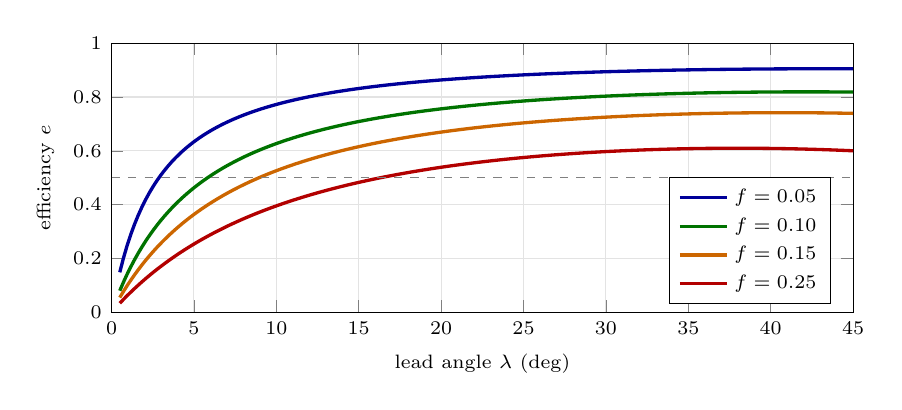
\begin{tikzpicture}
\begin{axis}[width=11.0cm,height=5.0cm,xlabel={lead angle $\lambda$ (deg)},
  ylabel={efficiency $e$},xmin=0,xmax=45,ymin=0,ymax=1,
  grid=both,grid style={gray!22},legend pos=south east,
  label style={font=\scriptsize},tick label style={font=\scriptsize},
  legend style={font=\scriptsize}]
\addplot[domain=0.5:45,samples=200,very thick,blue!60!black]
  {tan(x)*(1-0.05*tan(x))/(tan(x)+0.05)}; \addlegendentry{$f=0.05$}
\addplot[domain=0.5:45,samples=200,very thick,green!45!black]
  {tan(x)*(1-0.10*tan(x))/(tan(x)+0.10)}; \addlegendentry{$f=0.10$}
\addplot[domain=0.5:45,samples=200,very thick,orange!80!black]
  {tan(x)*(1-0.15*tan(x))/(tan(x)+0.15)}; \addlegendentry{$f=0.15$}
\addplot[domain=0.5:45,samples=200,very thick,red!70!black]
  {tan(x)*(1-0.25*tan(x))/(tan(x)+0.25)}; \addlegendentry{$f=0.25$}
\addplot[dashed,gray,domain=0:45,samples=2]{0.5};
\end{axis}
\end{tikzpicture}
\vfill
{\small $e = \dfrac{\tan\lambda\,(1-f\tan\lambda)}{\tan\lambda+f}$ \quad---\quad a self-locking screw
($\tan\lambda<f$) lives on the steep left-hand part of its curve. \alert{Self-locking costs you at
least half the input power.} There is no way around it with a plain thread.}
\end{frame}

\begin{frame}{Two corrections you must not forget}
\begin{columns}[T]
\begin{column}{0.49\textwidth}
\begin{block}{Flank angle (Acme)}
Replace $f$ by $f\sec\alpha$, with $\alpha=\SI{14.5}{\degree}$:
\[ \sec\alpha = 1.033 \]
A \SI{3}{\percent} penalty on the friction term --- which makes Acme slightly \emph{more} reliably
self-locking than square.
\end{block}
\end{column}
\begin{column}{0.49\textwidth}
\begin{block}{Collar friction}
\[ T_c = \frac{F f_c d_c}{2} \]
Often \alert{larger than the thread term itself}.\\[5pt]
First place to attack for efficiency: a rolling thrust bearing takes $f_c$ from $\approx 0.12$ to
$\approx 0.005$.
\end{block}
\end{column}
\end{columns}
\end{frame}

\begin{frame}{Example 5.1 --- a square-thread screw}
$d=\SI{32}{mm}$, $p=\SI{6}{mm}$ single start, $F=\SI{6.8}{kN}$, $f=0.15$; plain collar
$d_c=\SI{40}{mm}$, $f_c=0.12$.
\vfill
$d_m = \SI{29}{mm}$, \ $\tan\lambda = 6/(\pi\cdot 29) = 0.0659$, \ $\lambda = \SI{3.77}{\degree}$
$\Rightarrow$ $f=0.15 > 0.0659$: \textbf{self-locking}.
\vfill
\centering\small
\begin{tabular}{@{}lccc@{}}
\toprule
 & thread (\si{N.m}) & collar (\si{N.m}) & total (\si{N.m})\\
\midrule
Raise $T_R$ & 21.5 & 16.3 & \textbf{37.8}\\
Lower $T_L$ & 8.2 & 16.3 & 24.5\\
\bottomrule
\end{tabular}
\vfill
\raggedright
Efficiency: thread alone \SI{30.2}{\percent}; \ \alert{overall \SI{17.2}{\percent}}.
\vfill
{\small \SI{83}{\percent} of the input becomes heat --- and more than half the loss is in the
\emph{collar}, not the thread.}
\end{frame}

\begin{frame}{Where the torque actually goes --- Example 5.1}
\centering
\resizebox{0.92\textwidth}{!}{
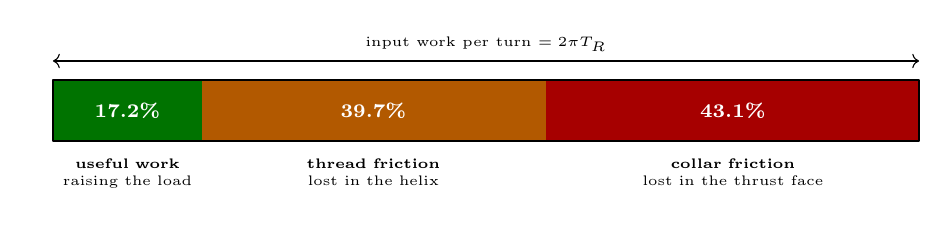
\begin{tikzpicture}[scale=1.0,font=\scriptsize,line join=round]
\def\W{11.0}
\fill[green!45!black] (0,0) rectangle (0.172*\W,0.78);
\fill[orange!70!black] (0.172*\W,0) rectangle (0.569*\W,0.78);
\fill[red!65!black] (0.569*\W,0) rectangle (\W,0.78);
\draw[thick] (0,0) rectangle (\W,0.78);
\node[white,font=\bfseries\scriptsize] at (0.086*\W,0.39) {17.2\%};
\node[white,font=\bfseries\scriptsize] at (0.370*\W,0.39) {39.7\%};
\node[white,font=\bfseries\scriptsize] at (0.785*\W,0.39) {43.1\%};
\node[anchor=north,align=center,font=\tiny,text width=2.3cm] at (0.086*\W,-0.10)
  {\textbf{useful work}\\ raising the load};
\node[anchor=north,align=center,font=\tiny,text width=3.0cm] at (0.370*\W,-0.10)
  {\textbf{thread friction}\\ lost in the helix};
\node[anchor=north,align=center,font=\tiny,text width=3.0cm] at (0.785*\W,-0.10)
  {\textbf{collar friction}\\ lost in the thrust face};
\draw[<->] (0,1.02) -- (\W,1.02) node[midway,above,font=\tiny]
  {input work per turn $=2\pi T_R$};
\end{tikzpicture}
}
\vfill
\raggedright
\begin{itemize}
  \item The \alert{collar} loses more than the thread does. Attack it first --- a rolling thrust
        bearing takes $f_c$ from 0.12 to 0.005 and nearly doubles the overall efficiency.
  \item The thread friction is \emph{not} waste you can design out: it is the same friction that makes
        the screw self-locking. Removing it removes the property you wanted.
\end{itemize}
\vfill
{\small A power screw is a deliberately inefficient machine. If that offends you, you have not yet
understood what you are buying with the inefficiency.}
\end{frame}

\begin{frame}{What actually sets the life: bearing pressure}
\[\boxed{\ p_b = \frac{F}{\pi d_m h\, n_t}\ }\]
\vfill
Safe values for slow screws: steel on bronze \SIrange{17}{24}{MPa}; steel on cast iron
\SIrange{13}{18}{MPa}; steel on steel \SIrange{7}{12}{MPa}.
\vfill
\alert{These are \emph{wear} limits, not strength limits}, and they fall as sliding speed rises.
\vfill
\begin{alertblock}{Load sharing}
The first engaged thread may take \SIrange{30}{40}{\percent} of the total. Adding threads past about
ten buys almost nothing.
\end{alertblock}
\end{frame}

\begin{frame}{Example 5.2 --- wear is self-accelerating}
Acme jackscrew: $d=\SI{40}{mm}$, $p=\SI{6}{mm}$, $F=\SI{30}{kN}$, bronze nut, $n_t=8$.\\
Areas scale with the remaining flank thickness, so stresses scale as $1/(1-x)$.
\vfill
\centering
\begin{tabular}{@{}lcc@{}}
\toprule
Thread thickness lost & $p_b$ (\si{MPa}) & $\tau$ (\si{MPa})\\
\midrule
0 (as new) & 10.8 & 9.9\\
\SI{50}{\percent} & 21.5 & 19.9\\
\SI{90}{\percent} & \alert{\textbf{107.5}} & \alert{\textbf{99.5}}\\
\bottomrule
\end{tabular}
\vfill
\raggedright
At \SI{50}{\percent} the bearing pressure has already passed the safe value --- so the wear rate is now
climbing.
\vfill
\centering\textbf{The part looks fine for most of its life, then deteriorates very quickly.}
\end{frame}


\begin{frame}{A power screw is also a column}
\centering
\resizebox{!}{4.4cm}{% A jackscrew is a column whose length changes as it works.
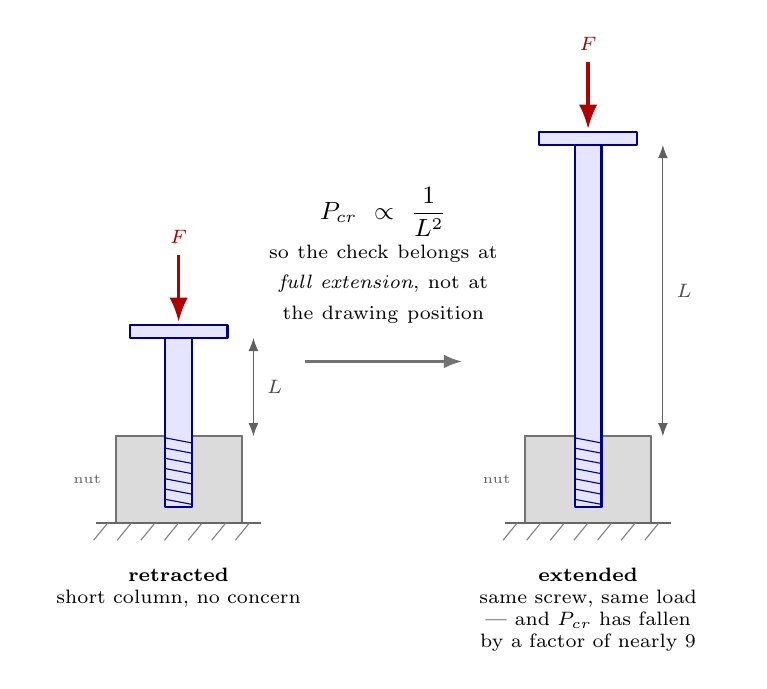
\begin{tikzpicture}[>=Latex,line join=round]
\tikzset{
  scr/.style={fill=blue!10,draw=blue!55!black,thick},
  hous/.style={fill=black!14,draw=black!55,thick},
  ld/.style={->,red!70!black,line width=1.3pt},
  dimn/.style={<->,gray!75!black,thin},
  lb/.style={font=\scriptsize,align=center,text width=3.6cm,anchor=north},
  ttl/.style={font=\small\bfseries,anchor=south}
}
% \jack{x}{free length}{label}
\newcommand{\jack}[3]{%
  % housing / nut block
  \fill[hous] (#1-0.80,0) rectangle (#1+0.80,1.10);
  \draw[black!55,thick] (#1-0.80,0) rectangle (#1+0.80,1.10);
  \node[font=\tiny,text=black!60,anchor=east] at (#1-0.86,0.55) {nut};
  % ground
  \draw[black!60,thick] (#1-1.05,0) -- (#1+1.05,0);
  \foreach \k in {-0.9,-0.6,...,0.95}{\draw[black!50,thin] (#1+\k,0) -- (#1+\k-0.18,-0.22);}
  % screw, from inside the nut up through the free length
  \draw[scr] (#1-0.17,0.20) rectangle (#1+0.17,1.10+#2);
  \foreach \k in {0,1,...,40}{
    \pgfmathsetmacro\yy{0.30+0.13*\k}
    \ifdim\yy pt<1.10pt \draw[blue!55!black,thin] (#1-0.17,\yy) -- (#1+0.17,\yy-0.065);\fi}
  % platform and load
  \fill[blue!10,draw=blue!55!black,thick] (#1-0.62,1.10+#2) rectangle (#1+0.62,1.26+#2);
  \draw[ld] (#1,2.15+#2) -- (#1,1.30+#2);
  \node[font=\scriptsize,text=red!70!black,anchor=south] at (#1,2.18+#2) {$F$};
  % free length dimension
  \draw[dimn] (#1+0.95,1.10) -- (#1+0.95,1.10+#2);
  \node[font=\scriptsize,anchor=west,text=gray!60!black] at (#1+1.00,1.10+#2/2) {$L$};
  \node[lb] at (#1,-0.45) {#3};
}

\jack{0}{1.25}{\textbf{retracted}\\ short column, no concern}
\jack{5.2}{3.70}{\textbf{extended}\\ same screw, same load --- and
$P_{cr}$ has fallen by a factor of nearly $9$}

% the point, between the two
\node[font=\small,align=center,text width=3.4cm] at (2.6,3.4)
 {$P_{cr}\propto \dfrac{1}{L^{2}}$\\[3pt] \scriptsize so the check belongs at \emph{full extension}, not at the drawing position};
\draw[->,black!55,thick] (1.60,2.05) -- (3.60,2.05);

\end{tikzpicture}
}
\vfill
\raggedright
Everything so far sized the screw against \textbf{thread} failure. A long screw in compression fails
in a way that has nothing to do with its thread --- and for a jackscrew this is often the check that
sets the diameter.
\end{frame}

\begin{frame}{Two traps before you substitute anything}
\begin{columns}[T]
\begin{column}{0.48\textwidth}
\begin{alertblock}{1. Use the \emph{root} diameter}
\[ I=\frac{\pi d_r^{4}}{64},\qquad k=\frac{d_r}{4} \]
The crests carry nothing in bending.
\vspace{2pt}
{\footnotesize On our \SI{32}{mm}/\SI{6}{mm} screw, using $d$ instead of $d_r$ overstates $I$ by
$(32/26)^4 = \mathbf{2.3}$ --- more than twice the buckling load you actually have.}
\end{alertblock}
\end{column}
\begin{column}{0.48\textwidth}
\begin{alertblock}{2. Use the length at \emph{full extension}}
\[ P_{cr}=\frac{C\pi^{2}EI}{L^{2}} \]
The nut moves, so $L$ is a design \emph{variable}.
\vspace{2pt}
{\footnotesize $P_{cr}\propto 1/L^2$, so the worst case is always the fully extended one --- which
is the position nobody draws.}
\end{alertblock}
\end{column}
\end{columns}
\vfill
\centering\footnotesize
$C=0.25$ fixed--free \ $\cdot$ \ $C=1$ pinned--pinned \ $\cdot$ \ $C=2$ fixed--pinned \ $\cdot$ \
$C=4$ fixed--fixed
\end{frame}

\begin{frame}{Example 5.6 --- how long may the screw of Example 5.1 be?}
$d=\SI{32}{mm}$, $p=\SI{6}{mm}$, steel, $F=\SI{6.8}{kN}$, buckling factor 3 so
$P_{cr}=\SI{20.4}{kN}$. \ $d_r=\SI{26}{mm}$, $I=\SI{2.243e-8}{m^4}$, $k=\SI{6.5}{mm}$.
\vfill
\centering\small
\begin{tabular}{@{}lccccl@{}}
\toprule
End condition & $C$ & $L$ at SF\,3 & $L/k$ & $(L/k)_1$ & Valid?\\
\midrule
fixed--free & 0.25 & \SI{749}{mm} & 115 & 51 & Euler\\
pinned--pinned & 1.0 & \SI{1499}{mm} & 231 & 101 & Euler\\
fixed--pinned & 2.0 & \SI{2120}{mm} & 326 & 143 & Euler\\
\bottomrule
\end{tabular}
\vfill
\raggedright
\begin{block}{Read the first two rows together}
Same screw, same load, same factor. Supporting the far end --- a guide bush, a second bearing, a
telescoping tube --- \textbf{doubles the length you may use}. A cheap part buying a metre of stroke,
and the reason actuator screws so often run inside a tube.
\end{block}
\end{frame}

\begin{frame}{And if it spins fast: whirling}
A rotating screw is also a shaft, with a first critical speed at which it whirls:
\[
\omega_{cr}=\left(\frac{\pi}{L}\right)^{2}\sqrt{\frac{EI}{\rho A}}
\]
\vfill
For the screw above at $L=\SI{749}{mm}$: about \alert{\SI{5600}{rpm}} --- at which the nut would
travel \SI{560}{mm/s}.
\vfill
\begin{alertblock}{No Acme jack goes near that --- which is the point}
\textbf{Whirling governs ball screws, not jackscrews.} The ball screw is efficient, so it gets
driven fast; speed is the one thing the Acme screw's own inefficiency protects it from.
\vspace{2pt}
Check it whenever you replace an Acme screw with a ball screw \textbf{and keep the same motor}.
\end{alertblock}
\end{frame}

\begin{frame}{Ball screws}
\centering
\resizebox{!}{3.6cm}{
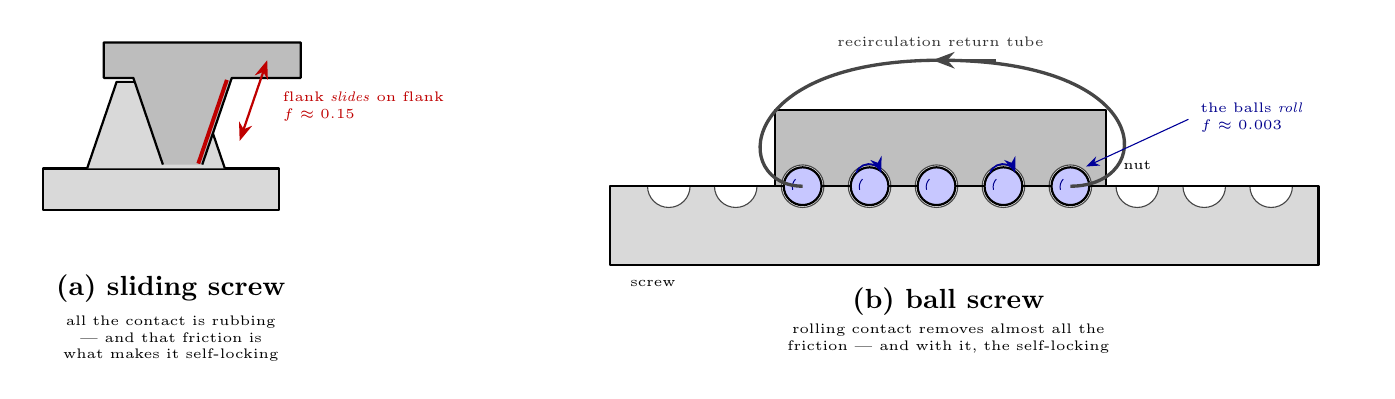
\begin{tikzpicture}[scale=1.0,>=Stealth,font=\scriptsize,line join=round]
%========== (a) sliding screw: flank on flank ==========
\begin{scope}[scale=1.25,yshift=0.12cm]
\fill[gray!30] (0,0) -- (2.4,0) -- (2.4,0.42) -- (0,0.42) -- cycle;
\draw[thick] (0,0) rectangle (2.4,0.42);
\fill[gray!30] (0.45,0.42) -- (0.75,1.30) -- (1.55,1.30) -- (1.85,0.42) -- cycle;
\draw[thick] (0.45,0.42) -- (0.75,1.30) -- (1.55,1.30) -- (1.85,0.42);
\fill[gray!52] (1.62,0.46) -- (1.92,1.34) -- (2.62,1.34) -- (2.62,1.70) -- (0.62,1.70)
  -- (0.62,1.34) -- (0.92,1.34) -- (1.22,0.46) -- cycle;
\draw[thick] (1.62,0.46) -- (1.92,1.34) -- (2.62,1.34) -- (2.62,1.70) -- (0.62,1.70)
  -- (0.62,1.34) -- (0.92,1.34) -- (1.22,0.46);
\draw[red!75!black,line width=1.4pt] (1.58,0.47) -- (1.87,1.32);
\draw[<->,red!75!black,thick] (2.00,0.70) -- (2.28,1.52);
\node[red!75!black,anchor=west,align=left,font=\tiny,text width=2.3cm] at (2.34,1.05)
  {flank \emph{slides} on flank\\ $f \approx 0.15$};
\node[anchor=north,font=\bfseries] at (1.3,-0.56) {(a) sliding screw};
\node[anchor=north,align=center,font=\tiny,text width=3.4cm] at (1.3,-0.98)
  {all the contact is rubbing --- and that friction is what makes it self-locking};
\end{scope}
%========== (b) ball screw: recirculating rolling contact ==========
\begin{scope}[xshift=7.2cm]
% screw shaft with grooves
\begin{scope}
\clip (0,-0.55) rectangle (9.0,0.45);
\fill[gray!30] (0,-0.55) rectangle (9.0,0.45);
\foreach \x in {0.75,1.6,2.45,3.3,4.15,5.0,5.85,6.7,7.55,8.4}{
  \fill[white] (\x,0.45) circle (0.27); \draw[gray!55!black,line width=0.4pt] (\x,0.45) circle (0.27);}
\end{scope}
\draw[thick] (0,-0.55) rectangle (9.0,0.45);
\node[anchor=north,font=\tiny] at (0.55,-0.62) {screw};
% nut body with matching grooves
\begin{scope}
\clip (2.1,0.45) rectangle (6.3,1.42);
\fill[gray!50] (2.1,0.45) rectangle (6.3,1.42);
\foreach \x in {2.45,3.3,4.15,5.0,5.85}{
  \fill[white] (\x,0.45) circle (0.27); \draw[gray!55!black,line width=0.4pt] (\x,0.45) circle (0.27);}
\end{scope}
\draw[thick] (2.1,0.45) rectangle (6.3,1.42);
\node[anchor=west,font=\tiny] at (6.4,0.72) {nut};
% balls
\foreach \x in {2.45,3.3,4.15,5.0,5.85}{
  \draw[thick,fill=blue!22] (\x,0.45) circle (0.24);
  \draw[blue!55!black,line width=0.35pt] (\x-0.09,0.54) arc (135:195:0.14);}
% rotation of the balls
\foreach \x in {3.3,5.0}{\draw[->,blue!60!black,line width=0.6pt] (\x-0.17,0.62) arc (160:20:0.17);}
% recirculation return tube
\draw[very thick,gray!55!black]
  (5.85,0.45) .. controls (6.95,0.45) and (6.95,2.05) .. (4.20,2.05)
  .. controls (1.55,2.05) and (1.55,0.45) .. (2.45,0.45);
\draw[->,gray!55!black,line width=1.1pt] (4.9,2.05) -- (4.1,2.05);
\node[anchor=south,font=\tiny,gray!40!black] at (4.2,2.10) {recirculation return tube};
\draw[->,blue!60!black] (7.35,1.30) -- (6.05,0.70);
\node[blue!55!black,anchor=west,align=left,font=\tiny,text width=2.0cm] at (7.38,1.32)
  {the balls \emph{roll}\\ $f\approx0.003$};
\node[anchor=north,font=\bfseries] at (4.3,-0.72) {(b) ball screw};
\node[anchor=north,align=center,font=\tiny,text width=6.4cm] at (4.3,-1.18)
  {rolling contact removes almost all the friction --- and with it, the self-locking};
\end{scope}
\end{tikzpicture}
}
\vfill
\raggedright
\begin{columns}[T]
\begin{column}{0.46\textwidth}
\begin{itemize}\small
  \item efficiency $\approx \SI{90}{\percent}$
  \item $f$ so small that $f<\tan\lambda$ \alert{always}
\end{itemize}
\end{column}
\begin{column}{0.50\textwidth}
{\small Wonderful for a powered actuator. \alert{Dangerous for a holding one} --- a ball screw
back-drives under load, so it must be fitted with a brake or a no-back.}
\end{column}
\end{columns}
\vfill
{\small Aerospace ball screws go where the duty cycle is high and the drive holds the load. Sliding
Acme screws survive where \emph{the screw itself} must hold.}
\end{frame}


\section{Materials and environment}

\begin{frame}{Four ways to lose the preload you just set}
Everything so far treated the fastener as elastic steel in a room. It sits in an assembly of other
metals, in weather, through a temperature range, for decades.
\vfill
\begin{columns}[T]
\begin{column}{0.235\textwidth}
\begin{block}{Galling}
the preload never \textbf{arrives}
\end{block}
\end{column}
\begin{column}{0.235\textwidth}
\begin{block}{Galvanic}
the joint is \textbf{eaten} from the fastener out
\end{block}
\end{column}
\begin{column}{0.235\textwidth}
\begin{block}{Temperature}
preload \textbf{moves}, both ways, after you leave
\end{block}
\end{column}
\begin{column}{0.235\textwidth}
\begin{block}{Composites}
every habit from aluminium is \textbf{wrong}
\end{block}
\end{column}
\end{columns}
\vfill
\centering
None of the four appears anywhere in the stress calculation.
\end{frame}

\begin{frame}{Galling: the fastener that will neither tighten nor come off}
Galling is \textbf{solid-phase welding}. The oxide film is wiped off the flanks, clean metal meets
clean metal, and the surfaces cold-weld, tear and transfer material.
\vfill
\begin{columns}[T]
\begin{column}{0.46\textwidth}
\begin{alertblock}{Why it is so bad on a thread}
The torque you read is no longer friction --- it is the torque to shear welded junctions. $K$ is
meaningless and \textbf{the preload never arrives}.
\vspace{2pt}
The nut then seizes part way down: you can neither tighten it nor remove it. The way out is to cut
it off, which damages the hole.
\end{alertblock}
\end{column}
\begin{column}{0.50\textwidth}
\begin{block}{The offenders are what aerospace likes most}
300-series CRES, titanium, aluminium --- soft-ish, work-hardening, and carrying a tenacious oxide
thin enough to wipe off and keen enough to re-weld. \textbf{Like-on-like is the worst case.}
\vspace{2pt}
{\footnotesize Fixes: avoid like-on-like \ $\cdot$ \ MoS$_2$ dry film (``prevents seizing and
galling'') \ $\cdot$ \ silver plate \ $\cdot$ \ passivate CRES \ $\cdot$ \ \textbf{run the nut on
slowly}.}
\end{block}
\end{column}
\end{columns}
\vfill
\centering
And then \alert{change the torque value} --- you have just changed the friction.
\end{frame}

\begin{frame}{Galvanic: the fastener is always the small part}
\begin{columns}[T]
\begin{column}{0.26\textwidth}
\centering
\resizebox{!}{5.6cm}{% Simplified galvanic series, with the three pairings that matter in airframes.
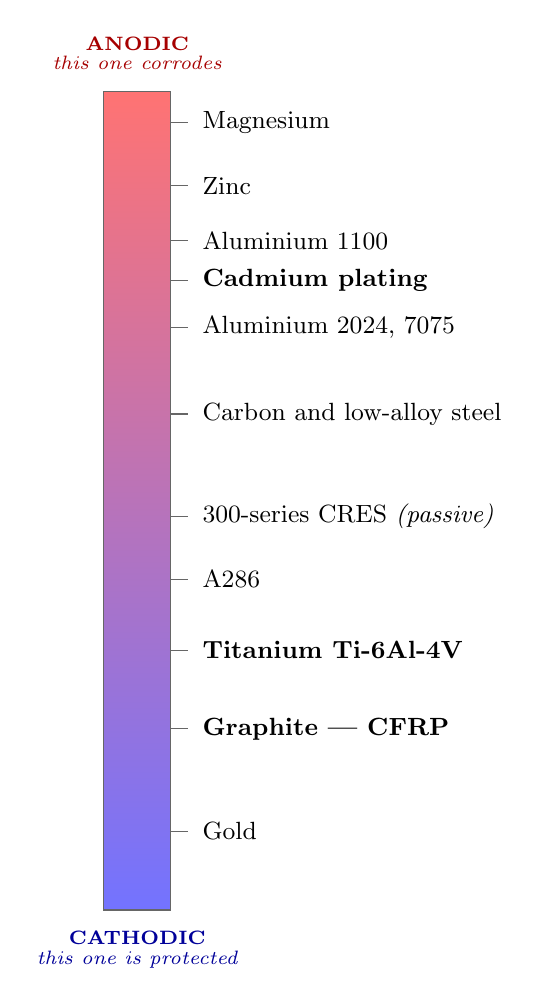
\begin{tikzpicture}[>=Latex]
\tikzset{
  mt/.style={font=\small,anchor=west},
  tick/.style={black!60,thin},
  good/.style={draw=green!45!black,line width=1.1pt},
  bad/.style={draw=red!70!black,line width=1.1pt},
  gl/.style={font=\scriptsize,align=left,text width=5.0cm,anchor=west,text=green!35!black},
  bl/.style={font=\scriptsize,align=left,text width=5.0cm,anchor=west,text=red!65!black}
}
\def\W{0.85}

% ---- the strip ----
\shade[top color=red!55,bottom color=blue!55] (0,0) rectangle (\W,10.4);
\draw[black!60] (0,0) rectangle (\W,10.4);
\node[font=\scriptsize\bfseries,text=red!65!black,anchor=south,align=center] at (\W/2,10.55) {ANODIC\\[-1pt] \mdseries\itshape this one corrodes};
\node[font=\scriptsize\bfseries,text=blue!60!black,anchor=north,align=center] at (\W/2,-0.15) {CATHODIC\\[-1pt] \mdseries\itshape this one is protected};

% ---- members ----
\foreach \y/\n in {
  10.0/{Magnesium},
   9.2/{Zinc},
   8.5/{Aluminium 1100},
   8.0/{\textbf{Cadmium plating}},
   7.4/{Aluminium 2024, 7075},
   6.3/{Carbon and low-alloy steel},
   5.0/{300-series CRES \emph{(passive)}},
   4.2/{A286},
   3.3/{\textbf{Titanium Ti-6Al-4V}},
   2.3/{\textbf{Graphite --- CFRP}},
   1.0/{Gold}}
{
  \draw[tick] (\W,\y) -- (\W+0.22,\y);
  \node[mt] at (\W+0.28,\y) {\n};
}

\end{tikzpicture}
}
\end{column}
\begin{column}{0.70\textwidth}
\begin{block}{Rule 1 --- separation}
``The farther apart two materials are in the \dots\ list, the greater the galvanic action between
them.'' Separation sets the driving voltage.
\end{block}
\begin{alertblock}{Rule 2 --- area (the one students forget)}
``Because the anode is eroded in a galvanic cell, \emph{it should be the larger mass in the cell}.''
\vspace{2pt}
A large anode corrodes slowly and evenly; a \textbf{small} anode takes the whole current and is
eaten quickly, in one place.
\end{alertblock}
\vspace{2pt}
{\footnotesize A fastener is always the small part. Therefore \textbf{the fastener must be the
cathode} --- and that one sentence explains almost all aerospace fastener material practice.}
\end{column}
\end{columns}
\end{frame}

\begin{frame}{Which fastener goes in which structure}
\centering\footnotesize
\begin{tabular}{@{}p{2.3cm}p{2.9cm}p{7.6cm}@{}}
\toprule
Structure & Fastener & Why\\
\midrule
Aluminium alloy & cadmium-plated alloy steel & cadmium sits \emph{beside} the aluminium alloys, so
the plating makes a steel fastener look electrochemically like the structure. \textbf{That is what
cadmium is for.}\\[2pt]
Steel assembly & CRES & the large steel assembly is the anode. The reverse --- carbon steel
fasteners in a stainless assembly --- RP-1228 calls \emph{poor design practice}.\\[2pt]
CFRP & Ti-6Al-4V, or A286 & titanium is close to graphite. Aluminium is ``not recommended'':
``the small anode \dots\ to large cathode (carbon composite) accelerates the corrosion''.\\
\bottomrule
\end{tabular}
\vfill
\raggedright
\begin{alertblock}{Two more lines for the drawing}
\textbf{Wet installation.} A cell needs an electrolyte path --- sealant breaks it, and seals the
hole against moisture at the same time.
\vspace{2pt}
\textbf{Cadmium's own limits.} It embrittles, so plated high-strength steel is \textbf{baked after
plating}; and it stops at about \SI{450}{\degree F}. Above that, silver --- but never against
aluminium or magnesium.
\end{alertblock}
\end{frame}

\begin{frame}{Temperature: the joint that tightens itself}
A steel bolt through aluminium members is two expansion coefficients in series. Heat it and the
members grow faster than the bolt can stretch: \textbf{the preload rises}. Cool it and it falls.
\[
\Delta F_i = \frac{(\alpha_m - \alpha_b)\,L\,\Delta T}{\dfrac{1}{k_b}+\dfrac{1}{k_m}}
\]
\vfill
\begin{columns}[T]
\begin{column}{0.46\textwidth}
\begin{block}{The M10 joint, aluminium members}
$k_m = \SI{671}{kN/mm}$, so $C = \mathbf{0.42}$ --- it was 0.20 with steel. Softer members have
already doubled the bolt's share.
\end{block}
\end{column}
\begin{column}{0.50\textwidth}
\begin{alertblock}{$+\SI{100}{\degree C}$}
$\Delta L = \SI{0.0357}{mm}$, $\Delta F_i = \SI{10.0}{kN}$
\vspace{2pt}
$F_i:\ 36.1 \to \SI{46.1}{kN} = \mathbf{96\%\ \text{of proof}}$ --- the entire margin, gone, with
nothing left for the external load. At $-\SI{100}{\degree C}$: a \SI{28}{\percent} loss of clamp.
\end{alertblock}
\end{column}
\end{columns}
\end{frame}

\begin{frame}{What to do about temperature}
\begin{columns}[T]
\begin{column}{0.48\textwidth}
\begin{block}{Check both ends}
of the temperature range --- not the assembly temperature.
\end{block}
\begin{block}{Lengthen the bolt}
$\Delta F_i$ falls as the grip's compliance rises. A short stiff bolt is the wrong answer
\textbf{twice}: for fatigue, and for temperature.
\end{block}
\end{column}
\begin{column}{0.48\textwidth}
\begin{alertblock}{Matching is not always better}
A titanium bolt ($\alpha\approx\SI{8.6e-6}{/\degree C}$) in an aluminium fitting is \textbf{worse},
not better.
\end{alertblock}
\begin{block}{Know which way it goes}
Steel in aluminium \textbf{gains} preload when hot --- dangerous at the top of the range. Aluminium
in steel would lose it.
\end{block}
\end{column}
\end{columns}
\end{frame}

\begin{frame}{Fasteners in composites}
A laminate does not yield, so it will not redistribute bearing stress. It is weak through the
thickness. And it is conductive and strongly \textbf{cathodic}.
\vfill
\begin{columns}[T]
\begin{column}{0.48\textwidth}
\begin{alertblock}{Material}
Titanium or A286 --- \textbf{never} aluminium or cadmium-plated steel.
\end{alertblock}
\begin{alertblock}{No interference fit}
Rivets ``expand into an interference fit, and this may cause delamination damage around the hole''.
What improves fatigue life in aluminium is \textbf{damage} in a laminate.
\end{alertblock}
\end{column}
\begin{column}{0.48\textwidth}
\begin{alertblock}{Hole quality is structural}
Worn or wrong drills give chipping, fibre pull-out and \textbf{exit-side delamination} --- inside
the laminate, invisible from either face.
\end{alertblock}
\begin{alertblock}{Spread the load}
Large heads, washers under head \emph{and} nut. ``There is a decreased bearing strength when there
are countersunk holes'' --- the $\le\tfrac23 t$ rule is a \textbf{minimum} here, not a sufficient
condition.
\end{alertblock}
\end{column}
\end{columns}
\end{frame}

\begin{frame}{The summary you can take into a design review}
\centering
\large
The bolt calculation gives you a number.\\[4pt]
\alert{The environment decides whether you keep it.}
\vfill
\raggedright\normalsize
\begin{itemize}
\item \textbf{Galling} stops the preload arriving.
\item \textbf{Galvanic action} eats the joint from the fastener outwards --- because the fastener is
  always the small part.
\item \textbf{Temperature} moves the preload in both directions after you have left.
\item \textbf{A laminate} will not forgive any of the habits you learned on aluminium.
\end{itemize}
\vfill
\centering
Each of these is a \textbf{line on the drawing}, not a judgement for the shop floor.
\end{frame}

\section{The stabiliser trim jackscrew}

\begin{frame}{The largest power screw on the aeroplane}
The horizontal stabiliser is trimmed by pivoting the whole surface.
\vfill
A single Acme jackscrew, driven by two independent motors. The nut is attached to the stabiliser; the
screw is restrained at the airframe end.
\vfill
It is loaded for the whole flight, and it moves slowly and continuously.
\vfill
\begin{alertblock}{A deliberate wear point}
The bronze Acme nut is designed to be the sacrificial element. It is \emph{expected} to wear and be
replaced --- with grease to slow the wear, and a periodic \textbf{end-play check} to measure how far it
has gone.
\end{alertblock}
\end{frame}

\begin{frame}{What an end-play check actually measures}
\centering
\resizebox{!}{3.5cm}{
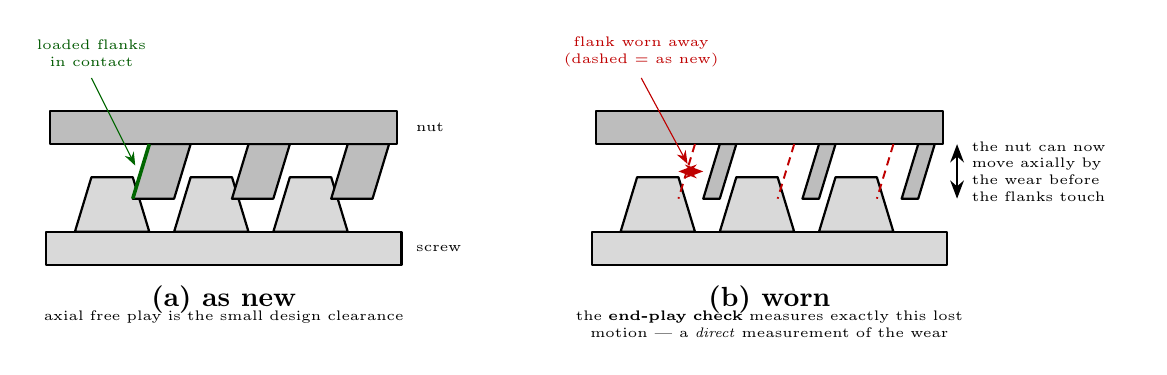
\begin{tikzpicture}[scale=1.05,>=Stealth,font=\scriptsize,line join=round]
\tikzset{scr/.style={thick,fill=gray!30},nut/.style={thick,fill=gray!52}}
% ================= (a) as new =================
\begin{scope}
\fill[gray!30] (0,0) rectangle (4.3,0.40); \draw[thick] (0,0) rectangle (4.3,0.40);
\node[anchor=west,font=\tiny] at (4.36,0.20) {screw};
\foreach \x in {0.35,1.55,2.75}{
  \draw[scr] (\x,0.40) -- (\x+0.20,1.06) -- (\x+0.70,1.06) -- (\x+0.90,0.40) -- cycle;}
\fill[gray!52] (0.05,1.46) rectangle (4.25,1.86); \draw[thick] (0.05,1.46) rectangle (4.25,1.86);
\node[anchor=west,font=\tiny] at (4.36,1.66) {nut};
\foreach \x in {1.25,2.45,3.65}{
  \draw[nut] (\x,1.46) -- (\x-0.20,0.80) -- (\x+0.30,0.80) -- (\x+0.50,1.46) -- cycle;}
\draw[green!40!black,line width=1.3pt] (1.05,0.80) -- (1.25,1.46);
\draw[->,green!40!black] (0.55,2.26) -- (1.08,1.20);
\node[green!35!black,anchor=south,font=\tiny,align=center] at (0.55,2.28)
  {loaded flanks\\ in contact};
\node[anchor=north,font=\bfseries] at (2.15,-0.14) {(a) as new};
\node[anchor=north,align=center,font=\tiny,text width=4.6cm] at (2.15,-0.44)
  {axial free play is the small design clearance};
\end{scope}
% ================= (b) worn =================
\begin{scope}[xshift=6.6cm]
\fill[gray!30] (0,0) rectangle (4.3,0.40); \draw[thick] (0,0) rectangle (4.3,0.40);
\foreach \x in {0.35,1.55,2.75}{
  \draw[scr] (\x,0.40) -- (\x+0.20,1.06) -- (\x+0.70,1.06) -- (\x+0.90,0.40) -- cycle;}
\fill[gray!52] (0.05,1.46) rectangle (4.25,1.86); \draw[thick] (0.05,1.46) rectangle (4.25,1.86);
% worn nut teeth: the loaded flank has receded
\foreach \x in {1.25,2.45,3.65}{
  \draw[nut] (\x+0.30,1.46) -- (\x+0.10,0.80) -- (\x+0.30,0.80) -- (\x+0.50,1.46) -- cycle;
  \draw[red!75!black,densely dashed,line width=0.7pt] (\x,1.46) -- (\x-0.20,0.80);}
\draw[<->,red!75!black,thick] (1.05,1.13) -- (1.35,1.13);
\draw[->,red!75!black] (0.60,2.26) -- (1.16,1.22);
\node[red!75!black,anchor=south,font=\tiny,align=center] at (0.60,2.28)
  {flank worn away\\ (dashed $=$ as new)};
\draw[<->,thick] (4.42,0.80) -- (4.42,1.46);
\node[anchor=west,align=left,font=\tiny,text width=2.0cm] at (4.48,1.13)
  {the nut can now move axially by the wear before the flanks touch};
\node[anchor=north,font=\bfseries] at (2.15,-0.14) {(b) worn};
\node[anchor=north,align=center,font=\tiny,text width=5.6cm] at (2.15,-0.44)
  {the \textbf{end-play check} measures exactly this lost motion --- a
   \emph{direct} measurement of the wear};
\end{scope}
\end{tikzpicture}
}
\vfill
\raggedright
{\small This is a good inspection: it measures the damage \emph{directly}, on the assembled mechanism,
without disassembly. Compare it with looking for a fatigue crack --- there you infer a hidden quantity
through a detection probability. Here you read the wear off a dial gauge.}
\vfill
\centering\alert{Which is why the interval between these checks is the whole safety case.}
\end{frame}


\begin{frame}{Three threads of this course meet in this one component}
\begin{enumerate}
  \item \textbf{The mechanics are Example 5.2.} $p_b \propto 1/(1-x)$, so wear accelerates. The design
        is sound only while the wear is measured often enough to catch the knee of that curve.
  \item \textbf{The interval is a damage-tolerance argument} --- Lectures 3 and 4. There the growing
        quantity was a crack and the inspection found cracks; here it is wear and the inspection is an
        end-play check. \alert{The logic is identical, and so is how it fails}: lengthen the interval
        without re-deriving it from the growth rate and the argument collapses silently.
  \item \textbf{The load path is Quiz 3, Part D.} The nut threads are the only path from the
        stabiliser into the screw. If they go, there is nothing else --- and nothing the crew can
        detect until it is total.
\end{enumerate}
\vfill
{\small This component has a service history that makes all three points at once. We will take it up
on its own, as a case study.}
\end{frame}

\begin{frame}{If you make something the wear point, you owe it three things}
\begin{enumerate}
  \item specify \textbf{the lubrication} that sets the wear rate you assumed;
  \item specify an inspection that \textbf{measures the wear directly}, at an interval derived from
        that rate \emph{with the acceleration included};
  \item either provide \textbf{a second load path} for when the wear point is gone --- or state
        explicitly that there is none, and that the inspection is therefore the whole of the safety
        case.
\end{enumerate}
\vfill
\begin{alertblock}{}
\centering A wear point without all three is not a design decision.\\
It is a scheduled failure whose date nobody has calculated.
\end{alertblock}
\end{frame}

\begin{frame}{What to take away}
\begin{itemize}
  \item $L = np$, \ $\tan\lambda = L/\pi d_m$ --- everything else follows from these.
  \item \texttt{UNJF}, \texttt{3A}, \emph{rolled after heat treatment}: three callouts, no weight, large
        fatigue gain.
  \item Quote $K_f$, not $K_t$, when the argument is about fatigue.
  \item Self-locking is $f > \tan\lambda$. Independent of load, static, and removable by vibration,
        lubrication or wear.
  \item Expect a self-locking screw to be under \SI{50}{\percent} efficient --- and look at the collar
        before blaming the thread.
  \item Size power-screw nuts on \textbf{bearing pressure}. Wear, not strength, sets the life --- and
        wear accelerates.
\end{itemize}
\vfill
\centering\small Next: \textbf{Lecture 6 --- bolted and riveted joints in tension and shear.}
\end{frame}

\end{document}
